% This is the main double-column TAP manuscript.
\documentclass[10pt, twocolumn]{IEEEtran}

% Packages
\usepackage{bm}
\usepackage{url}
\usepackage{bbm}
\usepackage{cite}
\usepackage{array}
\usepackage{ifthen}
\usepackage{xspace}
\usepackage{dsfont}
\usepackage{siunitx}
\usepackage{amsmath}
\usepackage{amssymb}
\usepackage{caption}
\usepackage{balance}
\usepackage{multicol}
\usepackage{amsfonts}
\usepackage{mathrsfs}
\usepackage{booktabs}
\usepackage{graphicx}
\usepackage{setspace}
\usepackage{hyperref}
\usepackage{makecell}
\usepackage{footnote}
\usepackage{verbatim}
\usepackage{algorithm}
\usepackage{subcaption}
\usepackage{glossaries}
\usepackage{dblfloatfix}
\usepackage[T1]{fontenc}
\usepackage{soul, xcolor}
\usepackage{algpseudocode}
\usepackage{algcompatible}
\usepackage[normalem]{ulem}
\usepackage{multirow, enumitem}

% Setting up packages
\captionsetup{font=footnotesize}
\setlength{\textfloatsep}{1.5pt}
\sisetup{detect-all, range-phrase=--, range-units=single, group-separator={,}}

% Initializing new commands
\newcommand{\sst}[1]{\st{#1}}
\newcommand{\tot}{\mathrm{tot}}
\newcommand{\tfrm}{T_{\mathrm{fr}}}
\newcommand{\beam}[1]{\mathcal B_{#1}}
\newcommand{\add}[1]{\textcolor{red}{#1}}
\newcommand{\size}[1]{\left | #1 \right|}
\newcommand{\abs}[1]{\left\lvert#1\right\rvert}
\newcommand{\morn}[1]{\bigg\lVert#1\bigg\rVert}
\newcommand{\bk}[1]{\textcolor{blue}{[BK: #1]}}
\newcommand{\yz}[1]{\textcolor{blue}{[YZ: #1]}}
\newcommand{\norm}[1]{\left\lVert#1\right\rVert}
\newcommand{\ca}[1]{\textcolor{magenta}{[CA: #1]}}
\newcommand{\nm}[1]{\textcolor{magenta}{[NM: #1]}}
\newcommand{\jvk}[1]{\textcolor{magenta}{[JVK: #1]}}
\newcommand{\djl}[1]{\textcolor{magenta}{[DJL: #1]}}
\newcommand{\beambs}[1]{\mathcal B_{{\mathrm t},#1}}
\newcommand{\beamue}[1]{\mathcal B_{{\mathrm r},#1}}
\newcommand{\diag}[1]{\mathrm{diag}\left(#1 \right)}
\newcommand{\suchthat}{\;\ifnum\currentgrouptype=16 \middle\fi|\;}
\newcommand{\numberthis}{\addtocounter{equation}{1}\tag{\theequation}}
\newcommand\mst[2][red]{\setbox0=\hbox{$#2$}\rlap{\raisebox{.45\ht0}{\textcolor{#1}{\rule{\wd0}{2pt}}}}#2}

% Redefining commands
\renewcommand\theadalign{c}
\renewcommand{\tabcolsep}{2pt}
\renewcommand\theadfont{\bfseries}
\renewcommand\cellgape{\Gape[2pt]}
\renewcommand\theadgape{\Gape[2pt]}

% Title, Authors, and Footnotes
\title{Statistical Characterization of 28GHz V2X Channels\\ via Autonomous Beam-Steered Measurements}
\author{Bharath Keshavamurthy, Yaguang Zhang, Christopher R. Anderson,\\\ \ \ \ Nicol\`{o} Michelusi, David J. Love, and James V. Krogmeier
\thanks{This work was supported in part by the U.S. National Science Foundation (NSF) under grants CNS-1642982, CNS-2129615, and EEC1941529.}
\thanks{B. Keshavamurthy and N. Michelusi are with the School of Electrical, Computer and Energy Engineering, Arizona State University, Tempe, AZ 85281 USA (e-mail: \{bkeshav1, nicolo.michelusi\}@asu.edu).}
\thanks{Y. Zhang, D. J. Love, and J. V. Krogmeier are with the School of Electrical and Computer Engineering, Purdue University, West Lafayette, IN 47907 USA (e-mail: \{ygzhang, djlove, jvk\}@purdue.edu).}
\thanks{C. R. Anderson is with Electrical and Computer Engineering, Virginia Tech, Blacksburg, VA 24061 USA (e-mail: chanders@vt.edu).}
\thanks{Conference versions of this research appeared in ICC~\cite{SPAVE_ICC} and NRSM~\cite{SPAVE_NRSM}.}
\thanks{Source code available on \href{https://codeocean.com/capsule/9545863/tree}{CodeOcean}~\cite{CodeOcean}. Dataset available on \href{http://ieee-dataport.org/12580}{DataPort}~\cite{DataPort}.}
\vspace{-10mm}
}

% Content begins
\begin{document}

\bstctlcite{IEEEexample:BSTcontrol}

\maketitle

\setulcolor{red}
\setul{red}{2pt}
\setstcolor{red}

% Abstract
\begin{abstract}
The capabilities of the millimeter wave (mmWave) spectrum to fulfill the ultra high data rate demands of V2X (Vehicle-to-Everything) communications necessitates the need for accurate channel modeling to facilitate the efficient development of next-generation network and device design strategies. Ergo, this work describes the design of a novel fully autonomous robotic beam-steering platform, equipped with a custom broadband sliding correlator channel sounder, for 28GHz V2X propagation modeling activities on the NSF POWDER experimental testbed. The compiled datasets constitute geo-positioning logs, alignment specifics, and signal propagation measurements, along unplanned vehicular routes in urban, suburban, and foliage environments. Leveraging a closed-form design exhibiting uninhibited rotational mobility, this beam-alignment platform facilitates the collection of a continuous series of measurements, a distinct yet critical necessity for mmWave channel modeling in vehicular networks. Consequently, the calibrated and post-processed datasets enable crucial propagation analyses necessary for the efficient design and deployment of next-generation V2X networks. Specifically, this paper first studies the pathloss behavior of 28GHz signals along various routes onsite and empirically evaluates the validity of popular outdoor large-scale micro- and macro-cellular pathloss standards---namely, 3GPP TR38.901, ITU-R M.2135, METIS, and mmMAGIC. Next, analyzing the spatial autocorrelation coefficient under distance and antenna alignment accuracy effects delivers unique insights on the decoherence characteristics of 28GHz signals. In addition to shadow fading studies, this paper investigates the fading properties of the obstructed mmWave signal, in terms of its average fade depth and duration, under both static and dynamic blockages. Lastly, using the SAGE algorithm, multipath clustering analyses, centered around the Kolmogorov-Smirnov statistic, facilitate empirical validations of the favored Saleh-Valenzuela, Quasi-Deterministic, and stochastic mmWave channel models vis-\`{a}-vis cluster inter-arrival times, cluster decay attributes, and RMS delay and direction spreads.
\end{abstract}
\vspace{-1mm}

% Index terms
\begin{IEEEkeywords}
    V2X, Spatial decoherence, Multipath clustering
\end{IEEEkeywords}
\vspace{-8mm}

% Introduction, Literature survey, and Contributions
\section{Introduction}\label{S1}
With the widespread adoption and recent acceleration in the deployment of $5$G networks, largely using the mid-band spectrum (FR$1$ or C-band: \SIrange{4}{8}{\giga\hertz}), service providers are slowly expected to shift their spectrum procurement focus to the $5$G FR$2$ millimeter wave bands (mmWave: \SIrange{24}{40}{\giga\hertz}) for next-generation radio access technologies~\cite{Ericsson_Press_Release, SkyQuest, mmWaveSurvey, Commercial, 5GBSurvey, 6GSurvey}, with the promise of substantial enhancements in consumer experience vis-\`{a}-vis data rates and latencies. Concurrently, academic and industrial research efforts on mmWave propagation modeling have gained a renewed emphasis---particularly in vehicular networks, i.e., Vehicle-to-Everything (V$2$X), which includes Vehicle-to-Infrastructure (V$2$I) and Vehicle-to-Vehicle (V$2$V) circumstances~\cite{VehicularBeamSelection, CVBeamAlignmentV2X}, in non-terrestrial enhancements to conventional radio ecosystems~\cite{mmWaveRuralNTNOpportunities, DJL_Recommendation, UAVBeamTracking}, and in A.I. native PHYs~\cite{6GAINative, OTAGANs}. But, the promise of ultra-reliable low-latency communications envisioned by mmWave networks involves numerous challenges, the most consequential being the poor propagation characteristics of these extremely high frequency signals. In particular, mmWave signals encounter increased atmospheric attenuation because of their relatively large free-space pathloss coupled with considerably high absorption and scattering effects~\cite{Rappaport}; significant shadow fading consequences due to obstacles~\cite{SuburbanGeometryJournal}; exacerbated fading behavior brought on by multipath propagation due to diffuse reflections off surfaces, and diffractions by foliage and building edges~\cite{Outdoor28G}; and, unavoidable Doppler shift and small-scale fading issues, prominent in V$2$X settings~\cite{V2XBlockages}. To address these challenges, several works in the state-of-the-art have attempted to develop well-rounded mmWave channel models for both indoor and outdoor radio environments. Current research efforts comprise a wide array of measurement campaigns~\cite{Purdue, Foliage, AgileLink, Harvard, Outdoor28G, Indoor60G, PDAPs, MolischSpatialIndoorOutdoor, DopplerHST} along with subsequent analyses and modeling~\cite{SuburbanGeometryJournal, FoliageSimulations, Indoor60G, Qualcomm3GPP, MacCartneyModelsOverview, SpatialConsistencyOriginal, MacCartneyRural, MolischEstimate, NISTModeling, QDC_NIST, D2DHumanBlockage}; however, in spite of the abundance of research in this domain, many of the aforementioned challenges remain unaddressed. Also, importantly, there is a noticeable lack of literature in relation to mmWave channel modeling in V$2$I and V$2$V use cases, wherein additional propagation drawbacks (i.e., signal decoherence behavior, Doppler shift, and small-scale fading effects) impede the efficient design and deployment of channel estimation and beam-forming algorithms, essential techniques for spatial multiplexing and capacity maximization~\cite{VehicularBeamSelection, CVBeamAlignmentV2X}.\\
\renewcommand{\tabcolsep}{10pt}
\begin{table*} [tb]
	\centering
	\scriptsize
	\begin{tabular}{|l||l|}
		\hline
        Tx | Rx | V$2$X & Transmitter | Receiver | Vehicle-to-Everything: \textbf{V}ehicle-to-\textbf{I}nfrastructure (V$2$I) or \textbf{V}ehicle-to-\textbf{V}ehicle (V$2$V)\\
		\hline
        \hline
        PWM & \textbf{P}ulse \textbf{W}idth \textbf{M}odulation (for the digital control of servos)\\
		\hline
        GNSS | GPS & \textbf{G}lobal \textbf{N}avigation \textbf{S}atellite \textbf{S}ystem | \textbf{G}lobal \textbf{P}ositioning \textbf{S}ystem\\
        \hline
		NMEA-$0183$ & \textbf{N}ational \textbf{M}arine \textbf{E}lectronics \textbf{A}ssociation (internal data specification)\\
		\hline
        SDR | SSD | SBC & \textbf{S}oftware \textbf{D}efined \textbf{R}adio | \textbf{S}olid \textbf{S}tate \textbf{D}rive | \textbf{S}ingle \textbf{B}oard \textbf{C}omputer\\
		\hline
        RTCM | RTK & \textbf{R}adio \textbf{T}echnical \textbf{C}ommission for \textbf{M}aritime services | \textbf{R}eal-\textbf{T}ime \textbf{K}inematics\\
		\hline
        NTP & \textbf{N}etwork \textbf{T}ime \textbf{P}rotocol (for timing synchronization across the entire system)\\
        \hline
		NTRIP & \textbf{N}etworked \textbf{T}ransport of \textbf{R}TCM over \textbf{I}nternet \textbf{P}rotocol (data transfer specification)\\
		\hline
		UNAVCO & \textbf{U}niversity \textbf{NAV}star \textbf{CO}nsortium (for provisioning GNSS RTK correction streams over NTRIP)\\
		\hline
		I$2$C & \textbf{I}nter \textbf{I}ntegrated \textbf{C}ircuit (serial communication bus between the microcontroller and the inertial motion unit)\\
		\hline
        \hline
        SAGE & \textbf{S}pace \textbf{A}lternating \textbf{E}xpectation \textbf{M}aximization\\
		\hline
        HPBW | AoA | RMS & \textbf{H}alf-\textbf{P}ower \textbf{B}eam-\textbf{W}idth | \textbf{A}ngle \textbf{o}f \textbf{A}rrival | \textbf{R}oot \textbf{M}ean \textbf{S}quare\\
		\hline
        SV | QD | D$2$D & \textbf{S}aleh-\textbf{V}alenzuela channel model | \textbf{Q}uasi-\textbf{D}eterministic channel model | \textbf{D}evice-\textbf{to}-\textbf{D}evice channel model\\
        \hline
        \hline
        $3$GPP TR$38.901$ UMa & $\mathbf{3}$rd \textbf{G}eneration \textbf{P}artnership \textbf{P}roject (outdoor pathloss standard for \textbf{U}rban \textbf{Ma}crocells)\\
		\hline
		ITU-R M$.2135$ UMa & \textbf{I}nternational \textbf{T}elecommunication \textbf{U}nion (outdoor pathloss standard for \textbf{U}rban \textbf{Ma}crocells)\\
		\hline
        METIS UMi & \textbf{M}obile and wireless communications \textbf{E}nablers for the \textbf{T}wenty-twenty \textbf{I}nformation \textbf{S}ociety (\textbf{U}rban \textbf{Mi}crocells)\\
        \hline
        mmMAGIC UMi & \textbf{mm}Wave based \textbf{M}obile radio \textbf{A}ccess network for $5$th \textbf{G}eneration \textbf{I}ntegrated \textbf{C}ommunications (\textbf{U}rban \textbf{Mi}crocells)\\
        \hline
	\end{tabular}
	\vspace{-1mm}
	\caption{A detailed glossary of the notations and the acronyms for the various standards/protocols referenced in this paper.}
    \vspace{-6mm}
	\label{T1}
\end{table*}
\indent{Perusing} the state-of-the-art, we first observe that while a few mmWave propagation modeling efforts in the current literature suffer from impractical design approaches which introduce drawbacks vis-\`{a}-vis cost, computational complexity, and ease of operations~\cite{Purdue, Foliage, AgileLink}, a few others fail to address diversity in transmitter and receiver deployments~\cite{Harvard, Indoor60G, MacCartneyRural}. Second, several papers on mmWave propagation analyses either fail to empirically validate standardized pathloss models in diverse propagation conditions~\cite{SpatialConsistencyOriginal, MolischSpatialOutdoor, MacCartneySpatialStatistics}; fail to analyze the spatial consistency behavior of mmWave signals under continuously varying distance and alignment accuracy effects~\cite{Outdoor28G, Qualcomm3GPP, MacCartneyModelsOverview}; or fail to do both~\cite{Indoor60G, SuburbanGeometryJournal, FoliageSimulations}. Third, several measurement and analyses efforts in the state-of-the-art focus only on reporting their findings on signal dispersion properties, Doppler effects, multipath clustering phenomena, and shadow fading characteristics, without studying how their conclusions compare with those detailed in popular mmWave channel models and site-specific propagation standards (e.g., Saleh-Valenzuela, Quasi-Deterministic, etc.)~\cite{PDAPs, DopplerHST, Outdoor28G, SpatialDynamics, V2XBlockages}. On the other hand, the works that do empirically validate such standards are limited either in their measurement diversity, facets of analyses, or both~\cite{Indoor60G, NISTModeling, QDC_NIST, D2DHumanBlockage}. Lastly, mmWave propagation research in V$2$X scenarios is restricted to beam-forming solutions only~\cite{VehicularBeamSelection, CVBeamAlignmentV2X}, which can result in inefficient practical network deployments due to inaccuracies in their underlying channel models~\cite{MolischEstimate, IoV}. Having briefly summarized the limitations observed in the relevant literature, we outline the contributions of our research efforts next.\\
\indent{To} address these limitations, this work describes the design of a custom broadband sliding correlator channel sounder~\cite{Sounder} in conjunction with a fully autonomous robotic beam-steering platform, employed in an extensive \SI{28}{\giga\hertz} V$2$X propagation modeling campaign on the NSF POWDER testbed in Salt Lake City, UT~\cite{POWDER, POWDER_RF}, wherein the Rx traverses unplanned vehicular routes onsite around urban, suburban, and foliage radio environments. The collected datasets are subsequently employed in comprehensive mmWave propagation analyses and empirical channel model validations. No other paper in the state-of-the-art undertakes mmWave spatial decorrelation and multipath clustering evaluations with a specific focus on V$2$X settings. In this regard, to facilitate uninterrupted beam-aligned measurements as the system is driven around the site of the NSF POWDER experimental testbed, our design constitutes a fully encapsulated mechanical antenna alignment and tracking platform, tasked with maintaining continuous near perfect alignment between the transmitter (Tx) and receiver (Rx) directional horn antennas at every position along a certain route. This alignment platform is coupled with a custom broadband sliding correlator channel sounder for time-dilated cross-correlation studies of the \SI{28}{\giga\hertz} signals. In addition to the fault tolerant and seamless recording of geo-positioning logs, alignment samples, and power delay profiles, this design of our measurement system enables remote monitoring and troubleshooting capabilities, and real-time route visualizations. These features mitigate the cost, computational complexity, and design inflexibility drawbacks seen in state-of-the-art channel modeling approaches, and render our measurement system best-suited for mmWave V$2$X propagation analyses~\cite{SPAVE_ICC}.\\
\renewcommand{\tabcolsep}{6pt}
\begin{table*}
    \centering
    \scriptsize
    \begin{tabular}{|*{10}{c|}}
    \hline
    \multirow{2}{*}{\bf{Paper}} &
	\multicolumn{3}{c|}{\bf{Beam-Steering Platform}} &
    \multicolumn{3}{c|}{\bf{Measurement Diversity}} &
    \multicolumn{3}{c|}{\bf{Propagation Analyses \& Empirical Validations}}\\ &
    \bf{Mode} &
	\bf{Autonomy} &
   	\bf{Response} &
	\bf{Location} & 
    \bf{Alignment} &
    \bf{Velocity} &
    \bf{Pathloss} &
    \bf{Spatial Consistency} &
	\bf{Multipath Evaluation Attributes}\\
    \hline
	\bf{This} & Mechanical & Full & \SI{27.8}{\milli\second} & Yes & Yes & Yes & Yes & Distance, Alignment & Arrivals, Decay, Delay, Direction\\
	\hline
   ~\cite{Purdue} & Mechanical & Manual & - & No & No & No & No & - & -\\
    \hline
   ~\cite{Foliage} & Mechanical & Partial & - & No & Yes & No & No & - & -\\
    \hline
   ~\cite{AgileLink} & Electronic & Full & ${\approx}\SI{2.5}{\milli\second}$ & No & No & No & No & - & -\\
    \hline
   ~\cite{Harvard} & Mechanical & Manual & - & No & No & No & No & - & -\\
    \hline
   ~\cite{Qualcomm3GPP} & - & - & - & - & - & - & Yes & - & -\\
    \hline
   ~\cite{MacCartneyModelsOverview} & - & - & - & - & - & - & Yes & - & -\\
    \hline
   ~\cite{MacCartneyRural} & - & - & - & - & - & - & Yes & Distance & -\\
    \hline
   ~\cite{SpatialConsistencyOriginal} & Mechanical & Manual & - & No & No & No & No & Distance & -\\
    \hline
   ~\cite{SpatialDynamics} & Mechanical & Manual & - & No & No & No & No & Distance & Delay, Direction\\
    \hline
   ~\cite{SuburbanGeometryJournal} & Mechanical & Manual & - & No & No & No & Yes & - & -\\
    \hline
   ~\cite{FoliageSimulations} & Mechanical & Partial & - & No & Yes & No & Yes & - & -\\
    \hline
   ~\cite{Outdoor28G} & Electronic & Full & ${\approx}\SI{2.5}{\milli\second}$ & Yes & No & No & Yes & - & -\\
    \hline
   ~\cite{PDAPs} & Mechanical & Partial & - & No & Yes & No & Yes & - & Delay, Direction\\
    \hline
   ~\cite{Indoor60G} & - & - & - & - & - & - & Yes & - & Arrivals, Decay, Delay, Direction\\
    \hline
   ~\cite{QDC_NIST} & Mechanical & Manual & - & No & No & No & No & - & Arrivals, Decay, Delay, Direction\\
    \hline
   ~\cite{D2DHumanBlockage} & Mechanical & Manual & - & No & No & No & No & - & -\\
    \hline
   ~\cite{DopplerHST} & Electronic & Full & ${\approx}\SI{2.5}{\milli\second}$ & No & No & No & Yes & - & Delay, Direction\\
    \hline
   ~\cite{V2XBlockages} & Mechanical & Partial & - & No & Yes & No & Yes & - & -\\
    \hline
   ~\cite{MacCartneyUrbanHumanBlockage} & Mechanical & Manual & - & No & No & No & No & Distance & -\\
    \hline
    \end{tabular}
    \vspace{-1mm}
    \caption{A condensed contrast (vis-\`{a}-vis design, diversity, and analyses) between our research efforts in this work and those in the current literature.}
    \vspace{-6mm}
    \label{T2}
\end{table*}
\indent{Moreover}, the data collection activities described in this paper constitute a wider array of measurements exhibiting diversity in deployment site (urban, suburban, and foliage), antenna alignment (manual, partially autonomous, and fully autonomous), and velocity (van and push-cart mounts). Also, this paper presents exhaustive evaluations of mmWave signal propagation in V$2$X scenarios via pathloss computations and their empirical comparisons with popular outdoor large-scale micro- and macro-cellular pathloss standards; decorrelation studies under Tx-Rx distance and antenna alignment accuracy variations; shadowing and accompanying fading investigations under both static and dynamic blockages; lastly, channel model validations through multipath clustering research. In relation to mmWave V$2$X deployments, no other paper in the relevant literature tackles spatial consistency studies under distance and alignment accuracy effects. Furthermore, no other work undertakes empirical validations of favored mmWave channel models in V$2$X scenarios, i.e., the Saleh-Valenzuela (SV), the Quasi-Deterministic (QD), and the stochastic channel models, vis-\`{a}-vis cluster inter-arrival times, cluster decay attributes, and RMS delay and direction spreads. A tabulated glossary of the various notations and the standards/protocols used in this paper is provided in Table~\ref{T1}. A condensed contrast between our efforts and those in the state-of-the-art is given in Table~\ref{T2}. Corresponding to the columns of Table~\ref{T2} (design, diversity, and analyses), a detailed literature review is provided next.\\
\noindent{\textbf{Related Work}}: Surveying the research landscape on mmWave propagation modeling campaigns, we find both electronic~\cite{AgileLink, Outdoor28G, DigitalDivide} and mechanical~\cite{Purdue, Foliage, Harvard, SpatialConsistencyOriginal, SpatialDynamics, SuburbanGeometryJournal, FoliageSimulations, QDC_NIST, D2DHumanBlockage, V2XBlockages, MacCartneyUrbanHumanBlockage} beam-steering platforms. While the electronic beam-alignment systems demonstrate faster tracking response times (${\approx}\SI{2.5}{\milli\second}$), they suffer from challenges in terms of cost (expensive phased array antenna modules) and computational complexity (exhaustive signal sampling along multiple directions). In our measurement campaign on the NSF POWDER testbed, we employ a mechanical beam-steering unit to maintain near perfect alignment between the Tx and Rx directional horn antennas. Additionally, the campaigns that involve mechanical beam-alignment systems are unsuited for mmWave propagation modeling in V$2$X settings due to their inflexibility in alignment control, i.e., these works involve either manual alignment of the antennas at every position of interest~\cite{Purdue, Harvard, SpatialConsistencyOriginal, SpatialDynamics, SuburbanGeometryJournal, QDC_NIST, D2DHumanBlockage, MacCartneyUrbanHumanBlockage}, or partially autonomous alignment wherein the Tx is deployed at a fixed alignment angle (incapable of steering) while the Rx possesses autonomous steering control~\cite{Foliage, FoliageSimulations, PDAPs, V2XBlockages}. Manual beam-alignment operations are tedious and preclude the collection of uninterrupted series of measurements, which is a crucial necessity to study mmWave signal propagation in vehicular networks; on the other hand, partially autonomous beam-alignment operations result in inaccurate analyses due to the steering inflexibility at one end of the channel sounder. Therefore, in this paper, we describe the fully autonomous capabilities of our robotic antenna alignment and tracking unit~\cite{SPAVE_ICC}, which by virtue of design encapsulation, uninhibited rotational mobility along the yaw and pitch axes, as well as remote monitoring and troubleshooting features, presents itself best-suited for beam-steered V$2$X measurement campaigns.\\
\indent{Shifting} our focus to the diversity of measurements collected during mmWave propagation modeling activities, we observe insufficient variety in terms of the radio environments under study, the scale of alignment between the Tx and Rx antennas, and the types of mounts employed to enable a wider array of deployments onsite. Specifically, several works in the literature restrict their data collection activities to either urban~\cite{Outdoor28G, PDAPs, QDC_NIST, DopplerHST, V2XBlockages, MacCartneyUrbanHumanBlockage}, suburban~\cite{Purdue, SuburbanGeometryJournal}, foliage~\cite{Foliage, FoliageSimulations}, or indoor~\cite{AgileLink, Harvard, SpatialConsistencyOriginal, SpatialDynamics, Indoor60G, D2DHumanBlockage} ecosystems only. The measurement campaign discussed in this paper involved unplanned vehicular routes traversed around urban, suburban, and foliage dominated environments, for considerably greater location diversity, which gives a higher degree of confidence in the validity of our subsequent propagation studies based off of these datasets. Also, assessing the alignment diversity demonstrated by propagation modeling campaigns that involve mechanical beam-steering platforms~\cite{Purdue, Harvard, SpatialConsistencyOriginal, SpatialDynamics, SuburbanGeometryJournal, Outdoor28G, QDC_NIST, D2DHumanBlockage, MacCartneyUrbanHumanBlockage}, we note that the inflexibility in alignment and tracking exhibited by these systems prevent measurements under wider alignment/misalignment ranges. However, in the \SI{28}{\giga\hertz} measurement campaign detailed in this paper, the uninhibited rotational mobility offered by our antenna alignment and tracking platform facilitates manual, partially autonomous, and fully autonomous operations with dynamic angular offsets to demonstrate a range of alignment options. Moreover, unlike any other campaign in the state-of-the-art, the design of our beam-steering and channel sounding prototype permits the use of different deployment mounts for diversity in velocity as the system is driven around onsite, i.e., data collection activities with the Rx mounted on a van (speeds of ${\approx}\SI{20}{mph}$) as well as on a push-cart (speeds of ${\approx}\SI{5}{mph}$).\\
\indent{Next}, perusing the current literature on propagation analyses and empirical validations of popular standards/models, we find that researchers restrict themselves to a singular/specific type of evaluation, i.e., papers either focus solely on pathloss studies~\cite{Qualcomm3GPP, MacCartneyModelsOverview, FoliageSimulations, SuburbanGeometryJournal}, spatial consistency examinations~\cite{SpatialConsistencyOriginal}, or multipath clustering investigations~\cite{QDC_NIST, D2DHumanBlockage}. Additionally, while some works that conduct pathloss computations fail to validate their results against popular pathloss standards~\cite{FoliageSimulations, SuburbanGeometryJournal}, other works that study the spatial consistency behavior restrict themselves to signal decorrelation evaluations under Tx-Rx separation effects only~\cite{SpatialConsistencyOriginal, MacCartneyRural, SpatialDynamics}. On the other hand, in this paper, we present pathloss analyses for urban, suburban, and foliage environments, with empirical validations of $3$GPP TR$38.901$, ITU-R M$.2135$, METIS, and mmMAGIC outdoor micro- and macro-cellular pathloss standards. Also, the signal decoherence analyses in this paper investigate the variations in the spatial autocorrelation coefficient under both continuously varying distance and alignment accuracy effects.\\
\indent{Finally}, examining the recent state-of-the-art on mmWave multipath clustering analyses, we find that most works~\cite{Outdoor28G, PDAPs, D2DHumanBlockage, DopplerHST, V2XBlockages, MacCartneyUrbanHumanBlockage} fail to empirically verify the validity of widely used channel models using their site- and/or application-specific datasets. This is a critical requirement for propagation modeling studies since most mmWave channel models in use today constitute statistical distributions that are parameterized with specific sites and applications in mind. Given the significance of static (terrain, buildings, and other obstacles) and dynamic (pedestrians, moving/parked vehicles) blockages on signal propagation~\cite{Rappaport}, i.e., the temporal and spatial dispersion characteristics (unique to the site under study), diffuse reflections off surfaces and diffractions around obstacle edges (dependent on the structural profiles of the site), and Doppler and small-scale fading effects (prominent in V$2$X scenarios), in this work, in addition to shadowing analyses and the accompanying fading studies under such static and dynamic blockages, we present detailed multipath clustering investigations vis-\`{a}-vis cluster inter-arrival times, cluster decay characteristics, and RMS delay and direction spreads. Subsequently, via the Kolmogorov-Smirnov statistic, we validate the \emph{goodness of fit} between the CDFs obtained from our measurements and those derived from the SV~\cite{SV_Molisch}, QD~\cite{QDC_NIST}, and stochastic~\cite{Indoor60G} channel models. Also, unlike other works in the literature that study mmWave propagation in V$2$X settings~\cite{DopplerHST, V2XBlockages, MacCartneyUrbanHumanBlockage}, we report the average fade depth and duration measures, and validate them against the Device-to-Device (D$2$D) model~\cite{D2DHumanBlockage}, for urban campus routes involving buildings, pedestrians, and moving/parked vehicles: this allows service providers to gain novel insights on the fading attributes of \SI{28}{\giga\hertz} signals under static and dynamic blockages, for the effective design and deployment of next-generation mmWave V$2$X networks (e.g., IEEE $802.11$p~\cite{802.11p}).

\noindent{\textbf{Contributions}}: The novelties of this work are itemized below.
\begin{itemize}[leftmargin=*]
    \item We describe the development of a fully autonomous robotic beam-steering platform coupled with a sliding correlator channel sounder for \SI{28}{\giga\hertz} V$2$X propagation modeling. Unlike other state-of-the-art beam-alignment solutions, this design constitutes a fully encapsulated platform that enables accurate, responsive, and unrestricted $3$D rotational mobility.
    \item Leveraging the unique capabilities of this measurement unit, we conducted a \SI{28}{\giga\hertz} measurement campaign on the NSF POWDER experimental testbed, along unplanned vehicular routes around urban, suburban, and foliage environments. The collected measurements exhibit diversity in deployment site, antenna alignment scope, and platform velocity range.
    \item To investigate the pathloss behavior of \SI{28}{\giga\hertz} signals in a variety of deployment environments, we evaluate the validity of popular mmWave pathloss standards ($3$GPP TR$38.901$, ITU-R M$.2135$, METIS, and mmMAGIC). Herein, we fit linear models to the measured pathloss vs distance curves and show that these standards fail to accurately describe the pathloss behavior of \SI{28}{\giga\hertz} signals in V$2$X communication scenarios around urban, suburban, and foliage environments.
    \item Using the SAGE algorithm to extract multipath components, our spatial consistency analyses deliver two key insights. First, rapid decorrelation occurs even at small degrees of misalignment, highlighting the directionality of our antennas and emphasizing the need for accurate beam-steering in V$2$X applications; and second, the channel does not get fully decorrelated since during our continuously maintained near perfect beam-steered measurement campaign along a route, the line-of-sight component consistently remains significant.
    \item In addition to shadow fading studies involving log-normal fits to the collected measurements, our accompanying fading analyses report the average fade depth and duration metrics under both static (buildings) as well as dynamic (pedestrians, moving/parked vehicles) blockages along multiple urban campus routes, including validations against the D$2$D model.
    \item Finally, again employing the multipath features extracted via the SAGE algorithm, this work details multipath clustering investigations vis-\`{a}-vis cluster inter-arrival times, cluster decay attributes, and RMS delay and direction spreads, with the Kolmogorov-Smirnov statistic enabling \emph{goodness of fit} studies between the empirical CDFs and those reported by the extensively used SV, QD, and stochastic channel models.
\end{itemize}
\indent{The} rest of the paper is structured as follows. Sec.~\ref{S2} discusses the design of our measurement apparatus, Sec.~\ref{S3} details our measurement campaign on NSF POWDER, Sec.~\ref{S4} outlines the novel insights gained from pathloss and spatial consistency studies, Sec.~\ref{S5} describes our multipath clustering analyses and channel model validations, while Sec.~\ref{S6} lists our conclusions.
\vspace{-8mm}

% System design description
\section{Measurement System: Design Description}\label{S2}
With the goal of facilitating uninterrupted measurements for \SI{28}{\giga\hertz} propagation modeling along unplanned routes in V$2$X settings, our measurement campaign on the NSF POWDER testbed~\cite{POWDER} involved a sliding correlator channel sounder~\cite{Purdue} with directional horn antennas in conjunction with a fully autonomous mechanical beam-steering platform for continual antenna alignment and tracking~\cite{SPAVE_NRSM}. Specifically, under V$2$I evaluations, with a rooftop mounted Tx and a mobile Rx traversing unplanned vehicular routes onsite, this design enables the logging of geo-positioning data (i.e., GPS coordinates, speed, acceleration, and heading), Tx-Rx antenna alignment specifics (i.e., inertial motion unit logs), and power delay profile samples (with their associated metadata). With the system architecture shown in Fig.~\ref{F1}, in this section, we first discuss our channel sounder and then describe the development of our autonomous antenna alignment and tracking platform.
\begin{figure*} [t]
    \centering
    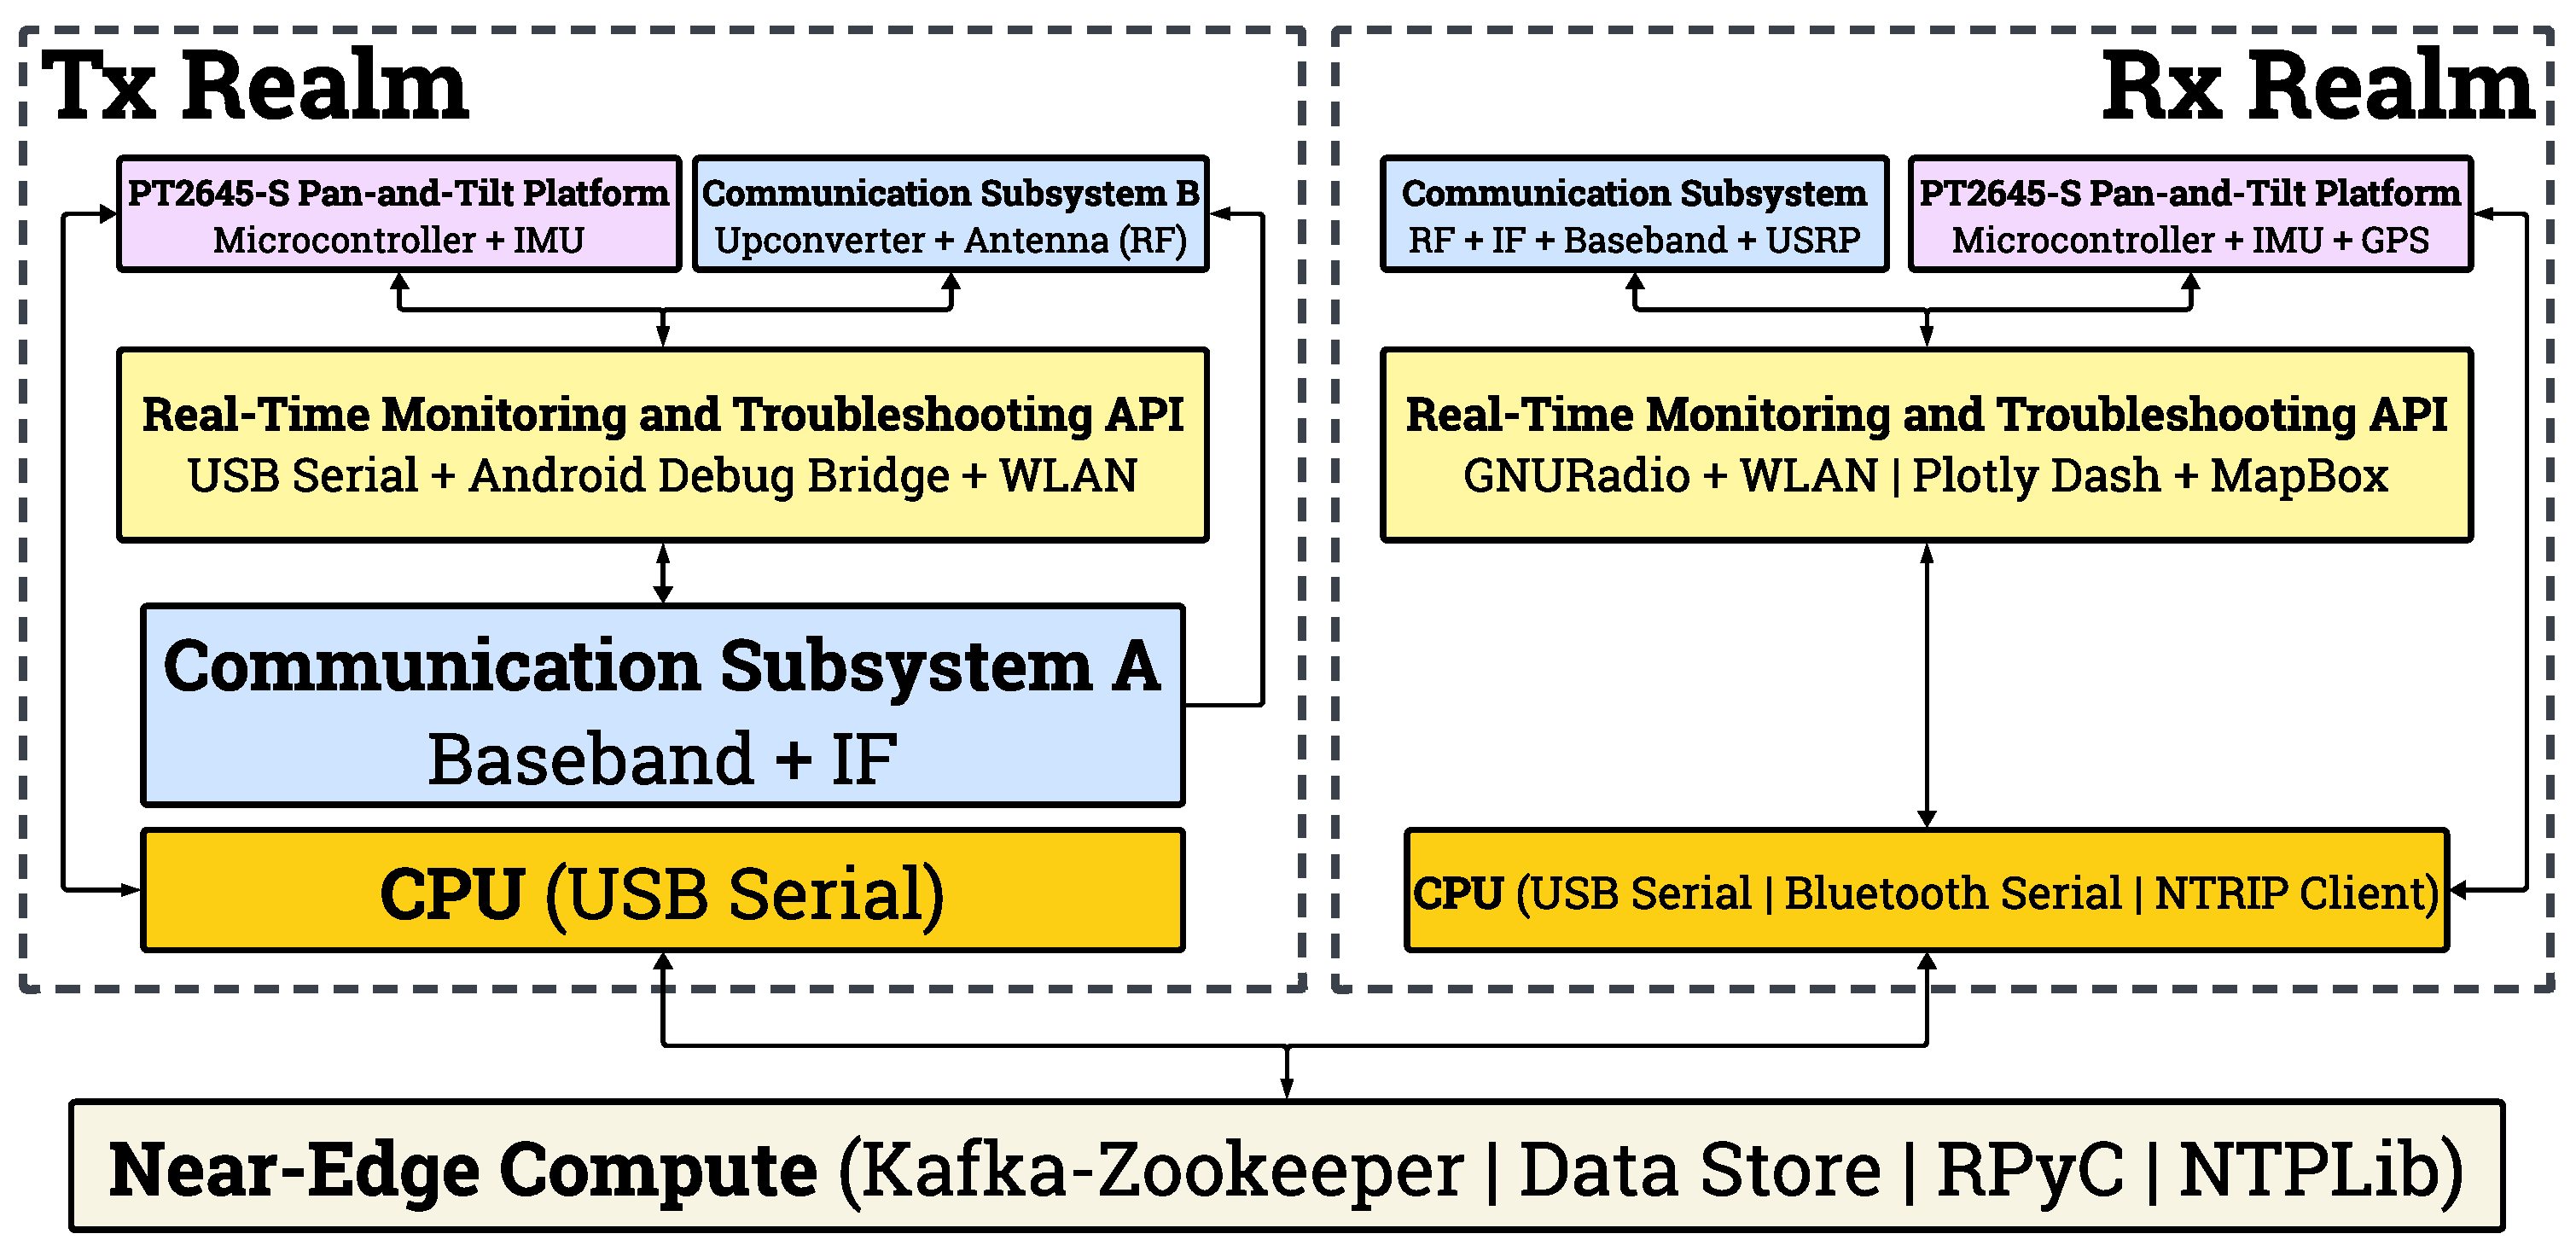
\includegraphics[width=0.94875\textwidth]{figs/system_architecture.pdf}
    \vspace{-2.5mm}
    \caption{The system architecture of our novel fully autonomous robotic beam-steering platform with a custom broadband sliding correlator channel sounder.}
    \vspace{-6mm}
    \label{F1}
\end{figure*}
\\\noindent{\textbf{Channel Sounder}}: The measurement system employed a custom broadband sliding correlator channel sounder at both the Tx and the Rx~\cite{Purdue}, each equipped with a Pseudorandom Noise (PN) sequence generator module producing the required known apriori signal for time-dilated cross-correlation studies, with the Rx module clocked at a slightly lower rate than the Tx; an up-/down-converter to transition between the \SI{2.5}{\giga\hertz} and \SI{28}{\giga\hertz} regimes; a vertically polarized WR-$28$ directional horn antenna; and other commercially available components. This setup is implemented according to the schematics shown in Fig.~\ref{F2a} and Fig.~\ref{F2b}. The operational specifications of the sounder are listed in Table~\ref{T3}, as detailed also in~\cite{Purdue}. As a part of the data logging operations at the Rx, complex-\SI{64}{} I/Q power delay profiles are recorded onboard an SSD storage by a GNURadio sink on a Raspberry Pi SBC via a USRP SDR.\\
\noindent{\textbf{Alignment and Tracking}}: To facilitate unrestricted rotational mobility for alignment and tracking in the horizontal and the vertical planes, at the Tx and the Rx, the WR-$28$ horn antenna is mounted on a PT$2645$-S open-loop pan-and-tilt platform, each driven by two HSR-$2645$CRH continuous rotation servos, with each servo actuating either yaw (horizontal) or pitch (vertical) alignment. These servos are controlled via PWM signals from an ATMega$328$P microcontroller with the angular position feedback provided by a BNO$080$ inertial motion unit. This principal axes positioning subsystem demonstrates an average accuracy of \SI{1.1}{\degree} across all coarse- and fine-grained yaw and pitch movements. Next, for seamless operations in V$2$X scenarios, this alignment platform is equipped with a geo-positioning subsystem constituting a UBlox ZED-F$9$P GPS module (with a GNSS multi-band antenna), with its positioning accuracy enhanced by RTCMv$3.0$ RTK correction streams over NTRIP. Demonstrating an average $3$D accuracy of \SI{17}{\centi\meter}, the relevant data members captured by this geo-positioning unit---namely, the coordinate (latitude, longitude, and ellipsoidal altitude), the horizontal speed and acceleration, and the heading, are communicated to the microcontroller as NMEA-$0183$ messages over an I$2$C serial peripheral bus. A glossary of the acronyms/protocols referenced above is given in Table~\ref{T1}. Since our measurement system revolves around a decoupled design with the alignment and tracking platform replicated at both the Tx and the Rx, a centralized nerve-center handles asynchronous module registration tasks via RPyC object proxying, global timing synchronization via NTP, and coordination between the Tx and Rx over a fault tolerant Apache Kafka messaging middleware. With an Apache Zookeeper broker manager serving as a distributed configuration, synchronization, and naming registry service for the Kafka cluster, the messages (events) generated by the principal axes positioning and geo-positioning subsystems are shared over Kafka message queues (known as topics, e.g., ``NSF\_POWDER\_RX\_GPS\_EVENTS''): the Tx subscribes to the alignment and geo-location messages published by the Rx, and vice-versa, resulting in a scalable event-driven modular architecture. Corroborated both onsite and in the laboratory, this publish-subscribe framework facilitates an average beam-steering response time of \SI{27.8}{\milli\second}, evaluated over ${\approx}$\SI{13000}{} interactions. With monitoring interactions exchanged over an Android debug bridge and system troubleshooting enabled via serial communication interfaces, our platform demonstrates remote orchestration capabilities - a critical necessity for mmWave propagation modeling in V$2$X settings. To augment these remote monitoring and troubleshooting features further, a GNURadio Qt GUI time-sink (with dynamic trigger levels) allows for real-time visualization of the recorded power delay profiles over an ad-hoc WLAN with the Raspberry Pi SBC; additionally, via the Plotly Dash and MapBox APIs, the Tx and Rx geo-locations are annotated with their relative alignment accuracies and visualized in real-time for onsite validation of routes traversed on the NSF POWDER experimental testbed.
\begin{figure*} [t]
    \centering
    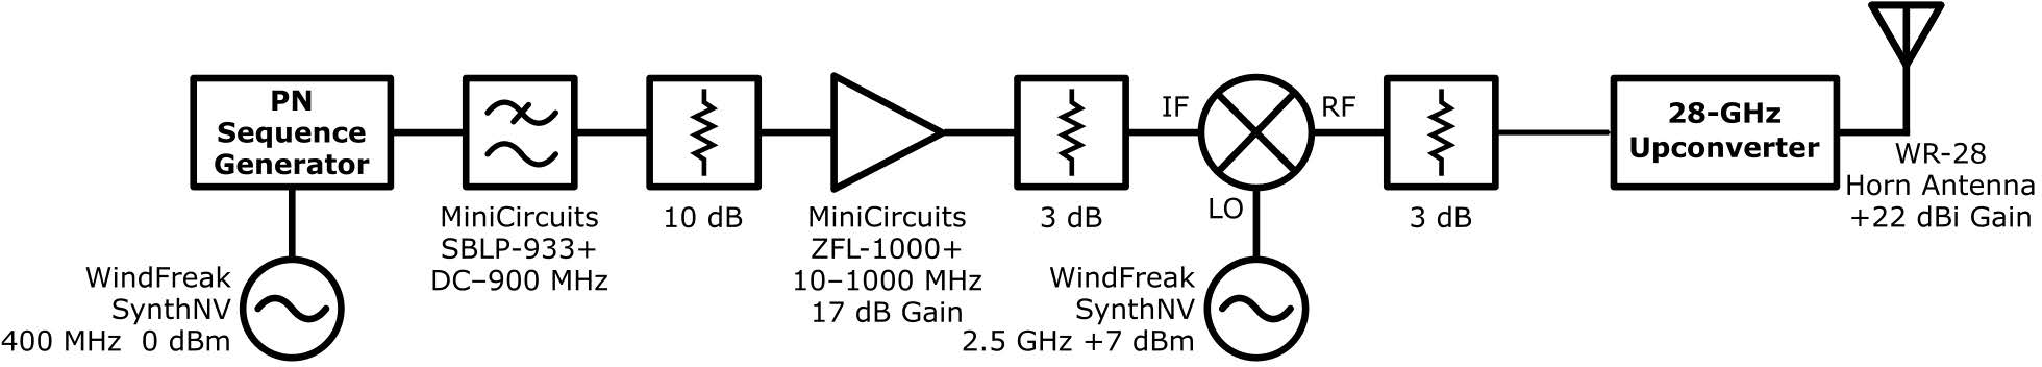
\includegraphics[width=0.95\linewidth]{figs/tx_schematic.pdf}
    \caption{The Tx circuit schematic with an up-converter, a WR-$28$ directional horn antenna, and other commercially available components.}
    \label{F2a}
\end{figure*}
\begin{figure*} [t]
    \centering
    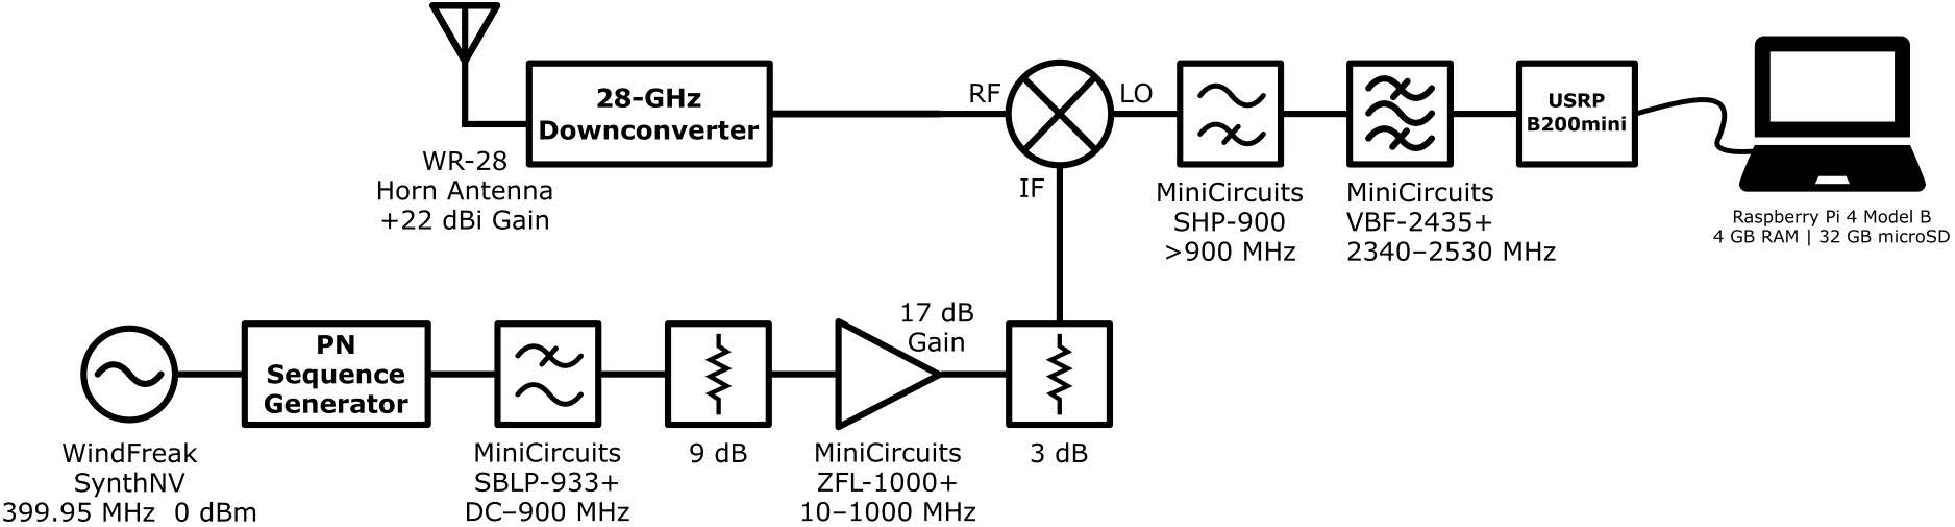
\includegraphics[width=0.95\linewidth]{figs/rx_schematic.pdf}
    \caption{The Rx circuit schematic with a down-converter, a WR-$28$ directional horn antenna, a USRP B$200$mini, and other commercially available components.}
    \label{F2b}
\end{figure*}
\renewcommand{\tabcolsep}{12pt}
\begin{table*} [tb]
	\centering
	\footnotesize
	\begin{tabular}{|l||l|}
		\hline
		Carrier Frequency & \SI{28}{\giga\hertz}\\
		\hline
		PN Chip Sequence Length & \SI{2047}{}\\
		\hline
		RF Bandwidth & \SI{800}{\mega\hertz}\\
		\hline
		Tx Chip Rate & \SI{400}{\mega{cps}}\\
		\hline
		Temporal Resolution & \SI{2.5}{\nano\second}\\
		\hline
		Rx Chip Rate & \SI{399.95}{\mega{cps}}\\
		\hline
		Tx Power & \SI{23}{\deci\bel{m}}\\
		\hline
		Tx/Rx Antenna Gain & \SI{22}{\deci\bel{i}}\\
		\hline
		Nominal Tx/Rx Antenna HPBW & \SI{15}{\degree}\\
		\hline
		Measured Tx/Rx Azimuth HPBW & \SI{10.1}{\degree}\\
		\hline
		Measured Tx/Rx Elevation HPBW & \SI{11.5}{\degree}\\
		\hline
		Maximum Measurable Pathloss & \SI{182}{\decibel}\\
		\hline
		GNURadio Sink Center Frequency & \SI{2.5}{\giga\hertz}\\
		\hline
		USRP Gain & \SI{76}{\decibel}\\
		\hline
		USRP Sampling Rate & \SI{2}{\mega{sps}}\\
		\hline
	\end{tabular}
	\vspace{-1mm}
	\caption{The specifications of the sliding correlator channel sounder used in our measurement campaign on the NSF POWDER experimental testbed~\cite{Purdue}.}
    \vspace{-6mm}
	\label{T3}
\end{table*}
\vspace{-8mm}

% Measurement campaign description and Data post-processing procedural explanation
\section{Measurements \& Post-Processing}\label{S3}
In this section, we discuss the operations involved in our \SI{28}{\giga\hertz} V$2$X measurement campaign on the NSF POWDER experimental testbed~\cite{POWDER}. First, we describe the calibration process; next, we outline the onsite deployment procedure; subsequently, we detail the post-processing steps involved in setting up the power delay profiles recorded at the Rx for pathloss evaluations including the empirical verifications of mmWave UMa ($3$GPP TR$38.901$ and ITU-R M$.2135$) and UMi (METIS and mmMAGIC) outdoor large-scale pathloss standards~\cite{MacCartneyModelsOverview}, multipath component extraction and associated parameter estimation via a custom implementation of the SAGE algorithm~\cite{SAGE}, spatial consistency analyses vis-\`{a}-vis Tx-Rx distance and alignment accuracy~\cite{SpatialConsistencyOriginal}, shadowing and accompanying fading studies under both static and dynamic blockages, multipath clustering investigations involving cluster inter-arrival times, cluster decay attributes, and RMS delay and direction spreads, along with the  empirical validations of favored mmWave statistical/parameterized channel models (SV~\cite{SV_Molisch}, QD~\cite{QDC_NIST}, and stochastic~\cite{Indoor60G}) in V$2$X applications.\\
\noindent{\textbf{Pre-deployment Calibration}}: After the Tx and Rx circuits for the sliding correlator channel sounder have been implemented as illustrated in Fig.~\ref{F2a} and Fig.~\ref{F2b}, a calibration procedure is carried out onsite to map the power calculated from the power delay profiles recorded by the USRP to reference measured power levels. The process of calibrating the measurement system before deployment ensures accurate received power calculations in the presence of imperfect circuit components, e.g., the Commscope LDF$4$-$50$A \SI{0.5}{{"}} coaxial cables employed at the Tx exhibit losses of up to \SI{0.12}{\deci\bel\per\meter} at \SI{2.5}{\giga\hertz}. Under \SI{0}{\deci\bel} and \SI{76}{\deci\bel} USRP gains, using a Keysight variable attenuator, the recorded power delay profiles are processed to determine the calculated powers mapped to corresponding reference power levels: the results of this procedure are employed in our numerical evaluations detailed in Sec.~\ref{S4} and Sec.~\ref{S5}~\cite{SPAVE_ICC}. We discuss the deployment of our measurement system onsite at the NSF POWDER experimental testbed next.\\
\noindent{\textbf{NSF POWDER Deployment}}: As described in Sec.~\ref{S2}, our measurement system assembly constitutes a fully autonomous beam-steering controller replicated at both the Tx and the Rx, their respective sounder circuits, and a centralized nerve center for aggregation (via RPyC), timing synchronization (via NTP), and coordination (via Kafka-Zookeeper). On the NSF POWDER testbed, this centralized nerve center is deployed on a high-availability cluster of four Dell R$740$ compute nodes at the Fort Douglas datacenter, with fault tolerance being a key feature to ensure storage redundancy for the recorded data. As depicted in Fig.~\ref{F3a}, the Tx is mounted on a building rooftop; while, as shown in Fig.~\ref{F3b}, the Rx is mounted on a van (or a push-cart) that is driven (or pushed) along unplanned routes onsite. Remote monitoring and troubleshooting is provided for validation of geo-positioning, alignment, and power delay profile samples. The goal of this measurement campaign was to obtain comprehensive datasets of site-specific measurements for evaluating the propagation behavior of \SI{28}{\giga\hertz} signals in V$2$X settings. Thus, our propagation modeling activities included V$2$I measurements under manual, partially, and fully autonomous alignment operations traversing $7$ routes spanning urban, suburban, and foliage radio environments. Although our platform is capable of double-directional measurements and facilitates easy scalability to MIMO settings, we focus only on beam-steered measurements in V$2$X scenarios for pathloss studies, spatial decoherence evaluations, shadowing and the associated fading studies under static and dynamic blockages, and investigations on the multipath clustering attributes.
\begin{figure*}[t]
    \centering
    \begin{subfigure}{0.355\linewidth}
        \centering
        \includegraphics[width=0.95\linewidth]{figs/tx_deployment.pdf}
        \caption{Tx Deployment at the William Browning Building}
        \label{F3a}
    \end{subfigure}
    \begin{subfigure}{0.635\linewidth}
        \centering
        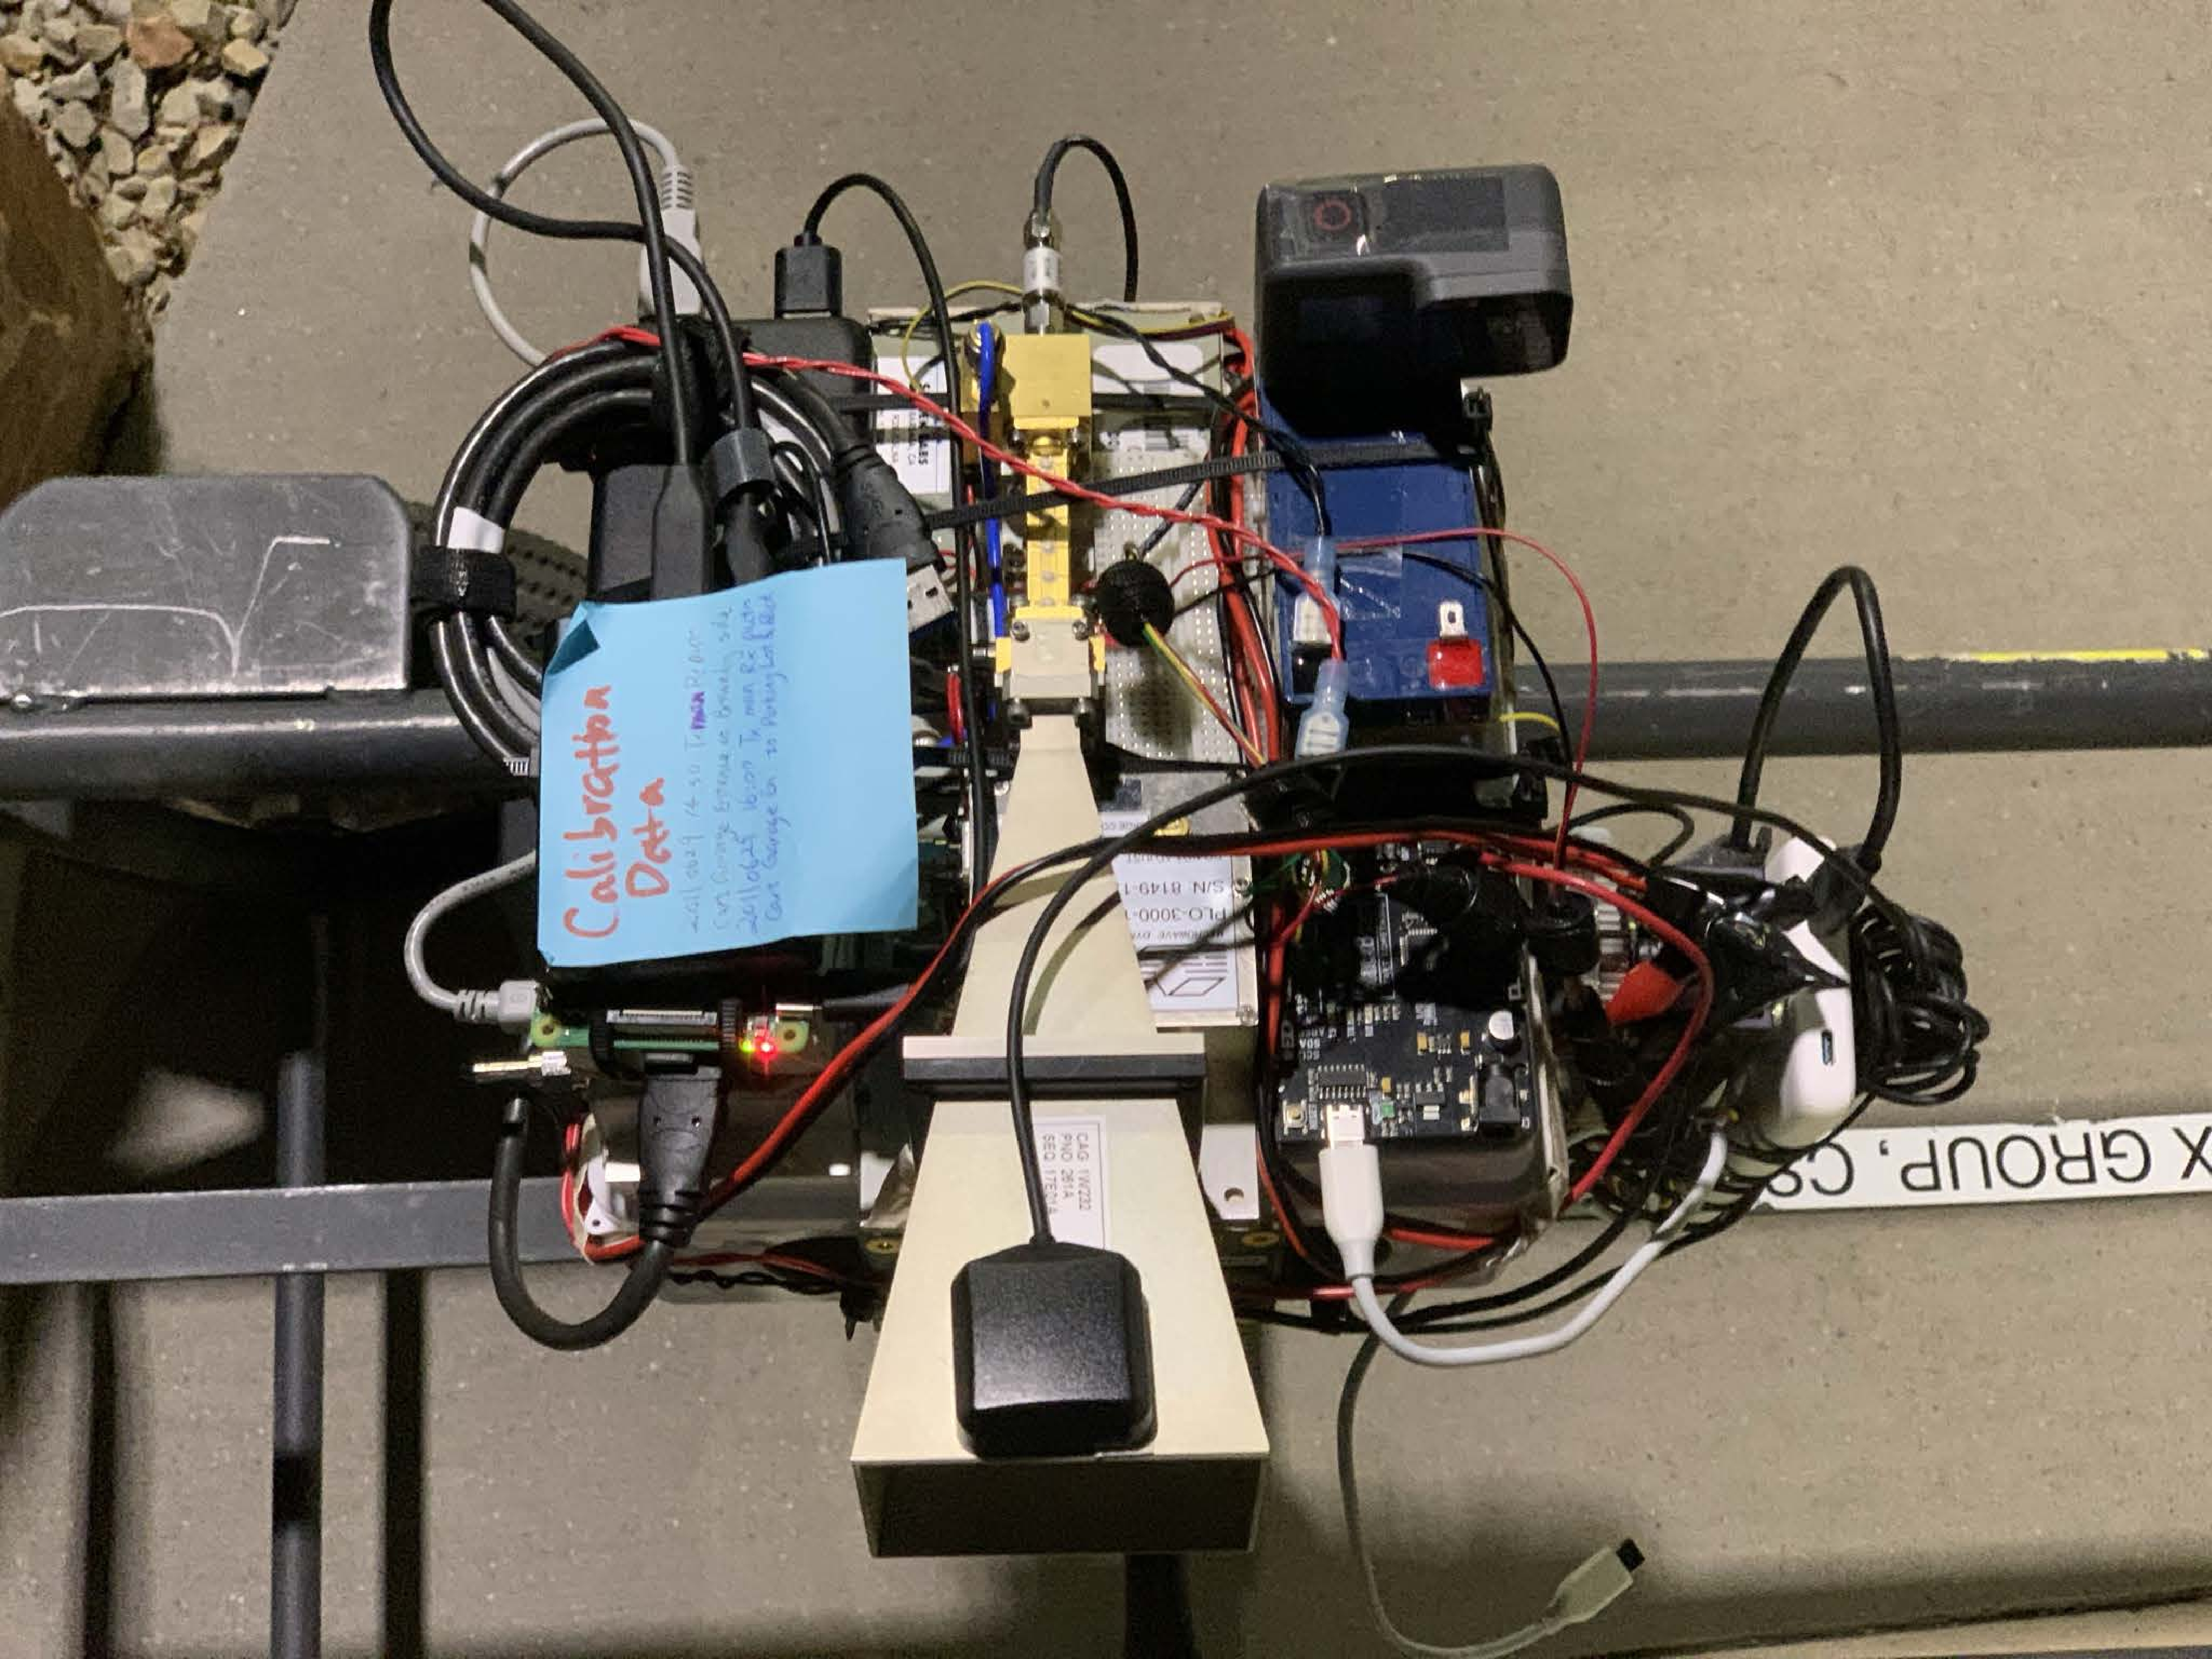
\includegraphics[width=0.95\linewidth]{figs/rx_deployment.pdf}
        \caption{Rx Push-Cart Deployment (Van mount involves the same setup. Datasets available on \href{http://ieee-dataport.org/12580}{DataPort}~\cite{DataPort}.)}
        \label{F3b}
    \end{subfigure}
    \vspace{-5mm}
    \caption{The Tx deployment atop the William Browning building at the NSF POWDER testbed site in Salt Lake City, UT, where the sounder circuits are housed in a climate-controlled enclosure with the antenna mounted on the pan-and-tilt platform (a); and the Rx deployment on a push-cart (or a minivan) (b).}
    \vspace{-5.45mm}
    \label{F3}
\end{figure*}
\\\noindent{\textbf{{Post-Processing}}: Using GNURadio utilities, the metadata file corresponding to the route-specific power delay profile records at the Rx is parsed to extract timestamp details, which are then associated with the geo-positioning and alignment logs at both the Tx and the Rx. The samples in each synchronized power delay profile segment are subjected to pre-filtering (via a low pass filter), time-windowing, and noise elimination (via a custom peak search and subsequent thresholding mechanism). Coupled with transmission power and antenna gain values, the received power levels obtained from these processed samples allow the visualization of pathloss maps on the Google Maps API (rendered via the Bokeh toolbox), and the evaluation of pathloss behavior as a function of Tx-Rx distance, along with validations against the $3$GPP TR$38.901$, ITU-R M$.2135$, METIS, and mmMAGIC standards~\cite{MacCartneyModelsOverview}. Additionally, shadow fading studies deliver key insights on signal propagation under static blockages (terrain, buildings); while pathloss vs time visualizations for routes dominant in dynamic blockages (pedestrians, moving/parked vehicles) allow examinations of the small-scale fading properties of mmWave signals (along with empirical validations against the D$2$D model~\cite{D2DHumanBlockage}). Next, the SAGE algorithm~\cite{SAGE}, employed for multipath component extraction, facilitates spatial consistency~\cite{SpatialConsistencyOriginal} and multipath clustering evaluations~\cite{Indoor60G}. In particular, under variations in distance and alignment accuracy, we probe signal decoherence patterns via the spatial autocorrelation coefficient~\cite{MacCartneySpatialStatistics}; also, we analyze the multipath clustering characteristics of \SI{28}{\giga\hertz} signals in V$2$X settings vis-\`{a}-vis cluster inter-arrival times, cluster decay attributes, and RMS delay and direction spreads; lastly, these studies allow the empirical validations of mmWave channel models, viz., SV~\cite{SV_Molisch}, QD~\cite{QDC_NIST}, and stochastic~\cite{Indoor60G}).
\vspace{-6mm}

% Numerical evaluations I: Pathloss studies and Spatial consistency evaluations
\section{Pathloss and Spatial Consistency Evaluations}\label{S4}
In this section, we outline the initial sets of results derived from our evaluations on the collected datasets. We first briefly study the radiation patterns of the directional horn antennas and the results of our calibration procedure, both of which are then employed in our ensuing evaluations; next, we analyze the empirical pathloss results attained from our measurements along a diverse set of routes and validate them against popular outdoor pathloss standards~\cite{MacCartneyModelsOverview}; subsequently, we detail our spatial consistency evaluations and examine the decoherence behavior of mmWave signals under variations in distance and alignment accuracy~\cite{SpatialConsistencyOriginal}; additionally, we outline the insights obtained from our shadow fading studies under the effects of static geometry induced losses; and finally, we describe our findings on the small-scale fading attributes of the obstructed \SI{28}{\giga\hertz} signals under dynamic blockages in V$2$X scenarios, in addition to their comparisons with the D$2$D model~\cite{D2DHumanBlockage}.\\
\noindent{\textbf{Antenna Patterns and Calibration}}: Obtained via empirical recordings of the WR-$28$ antenna's operational characteristics, Fig.~\ref{F4} illustrates its normalized measured $2$D radiation patterns along the azimuth and elevation directions: these enable us to compute the gains at specific locations along a route and at specific degrees of alignment, crucial for our ensuing analyses. As evident from this illustration, the WR-$28$ horn antennas employed in our propagation modeling campaign are highly directional, thus necessitating the need for an accurate and reliable beam-steering system, particularly in V$2$X settings. Furthermore, conducting the pre-deployment calibration procedure as outlined in Sec.~\ref{S3}, we derive a linear relationship between the measured received power levels and their calculated power values corresponding to artificial attenuation injections into the signal path between the Tx and the Rx. This calibration relationship (for both \SI{0}{\deci\bel} and \SI{76}{\deci\bel} USRP gain values) allows us to account for losses introduced into our measurements due to imperfect circuit components: refer to our preliminary work in~\cite{SPAVE_ICC} for additional details.
\begin{figure*} [t]
    \centering
    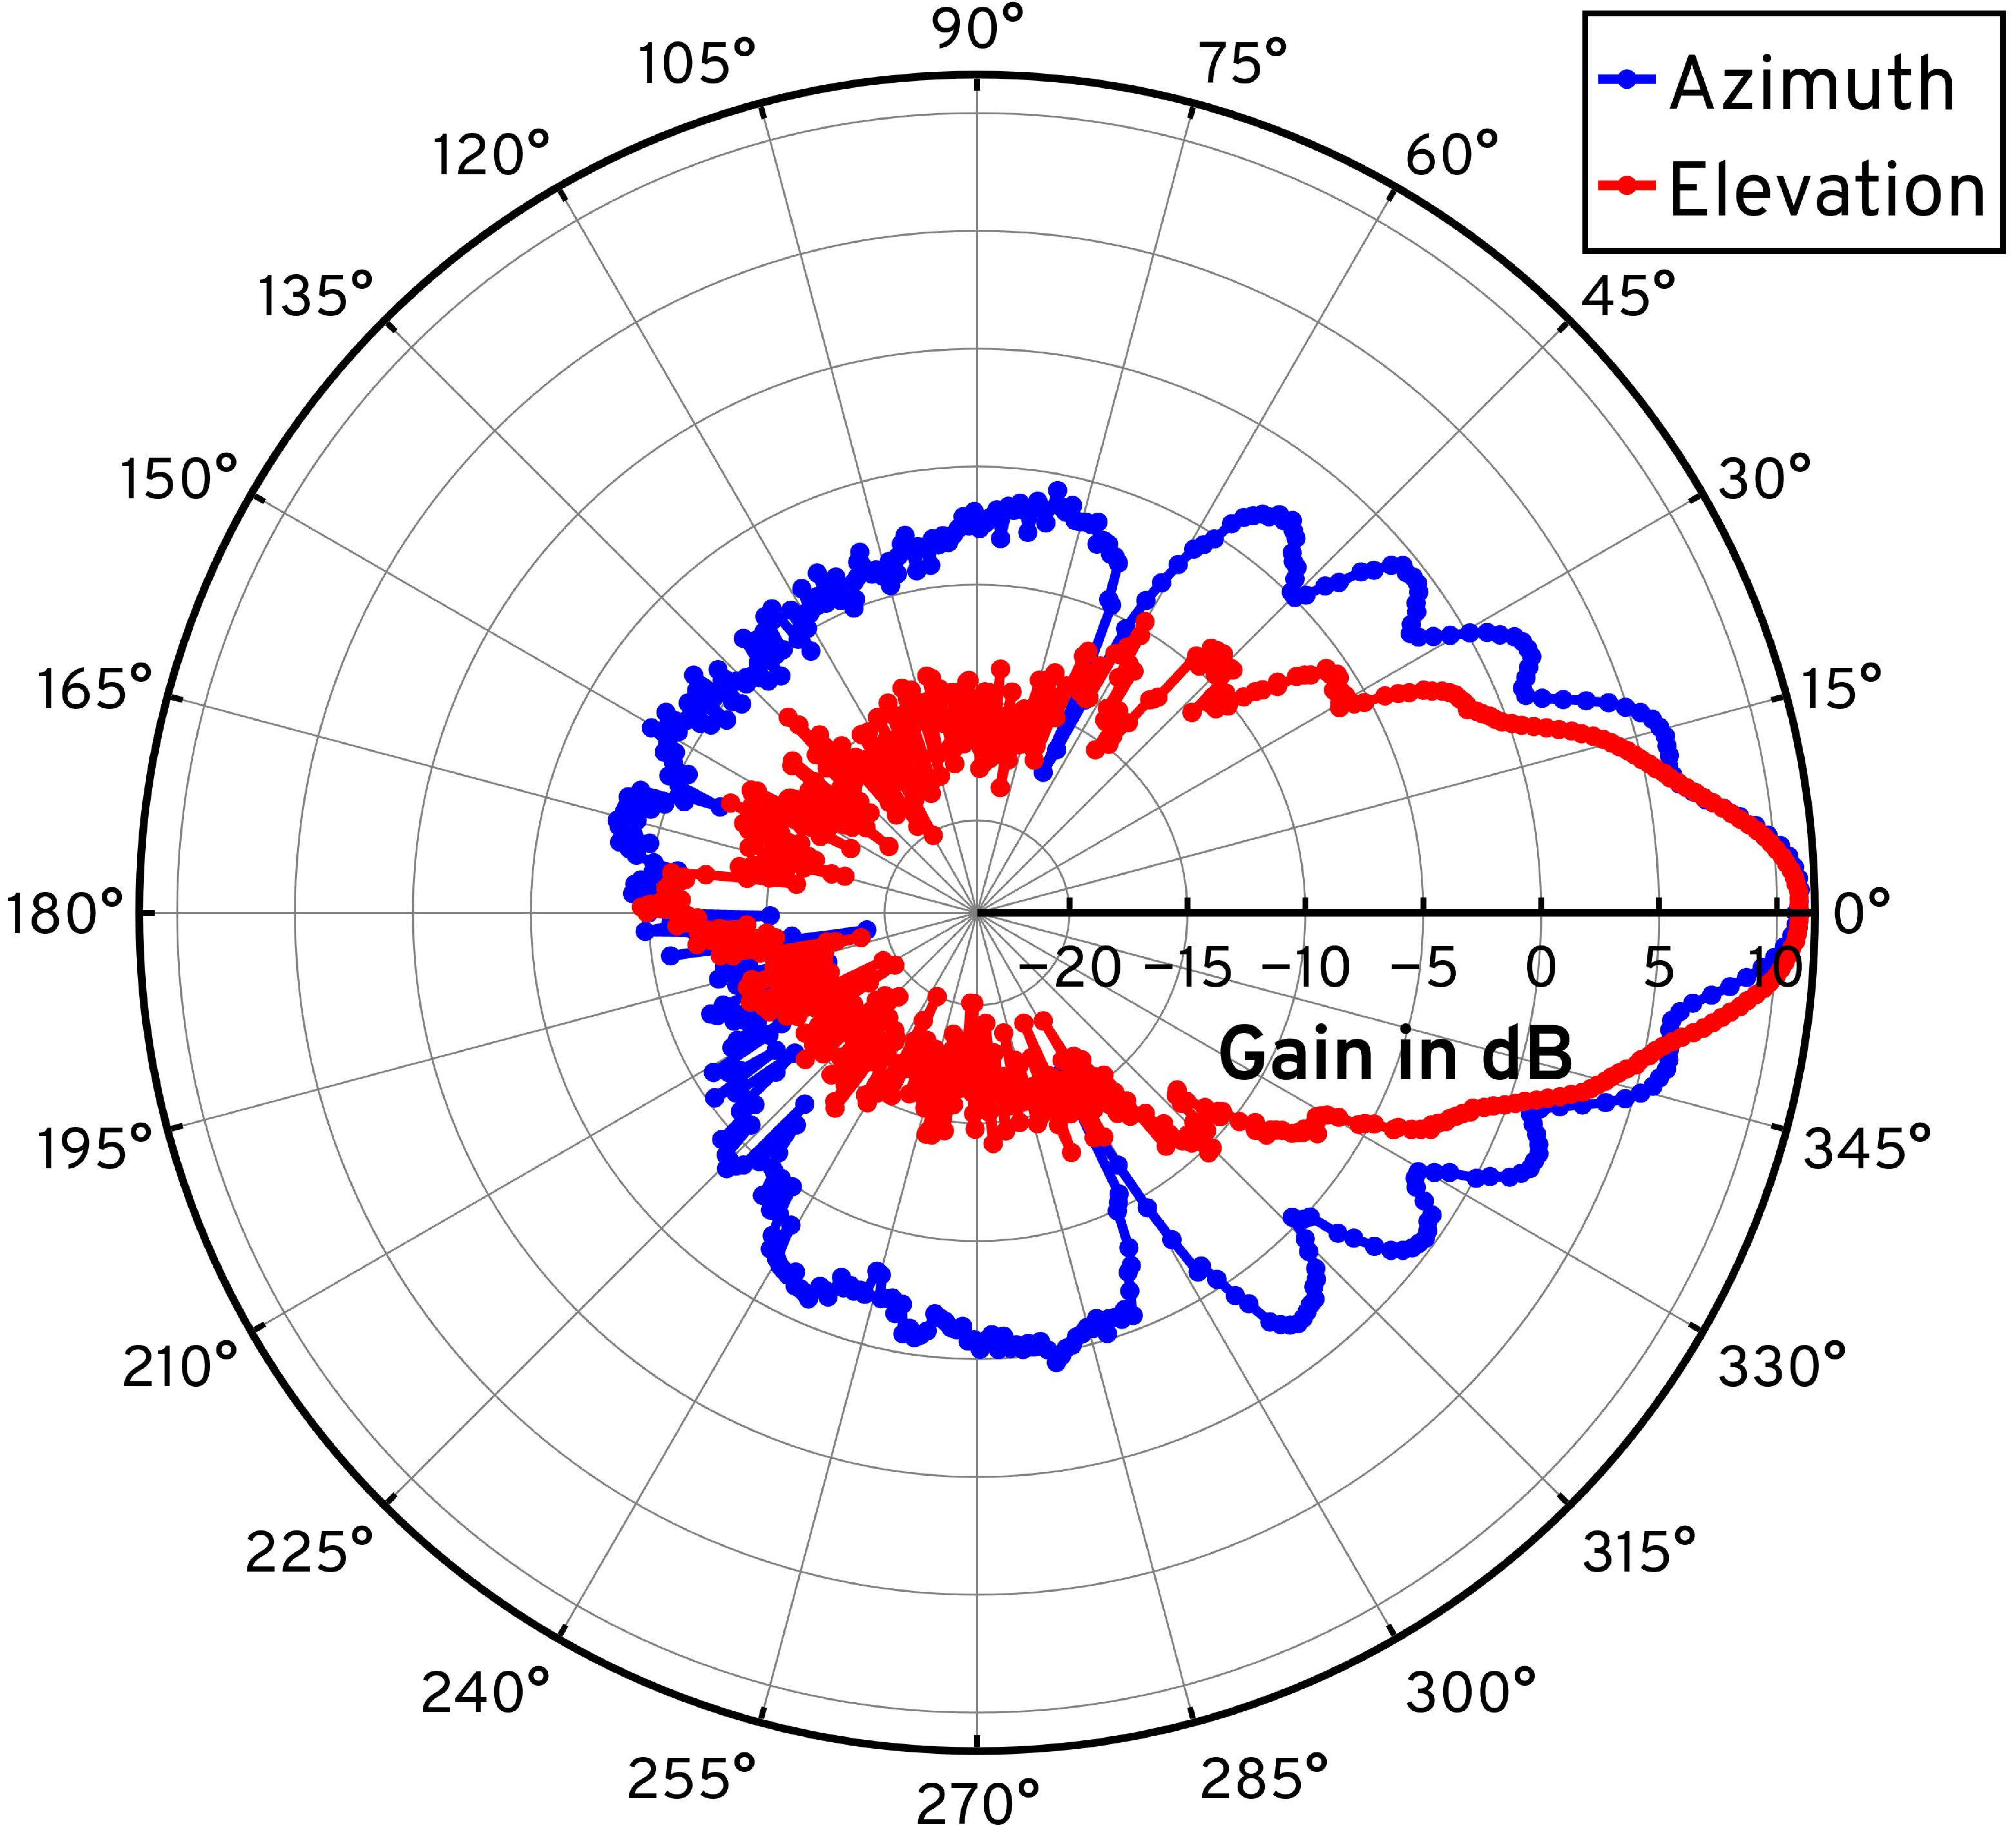
\includegraphics[width=0.55\linewidth]{figs/antenna_patterns.pdf}
    \caption{The normalized measured $2$D radiation patterns along the azimuth and elevation directions for the WR-$28$ horn antennas (\href{https://codeocean.com/capsule/9545863/tree}{CodeOcean}~\cite{CodeOcean}; \href{http://ieee-dataport.org/12580}{DataPort}~\cite{DataPort}).}
    \vspace{-6mm}
    \label{F4}
\end{figure*}
\\\noindent{\textbf{Pathloss Studies}}: Upon post-processing the collected datasets (geo-positioning logs, alignment samples, and power delay profiles) according to the processing operations detailed in Sec.~\ref{S3}, we compute the signal power at the Rx (with calibration offsets); subsequently, knowing the Tx power and the antenna gains, we compute the pathloss experienced at each Rx position around a specific route onsite. Fig.~\ref{F5a} and Fig.~\ref{F5b} depict the pathloss heat-maps (superimposed on Google hybrid maps) for the urban campus routes traversed during our campaign---namely, the route around President's Circle and the route around $100$ S St, respectively. With the Tx affixed atop the William Browning building, for the urban campus route around President's Circle (Fig.~\ref{F5a}), the Rx was mounted on a minivan and driven around onsite, while for the urban campus route around $100$ S St (Fig.~\ref{F5b}), the Rx was mounted on a cart and pushed around onsite. It is evident from these pathloss heat-maps in Fig~\ref{F5a} and Fig.~\ref{F5b} that the received signals along the $100$ S St route (Fig.~\ref{F5b}) as opposed to those along the President's Circle route (Fig.~\ref{F5a}) experience relatively lower pathloss due to their comparatively smaller Tx-Rx distances and smaller Tx-Rx relative velocities (cart vs van). Also, note that in Fig.~\ref{F5b}, since at certain locations, the Rx is hidden behind tall buildings, the obstacle induced losses (i.e., shadow fading) have a dominant impact on the received signal strength: this is discussed in further detail later in this section. In a similar vein, Fig.~\ref{F6a} and Fig.~\ref{F6b} depict the pathloss heat-maps (superimposed on Google hybrid maps) of the foliage dominated route (campus vegetation around the Olpin Union building) and the suburban neighborhood route (around S Wolcott St), respectively. With the Tx affixed atop the William Browning building, for both these routes, the Rx is mounted on a cart and pushed around onsite. Evaluating the differences in received signal power trends between these two routes, we observe that, across similar Tx-Rx distances, the foliage dominated environment (Fig.~\ref{F6a})---as opposed to the suburban environment which presents a considerably lower vegetation density (Fig.~\ref{F6b})---demonstrates larger pathloss due to foliage induced diffractions introduced into the signal path.\\
\begin{figure*} [t]
    \centering
    \begin{subfigure}{0.564\linewidth}
        \centering
        \includegraphics[width=0.95\linewidth]{figs/urban_campus_pathloss_1.pdf}
        \caption{Urban Campus: President's Circle (\href{https://codeocean.com/capsule/9545863/tree}{CodeOcean}~\cite{CodeOcean}; \href{http://ieee-dataport.org/12580}{DataPort}~\cite{DataPort})}
        \label{F5a}
    \end{subfigure}
    \begin{subfigure}{0.426\linewidth}
        \centering
        \includegraphics[width=0.95\linewidth]{figs/urban_campus_pathloss_2.pdf}
        \caption{Urban Campus: $100$ S St (\href{https://codeocean.com/capsule/9545863/tree}{CodeOcean}~\cite{CodeOcean}; \href{http://ieee-dataport.org/12580}{DataPort}~\cite{DataPort})}
        \label{F5b}
    \end{subfigure}
    \vspace{-5mm}
    \caption{The pathloss values superimposed on a Google hybrid map for the urban campus routes: President's Circle (Rx on a minivan) and $100$ S St (Rx on a push-cart). The color palette dots denote the Rx positions along the route and the blue diamond denotes the Tx location atop the William Browning building.}
    \vspace{-3mm}
    \label{F5}
\end{figure*}
\indent{Ensuing} these heat-map plots of the pathloss experienced by \SI{28}{\giga\hertz} signals around various vehicular routes traversed onsite, we compare the pathloss vs distance behavior of mmWave signals in our measurement campaign with popular outdoor micro- and macro-cellular pathloss standards ($3$GPP TR$38.901$, ITU-R M$.2135$, METIS, and mmMAGIC~\cite{MacCartneyModelsOverview}). These popular standards constitute both line-of-sight as well as non-line-of-sight models, with a Tx height of $h_{\text{Tx}}{\approx}$\SI{25}{\meter} and a Tx-Rx $2$D separation range of \SI{10}{\meter}${\leq}d_{2\text{D}}{\leq}$\SI{5000}{\meter}, which match the deployment specifications of our campaign, making them suitable candidates for empirical validations. In particular, as shown in Fig.~\ref{F7a}, evaluating the pathlosses computed from our collected measurements against these standards for the urban campus (President's Circle and $100$ S St), suburban neighborhood (S Wolcott St), and foliage environment (Olpin Union) routes, we observe that all these pathloss standards fail to accurately capture the pathloss vs log-distance behavior of \SI{28}{\giga\hertz} signals in V$2$X propagation scenarios. Specifically, we notice that, employing a linear curve-fitting procedure (via a floating intercept model) to extrapolate the pathloss values across an extended range of Tx-Rx distances (solid lines for our measurements and dashed lines for the subsequent extrapolation), there is a significant discrepancy between our measurements and the standards, in the characteristics of the pathloss across such distances. Therefore, we can conclude that the $3$GPP TR$38.901$, ITU-R M$.2135$, METIS, and mmMAGIC large-scale outdoor pathloss standards require considerable improvements to account for the nuances in mmWave propagation in V$2$X applications.
\begin{figure*} [t]
    \centering
    \begin{subfigure}{0.5565\linewidth}
        \centering
        \includegraphics[width=0.95\linewidth]{figs/foliage_pathloss.pdf}
        \caption{Foliage Environment: Olpin Union (\href{https://codeocean.com/capsule/9545863/tree}{CodeOcean}~\cite{CodeOcean}; \href{http://ieee-dataport.org/12580}{DataPort}~\cite{DataPort})}
        \label{F6a}
    \end{subfigure}
    \begin{subfigure}{0.4335\linewidth}
        \centering
        \includegraphics[width=0.95\linewidth]{figs/suburban_pathloss.pdf}
        \caption{Suburban Neighborhood: S Wolcott St (\href{https://codeocean.com/capsule/9545863/tree}{CodeOcean}~\cite{CodeOcean}; \href{http://ieee-dataport.org/12580}{DataPort}~\cite{DataPort})}
        \label{F6b}
    \end{subfigure}
    \vspace{-5mm}
    \caption{The pathlosses superimposed on a Google hybrid map for foliage environment (Rx on a push-cart) and suburban neighborhood (Rx on a push-cart) routes. Here, the color palette dots denote the Rx positions along the route and the blue diamond denotes the Tx location atop the William Browning building.}
    \vspace{-3mm}
    \label{F6}
\end{figure*}
\\\noindent{\textbf{SAGE Algorithm}}: To analyze the multipath propagation characteristics of \SI{28}{\giga\hertz} signals during our measurement campaign, we employ a custom implementation of the SAGE algorithm~\cite{SAGE} to extract the complex attenuations ($\alpha$), the delays ($\tau$), the Doppler shifts ($\nu$), and the AoA values ($\phi,\theta$) of the multiple specular paths arriving at the Rx while traversing a particular route onsite. Directly solving for the exact high-resolution maximum likelihood estimate of this parameter vector ($\boldsymbol{\xi}_{l}{=}[\alpha_{l},\tau_{l},\nu_{l},\phi_{l},\theta_{l}]^{\intercal},l{=}1,2,{\dots}$) involves prohibitively large computation times~\cite{SAGE}. Thus, the SAGE algorithm solves for an approximate estimate of $\boldsymbol{\xi}_{l}$ via iterative executions of the E-step which computes the expectation of the log-likelihood given the observations and the previous estimate, and the M-step which computes the current estimate by maximizing over the E-step result. This iterative execution occurs until convergence, i.e., the change in parameter values across consecutive iterations is lower than a preset threshold.
\begin{figure*} [t]
    \centering
    \begin{subfigure}{0.49\linewidth}
        \centering
        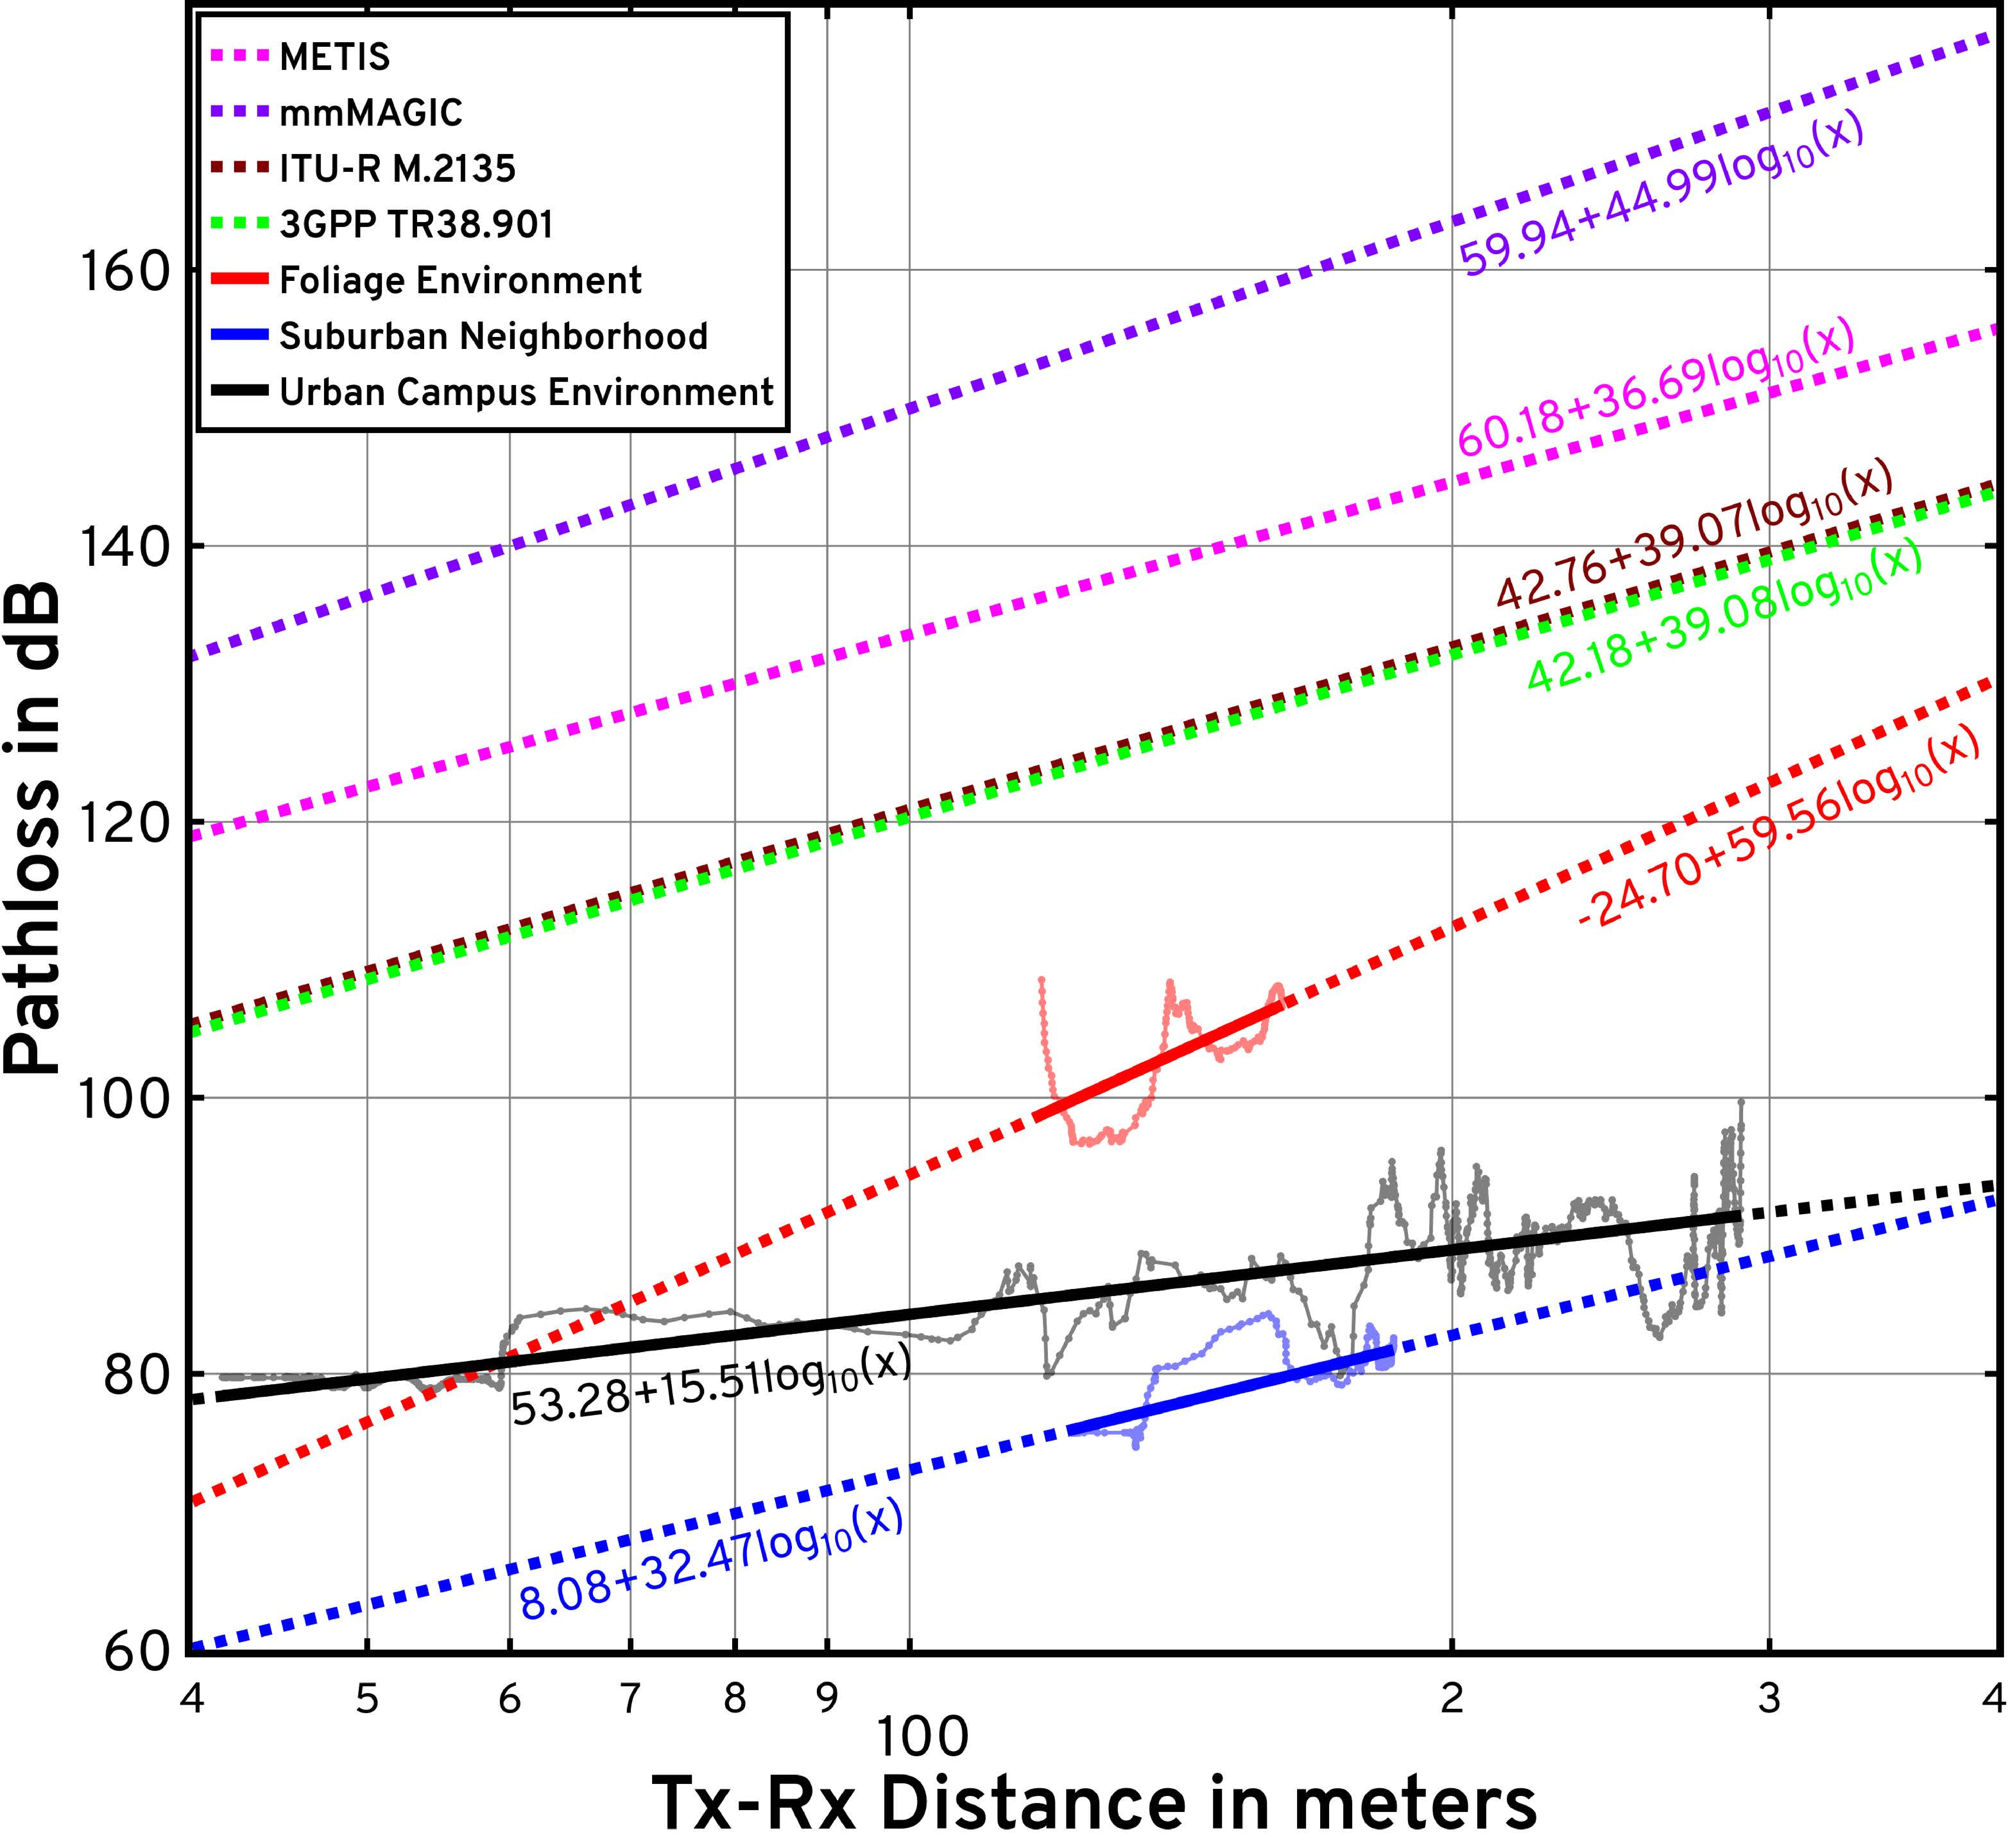
\includegraphics[width=0.95\linewidth]{figs/pathloss_vs_distance.pdf}
        \caption{Pathloss vs Tx-Rx Distance (\href{https://codeocean.com/capsule/9545863/tree}{CodeOcean}~\cite{CodeOcean}; \href{http://ieee-dataport.org/12580}{DataPort}~\cite{DataPort})}
        \label{F7a}
    \end{subfigure}
    \begin{subfigure}{0.5\linewidth}
        \centering
        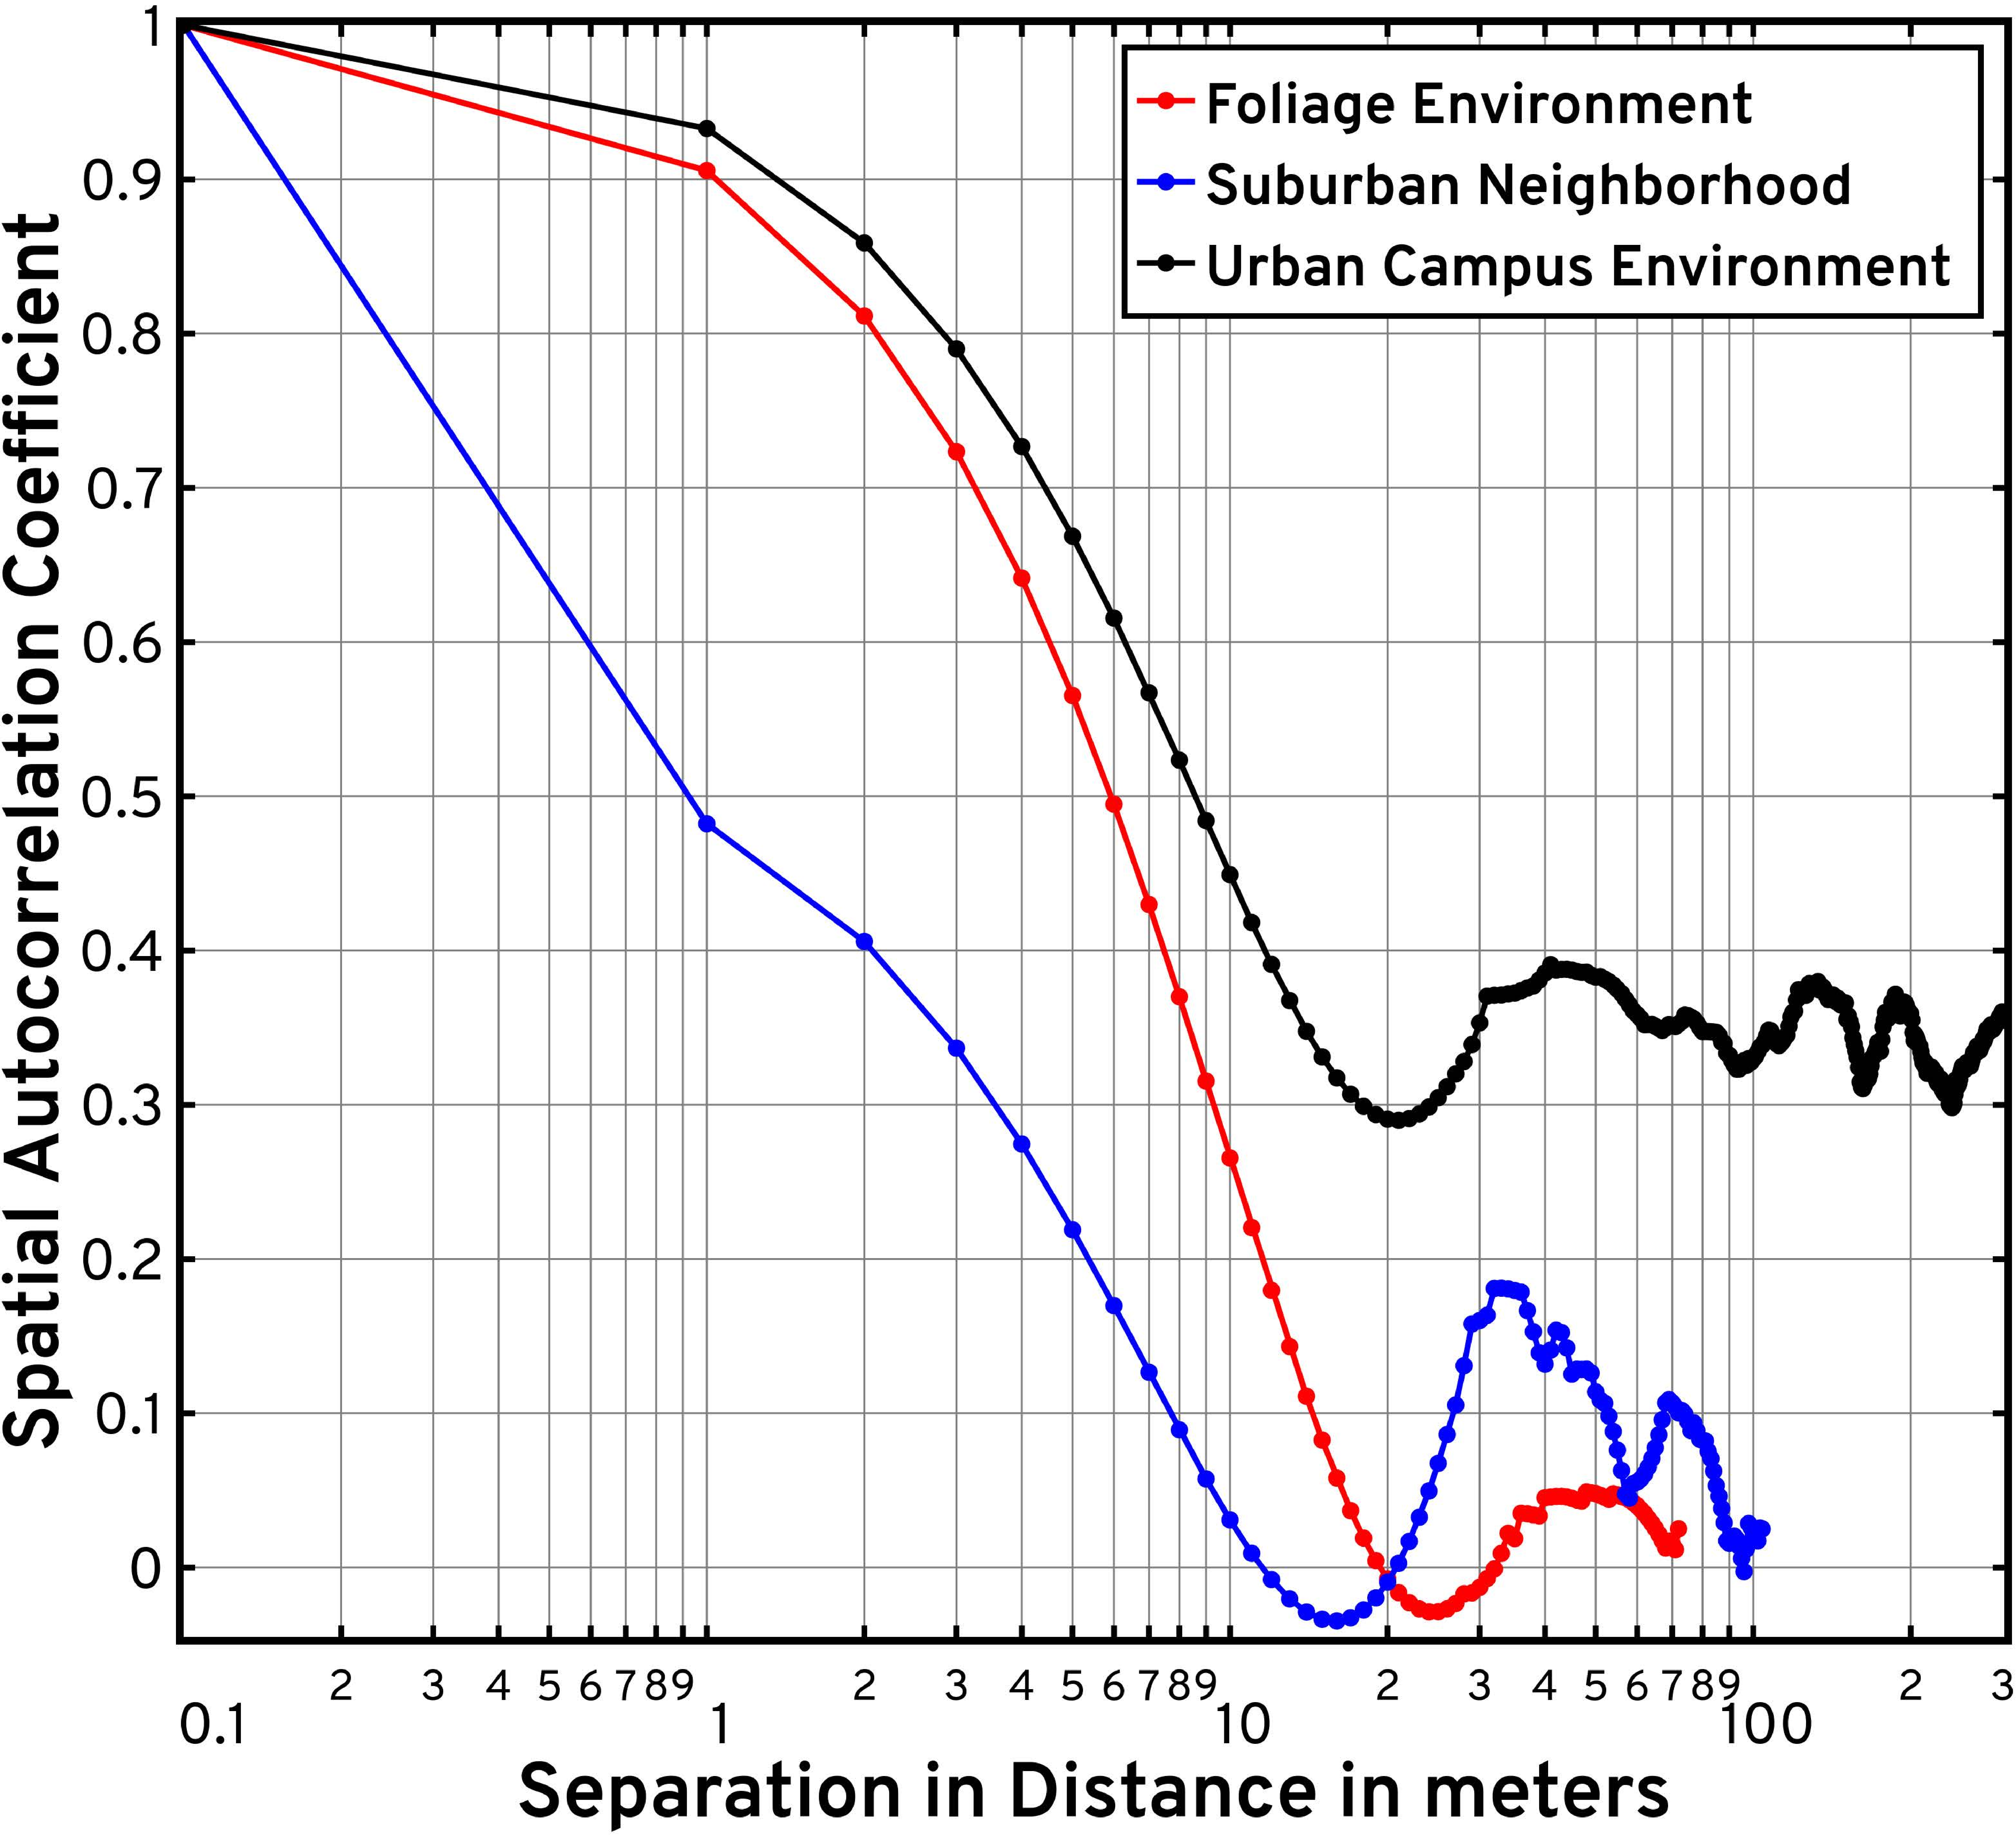
\includegraphics[width=0.95\linewidth]{figs/spatial_consistency_vs_distance.pdf}
        \caption{Spatial Consistency vs Distance Separation (\href{https://codeocean.com/capsule/9545863/tree}{CodeOcean}~\cite{CodeOcean}; \href{http://ieee-dataport.org/12580}{DataPort}~\cite{DataPort})}
        \label{F7b}
    \end{subfigure}
    \vspace{-5mm}
    \caption{A plot of the measured and extrapolated pathloss (in dB) vs log-distance (in meters) for \SI{28}{\giga\hertz} signals in V$2$X settings, and their comparisons against the $3$GPP TR$38.901$, ITU-R M.$2135$, METIS, and mmMAGIC standards---with the solid lines denoting our measurements and the dashed lines denoting the corresponding fitted models (a); and a plot of the spatial autocorrelation coefficient vs distance separation (b), i.e., $\rho(\Delta d)$ vs log-distance (in meters).}
    \vspace{-5mm}
    \label{F7}
\end{figure*}
\\\noindent{\textbf{Spatial Consistency}}: In this subsection, to study the spatial decoherence behavior of \SI{28}{\giga\hertz} signals in V$2$X scenarios, we evaluate the spatial autocorrelation coefficient along specific Rx routes under the effects of separations in distance and alignment accuracy. Herein, we first describe the mathematical modeling underlying the computation of this autocorrelation coefficient, after which we outline the insights gained from our results on the decoherence characteristics of \SI{28}{\giga\hertz} signals in V$2$X settings under distance and alignment accuracy effects. The small-scale spatial autocorrelation coefficient is a metric to characterize the coherence between the voltage amplitudes of received signals across variations in distances and alignment accuracies. With $\mathcal{I} \triangleq \{1,2,{\dots},I\}$ as the index set, we define a route in our measurement campaign as a set of $4$-tuples, i.e., $\mathcal{R} \triangleq \{\mathcal{T}_{i} \triangleq \left(\mathbf{x}_{i}, \mathbf{y}_{i}, \phi_{i}, \mathcal{M}_{i}\right) \suchthat i \in \mathcal{I}\}$, where $\mathbf{x}_{i}$ denotes the $3$D position vector of the Rx, $\mathbf{y}_{i}$ denotes the $3$D position vector of the Tx, and $\phi_{i}$ denotes the accuracy of alignment between the Tx and Rx horn antennas (i.e., deviation from perfect alignment). Let $\mathcal{J}_{i} \triangleq \{1,2,{\dots},J_{i}\}$ represent the index set for the collection of measurements obtained at the route configuration index $i \in \mathcal{I}$; therefore, the corresponding set of measurements is defined as $\mathcal{M}_{i} \triangleq \{\mathbf{m}_{i,j} \suchthat j \in \mathcal{J}_{i}\}$. As detailed in Sec.~\ref{S3}, each vector of received samples $\mathbf{m}_{i,j}$ undergoes processing via pre-filtering, time-windowing, and noise elimination; next, with propagation delay bins $\boldsymbol{\tau} \triangleq \{\tau_{1},\tau_{2},{\dots},\tau_{L}\}$ (e.g., $1$ ns to $1000$ ns quantization), we extract the amplitudes of the Multi-Path Components (MPCs) at these delay bins using the SAGE algorithm~\cite{SAGE}, i.e., $\forall i \in \mathcal{I}$, we define the local set of MPC amplitudes across all delay bins as $\tilde{\mathcal{M}}_{i} \triangleq \left\{\Big[A_{i,j}(\tau_{1}), A_{i,j}(\tau_{2}), \dots, A_{i,j}(\tau_{L})\Big]^{\mathsf{T}} \suchthat j \in \mathcal{J}_{i}\right\}$.
\vspace{1mm}
With the Tx fixed ($\mathbf{y}_{i} = \mathbf{y}, \forall i \in \mathcal{I}$), we define the following two sets as evaluation conditions to compute the spatial autocorrelation coefficient~\cite{MacCartneySpatialStatistics} under changes in their respective separation variables, i.e., separation in distance $\Delta d$ and in alignment $\Delta \phi$:
\begin{align}\label{E}
    \mathcal{I}(\Delta d)&{\triangleq}\left\{(i,i'){\in}\binom{\mathcal{I}}{2}:\norm{\mathbf{x}_{i}{-}\mathbf{x}_{i'}}{=}\Delta d,\phi_{i}{=}\phi_{i'}\right\};\\
    \mathcal{I}(\Delta\phi)&{\triangleq}\left\{(i,i'){\in}\binom{\mathcal{I}}{2}:\mathbf{x}_{i}{=}\mathbf{x}_{i'},\abs{\phi_{i}{-}\phi_{i'}}{=}\Delta\phi\right\}\label{Ea};
\end{align}
where $\mathcal{I}(\Delta d)$ and $\mathcal{I}(\Delta \phi)$ denote the sets employed to compute the spatial autocorrelation coefficient for changes in distance and alignment accuracy, respectively. Here, to ensure that our resultant spatial consistency analyses capture the effects of distance only, the constituent route index pairs in $\mathcal{I}(\Delta d)$ should be separated by a distance of $\Delta d$ ($\norm{\mathbf{x}_{i}{-}\mathbf{x}_{i'}}{=}\Delta d$) while having the same alignment accuracy ($\phi_{i}{=}\phi_{i'}$). Similarly, the definition of $\mathcal{I}(\Delta \phi)$ ensures that our analyses accurately captures the effects of alignment accuracy only, by enforcing equal distance ($\mathbf{x}_{i}{=}\mathbf{x}_{i'}$) and $\Delta \phi$ separation in alignment accuracy ($\abs{\phi_{i}{-}\phi_{i'}}{=}\Delta \phi$) for the constituent route index pairs.\\
\begin{figure*} [t]
    \centering
    \begin{subfigure}{0.4925\linewidth}
        \centering
        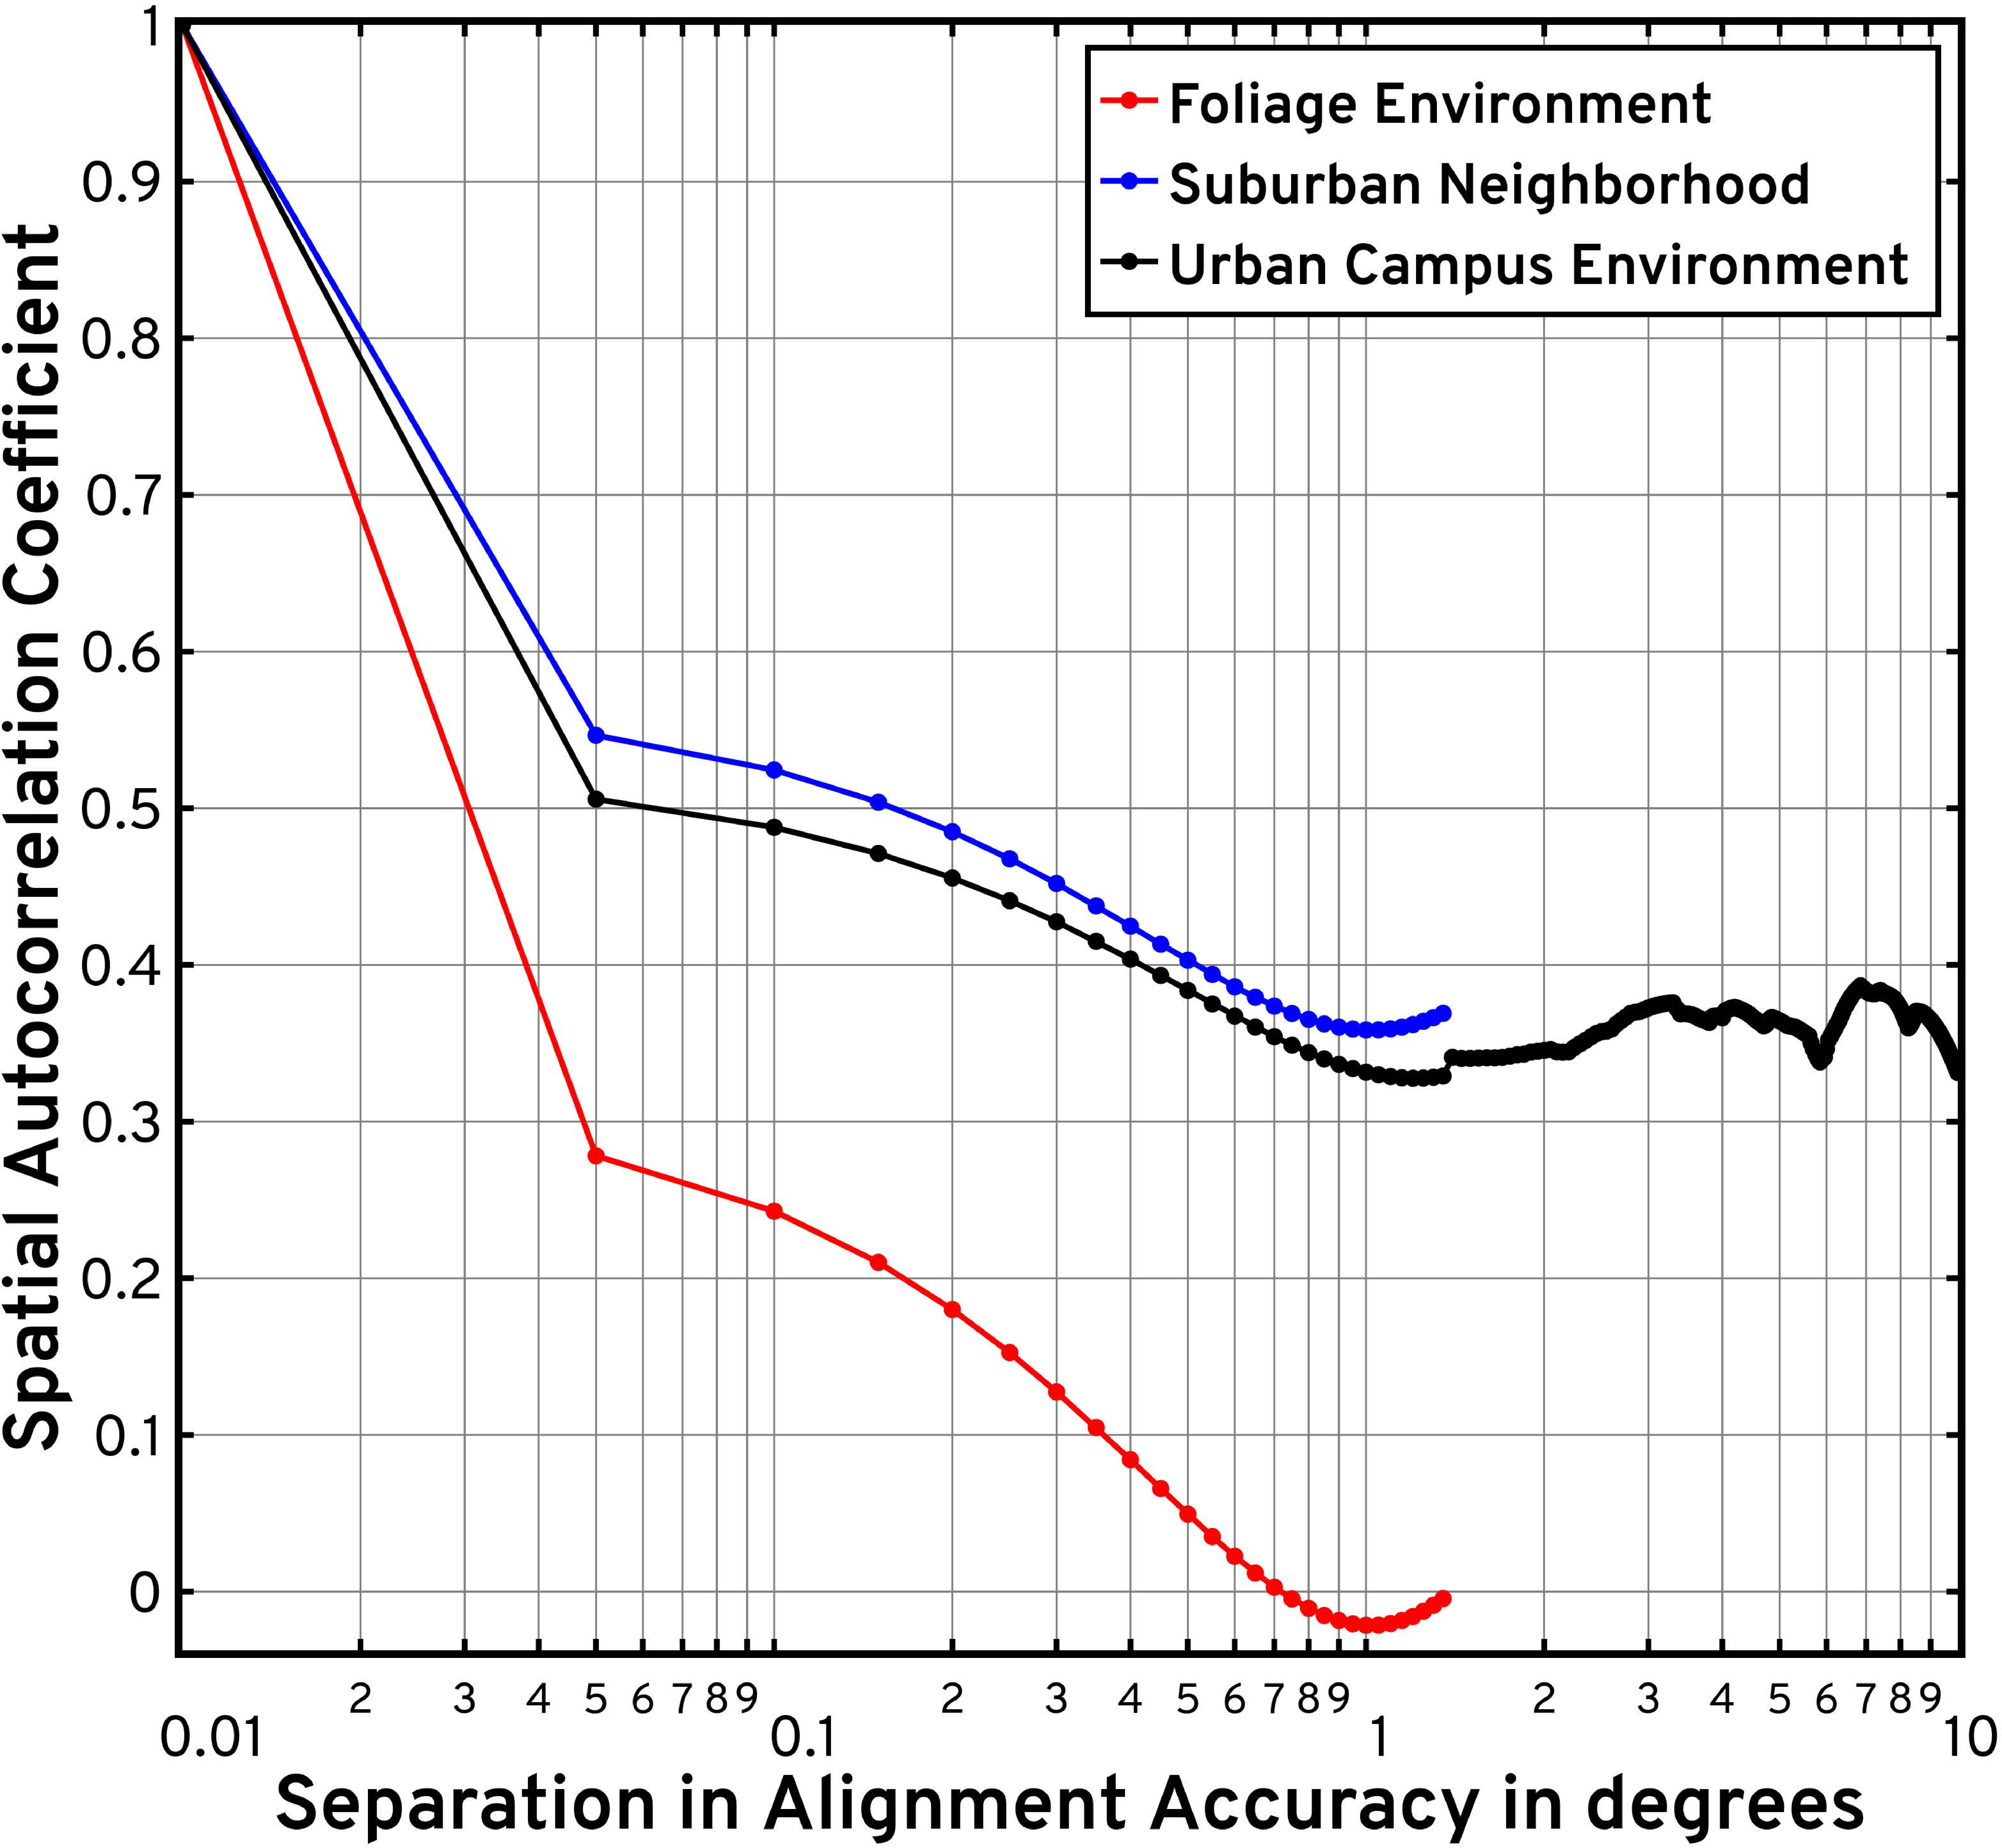
\includegraphics[width=0.95\linewidth]{figs/spatial_consistency_vs_alignment_accuracy.pdf}
        \caption{Spatial Consistency vs Alignment Accuracy Separation (\href{https://codeocean.com/capsule/9545863/tree}{CodeOcean}~\cite{CodeOcean}; \href{http://ieee-dataport.org/12580}{DataPort}~\cite{DataPort})}
        \label{F8a}
    \end{subfigure}
    \begin{subfigure}{0.4975\linewidth}
        \centering
        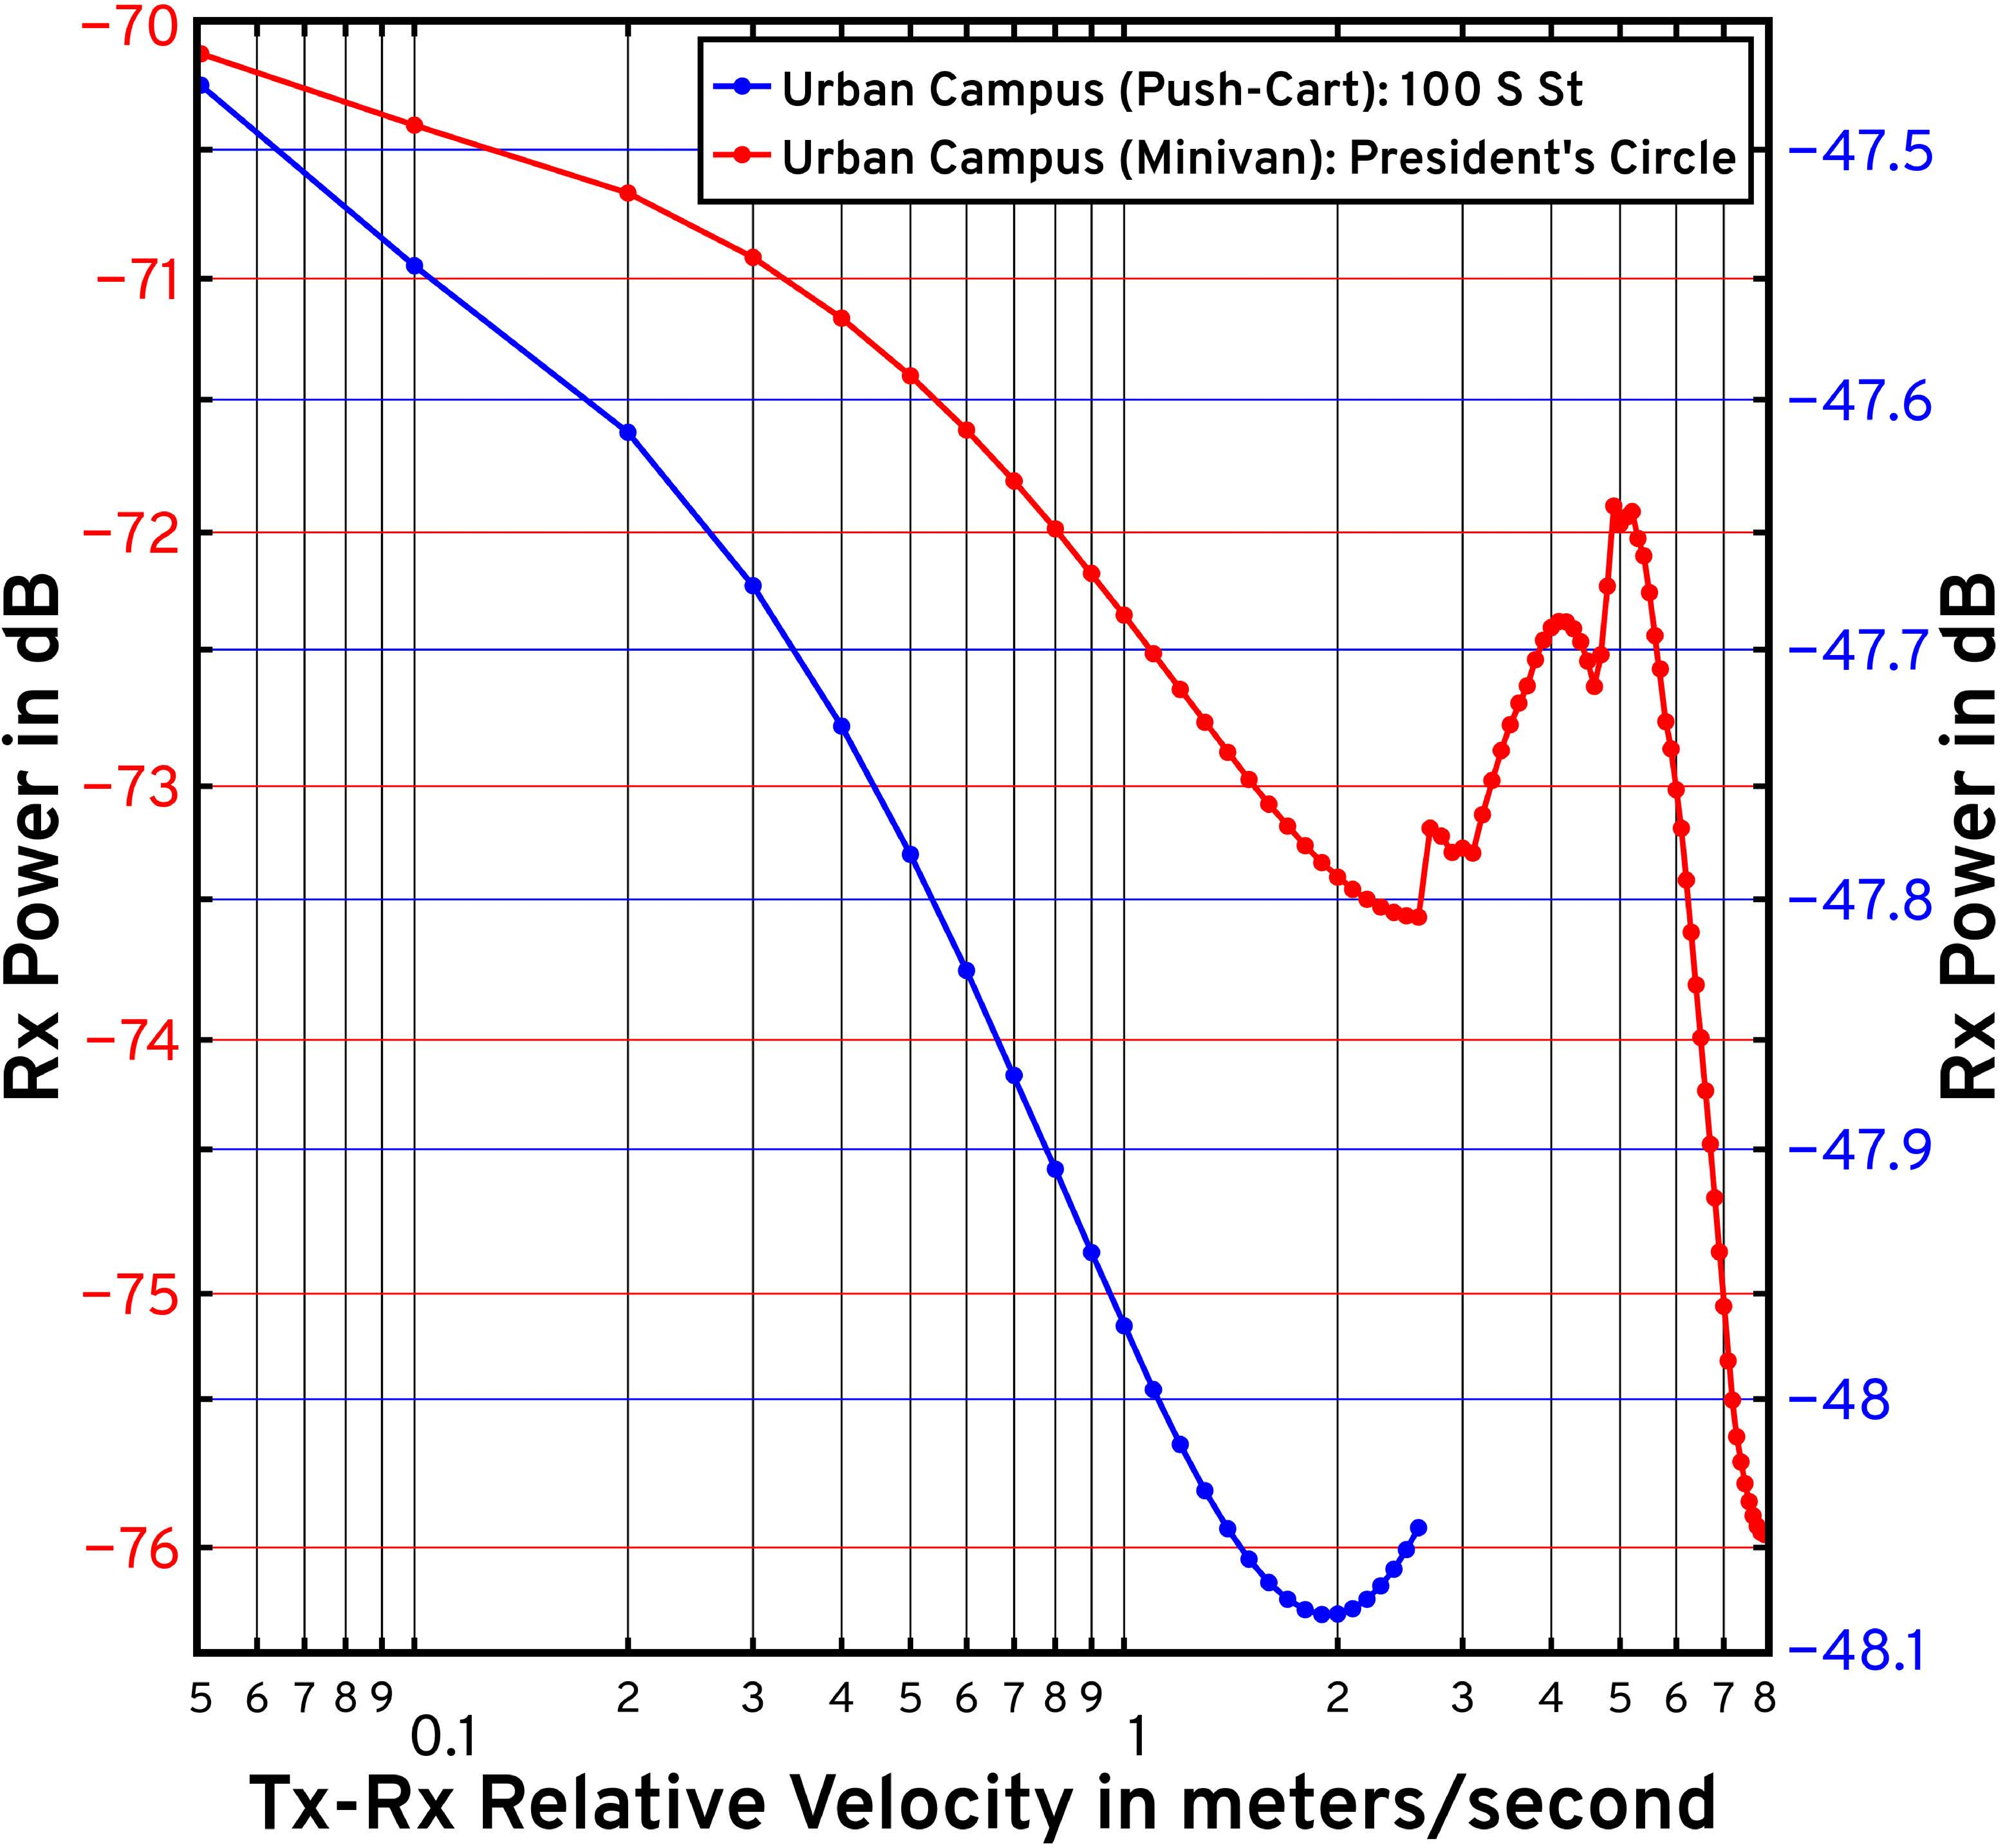
\includegraphics[width=0.95\linewidth]{figs/rx_power_vs_velocity.pdf}
        \caption{Rx Power vs Relative Velocity (\href{https://codeocean.com/capsule/9545863/tree}{CodeOcean}~\cite{CodeOcean}; \href{http://ieee-dataport.org/12580}{DataPort}~\cite{DataPort})}
        \label{F8b}
    \end{subfigure}
    \vspace{-5mm}
    \caption{A plot of the spatial autocorrelation coefficient vs separation in alignment accuracy, i.e., $\rho(\Delta \phi)$ vs log alignment accuracy (in degrees) (a); and a plot of the received signal power (in dB) vs Tx-Rx relative velocity (in meters/second) (b) for urban campus routes: $100$ S St (cart) and President's Circle (van).}
    \vspace{-6mm}
    \label{F8}
\end{figure*}
\indent{For} the MPC at delay bin $\tau_{l}{\in}\boldsymbol{\tau}$, the local amplitude mean (temporal average) across the set of measurements collected at a route configuration index $i \in \mathcal{I}$ is $A_{i}(\tau_{l}) \triangleq \frac{1}{J_{i}}\sum_{j = 1}^{J_{i}}\ A_{i,j}(\tau_{l})$. Let $\mathbf{d}{\triangleq}\{d_{1},d_{2},{\dots},d_{K}\}$ be the Tx-Rx distance bins (quantization of distances) along this route $\mathcal{R}$; similarly, let $\boldsymbol{\phi}{\triangleq}\{\phi_{1},\phi_{2},{\dots},\phi_{M}\}$ denote the Tx-Rx alignment accuracy bins. Then, we define $\mathcal{I}(d_{k}, \phi_{m}) \triangleq \{i \in \mathcal{I}: \norm{\mathbf{x}_{i} - \mathbf{y}_{i}} \approx d_{k}, \phi_{i} \approx \phi_{m}\}$ as the set of route configuration indices for which their Tx-Rx distance belongs to distance bin $d_{k}$ and their Tx-Rx alignment accuracy belongs to alignment bin $\phi_{m}$ (note that, here the bin based quantization is shown with the $\approx$ notation). Next, to study signal decoherence behavior under distance separations, for a route configuration index $i \in \mathcal{I}$ with its Tx-Rx distance in distance bin $d_{k} \in \mathbf{d}$ and Tx-Rx alignment accuracy in alignment bin $\phi_{m} \in \boldsymbol{\phi}$, we define the amplitude sample mean (spatial average) of the MPC at delay bin $\tau_{l} \in \boldsymbol{\tau}$ as $\mu_{i}(\tau_{l}) = \frac{1}{|\mathcal{I}(d_{k}, \phi_{m})|}\sum_{\iota = 1}^{|\mathcal{I}(d_{k}, \phi_{m})|}\ A_{\iota}(\tau_{l})$; similarly, for a route configuration index $i'{\in}\mathcal{I}$ with Tx-Rx distance in distance bin $d_{k'} \in \mathbf{d}$ and Tx-Rx alignment accuracy in alignment bin $\phi_{m} \in \boldsymbol{\phi}$, we define the amplitude sample mean (spatial average) of the MPC at delay bin $\tau_{l} \in \boldsymbol{\tau}$ as $\mu_{i'}(\tau_{l}) = \frac{1}{|\mathcal{I}(d_{k'}, \phi_{m})|}\sum_{\iota = 1}^{|\mathcal{I}(d_{k'}, \phi_{m})|}\ A_{\iota}(\tau_{l})$. Note that the sets used to compute these amplitude sample means for $i, i' \in \mathcal{I}$ could potentially differ only in their Tx-Rx distance bin, i.e., consistent with the condition~\eqref{E}, they should belong to the same alignment accuracy bin. In a similar vein, consistent with the condition~\eqref{Ea}, for alignment accuracy separations, the amplitude sample means $\mu_{i}(\tau_{l})$ and $\mu_{i'}(\tau_{l})$ involve index sets that could potentially differ only in their Tx-Rx alignment accuracy bins, i.e., they should belong to the same distance bin. Thus, using these definitions of the amplitude sample means and with the index sets~\eqref{E} and~\eqref{Ea} serving as evaluation conditions, we define the spatial autocorrelation coefficient $\rho$ under a separation in distance $\Delta d$ and a separation in alignment accuracy $\Delta \phi$ as depicted by Eq.~\eqref{SC} and Eq.~\eqref{SC2}.\\
\begin{table*}
    \centering
    \begin{minipage}{0.75\textwidth}
        \begin{align}\label{SC}
            &\rho(\Delta d) = \frac{\frac{1}{|\mathcal{I}(\Delta d)|}\sum_{(i,i') \in \mathcal{I}(\Delta d)}\Bigg[\sum_{l = 1}^{L}\bigg(\Big(A_{i}(\tau_{l}) - \mu_{i}(\tau_{l})\Big)\Big(A_{i'}(\tau_{l}) - \mu_{i'}(\tau_{l})\Big)\bigg)\Bigg]}{\frac{1}{|\mathcal{I}|}\sum_{i \in \mathcal{I}}\bigg[\sum_{l = 1}^{L}\Big(A_{i}(\tau_{l}) - \mu_{i}(\tau_{l})\Big)^{2}\bigg]},\\
            &\rho(\Delta \phi) = \frac{\frac{1}{|\mathcal{I}(\Delta \phi)|}\sum_{(i,i') \in \mathcal{I}(\Delta \phi)}\Bigg[\sum_{l = 1}^{L}\bigg(\Big(A_{i}(\tau_{l}) - \mu_{i}(\tau_{l})\Big)\Big(A_{i'}(\tau_{l}) - \mu_{i'}(\tau_{l})\Big)\bigg)\Bigg]}{\frac{1}{|\mathcal{I}|}\sum_{i \in \mathcal{I}}\bigg[\sum_{l = 1}^{L}\Big(A_{i}(\tau_{l}) - \mu_{i}(\tau_{l})\Big)^{2}\bigg]}.\label{SC2}
        \end{align}
    \end{minipage}
    \vspace{-6mm}
\end{table*}
\indent{As} a result of the framework described above, Fig.~\ref{F7b} illustrates the spatial consistency curves as a function of the separations in distance for the urban campus, suburban neighborhood, and foliage environment routes. In this plot, we observe decreasing correlation trends between recorded power delay profile samples for increasing distance separation. Fig.~\ref{F8a} depicts the variation of the spatial autocorrelation coefficient under increasing levels of misalignment between the Tx and Rx antennas while traversing the urban campus, suburban neighborhood, and foliage environment routes. We observe rapid decorrelation across the evaluated samples even at small amounts of misalignment, highlighting the highly directional characteristics of our WR-$28$ horn antennas, and illustrating the need for accurate beam-steering in mmWave V$2$X networks. Note that, in Fig.~\ref{F7b} and Fig.~\ref{F8a}, the channel does not get fully decorrelated since in our beam-steered setup, the line-of-sight component always remains significant. Lastly, Fig.~\ref{F8b} depicts the received signal power at the Rx for changes in the Tx-Rx relative velocity around the urban campus routes onsite wherein the Rx is mounted either on a push-cart ($100$ S St, \SI{0}{}-\SI{5}{mph}) or on a minivan (President's Circle, \SI{0}{}-\SI{18}{mph}). Here, we observe considerable drops in received power for minor velocity variations due to response latencies and misalignments introduced into our mechanical beam-steering platform as the Rx is driven away from the Tx, reiterating the need for accurate and responsive beam-steering designs for mmWave communications in V$2$X applications.
\begin{figure*} [t]
    \centering
    \begin{subfigure}{0.4965\linewidth}
        \centering
        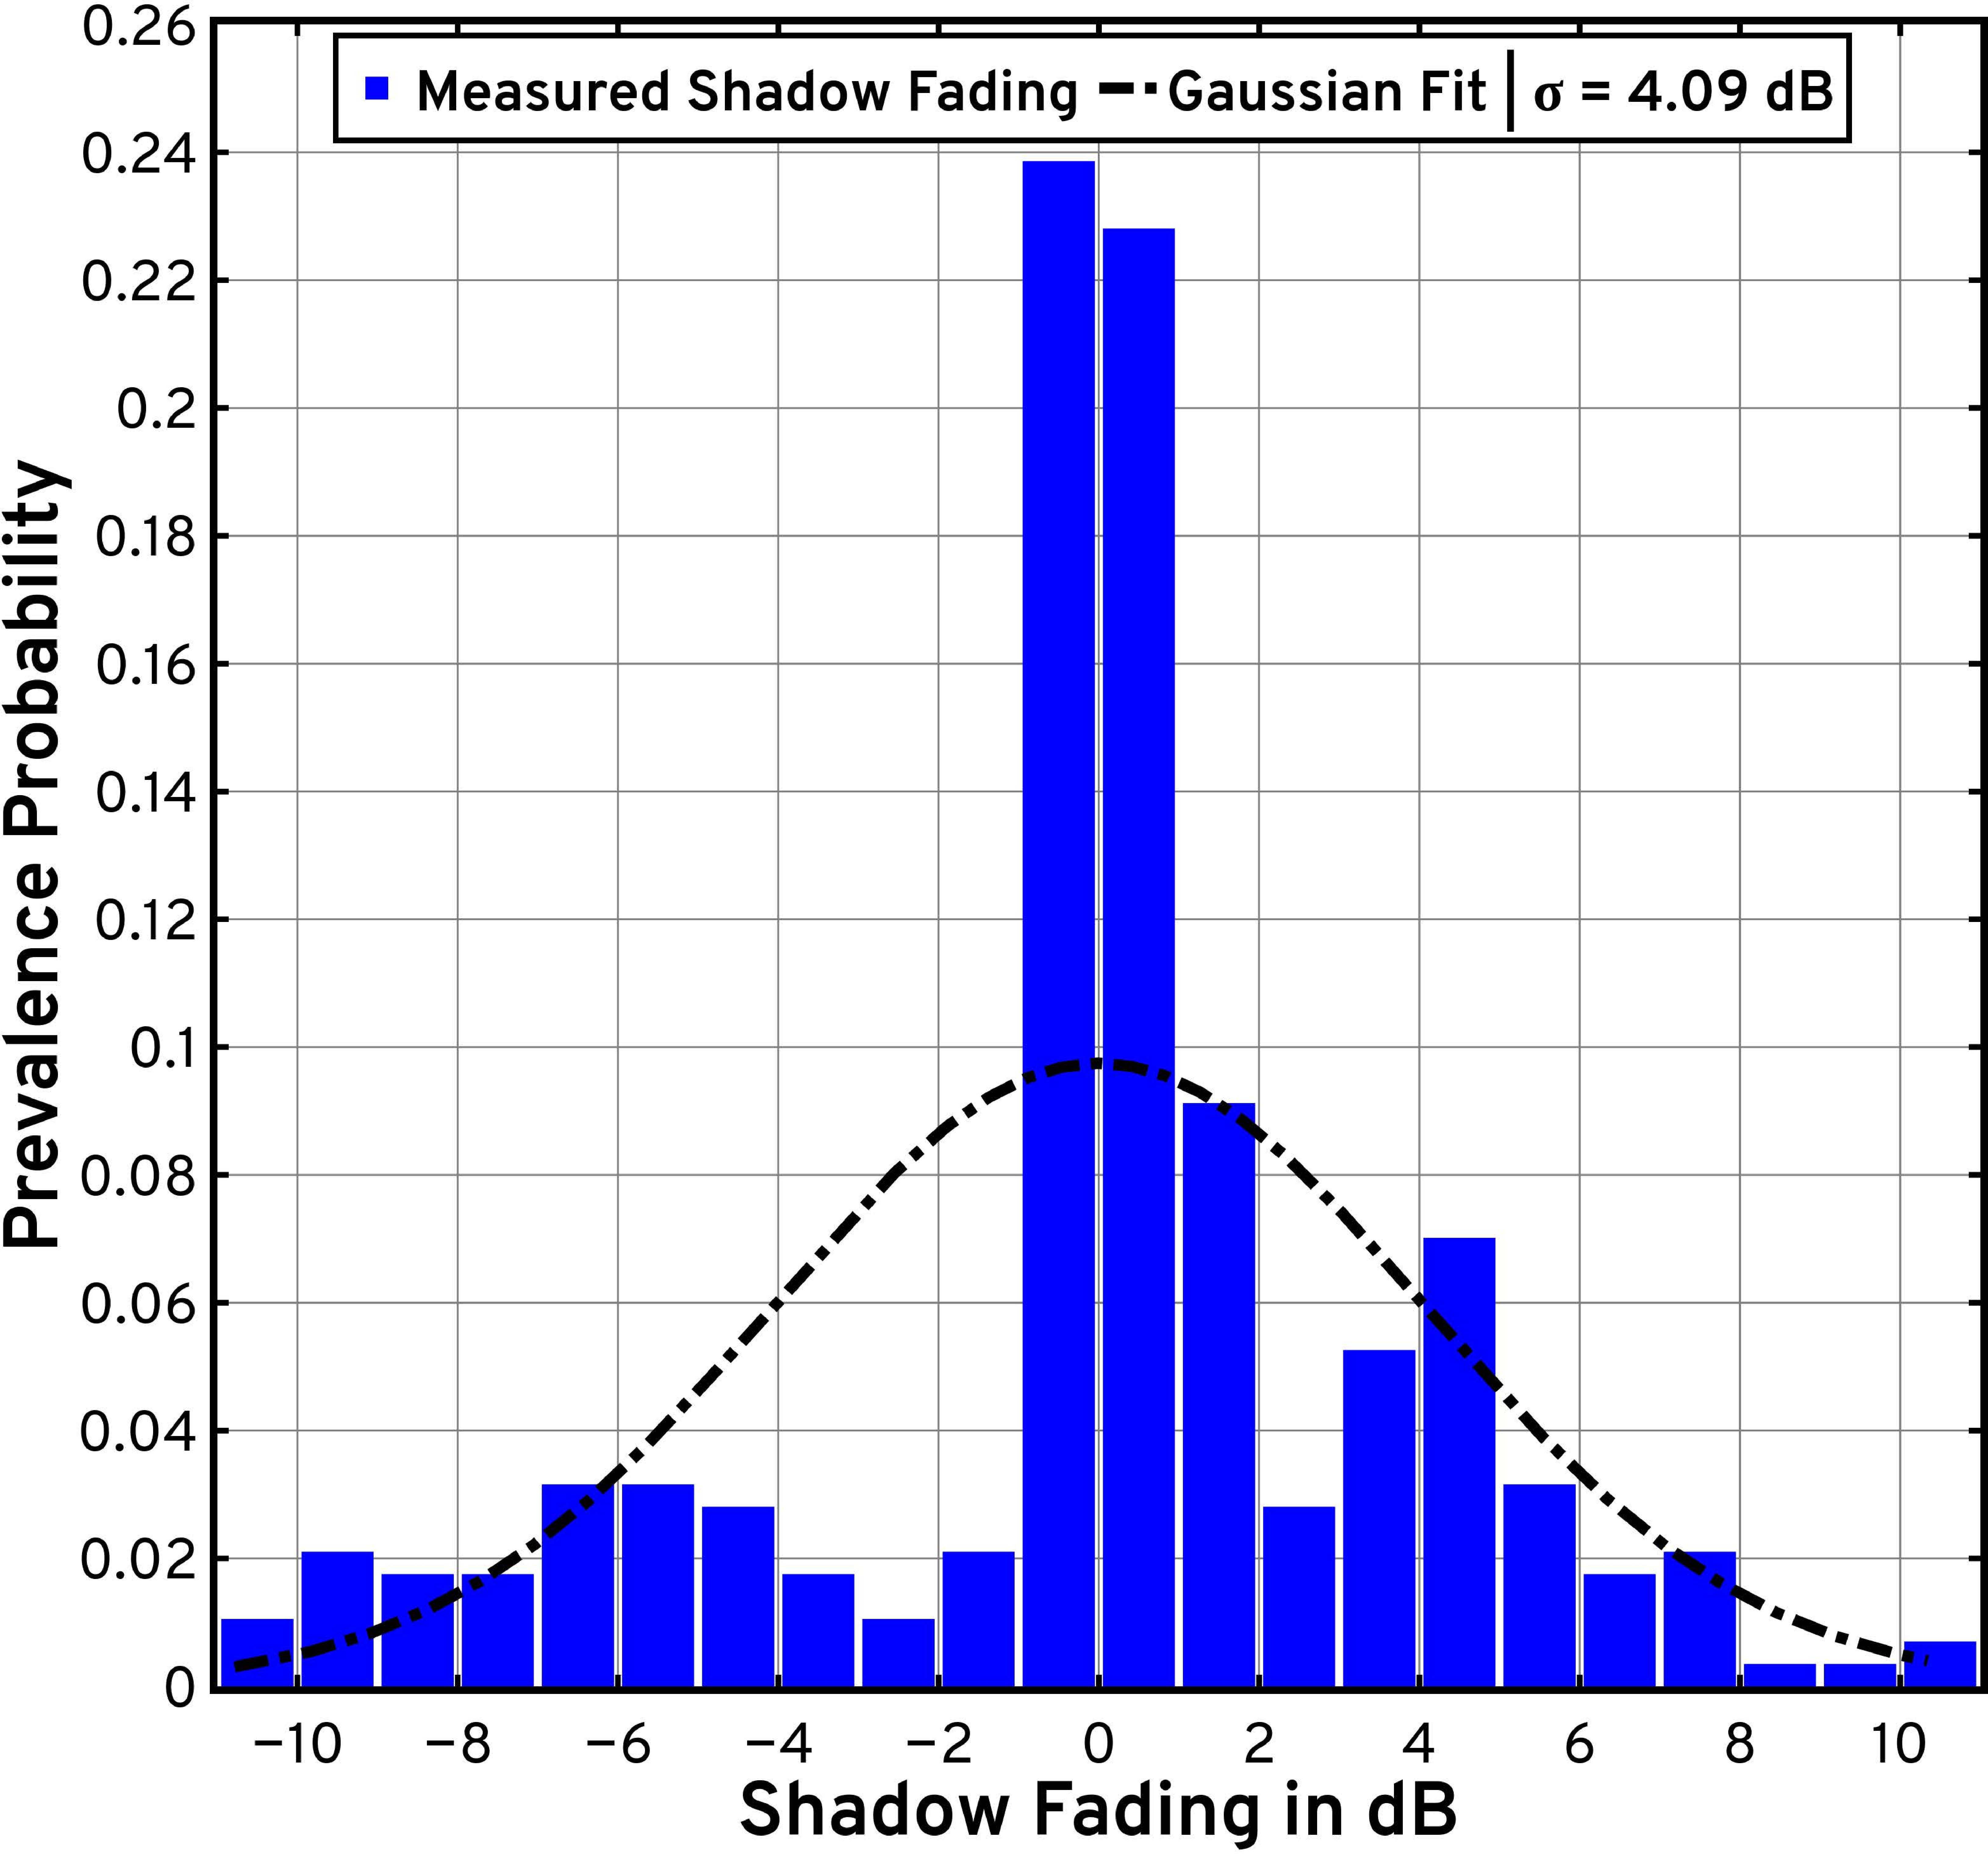
\includegraphics[width=0.95\linewidth]{figs/urban_campus_shadow_fading_1.pdf}
        \caption{Urban Campus: President's Circle (\href{https://codeocean.com/capsule/9545863/tree}{CodeOcean}~\cite{CodeOcean}; \href{http://ieee-dataport.org/12580}{DataPort}~\cite{DataPort})}
        \label{F9a}
    \end{subfigure}
    \begin{subfigure}{0.4935\linewidth}
        \centering
        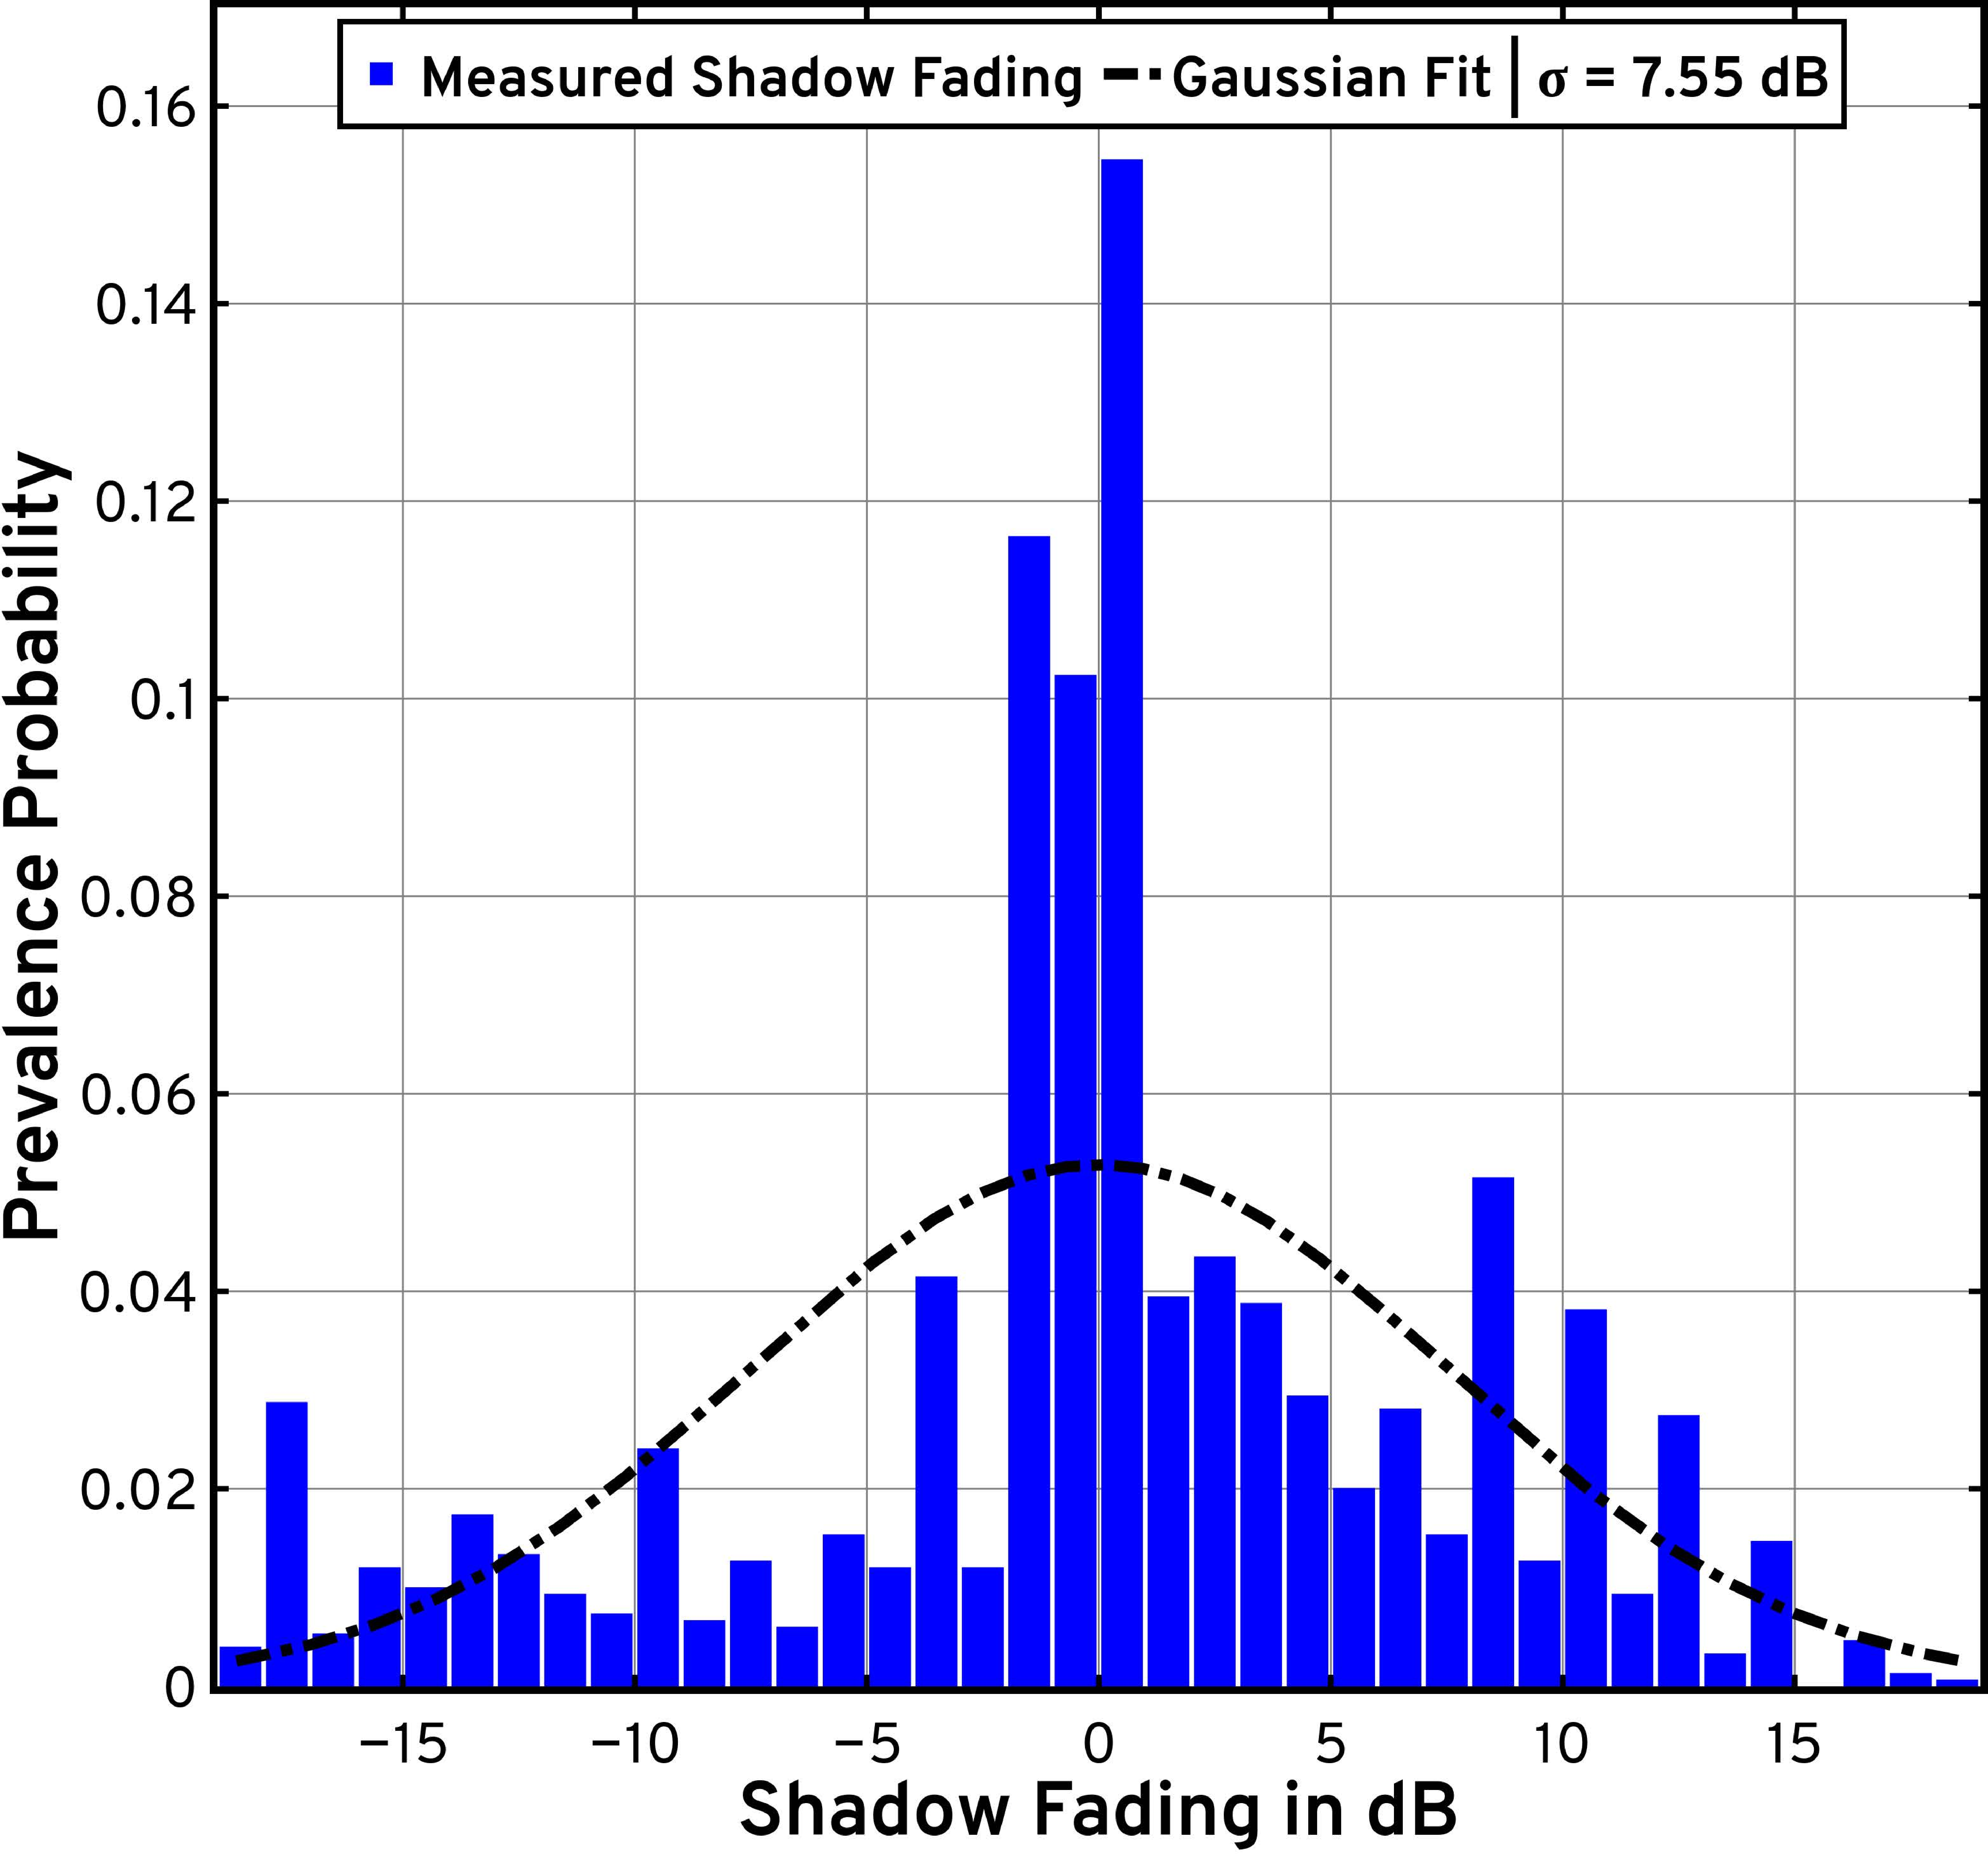
\includegraphics[width=0.95\linewidth]{figs/urban_campus_shadow_fading_2.pdf}
        \caption{Urban Campus: $100$ S St (\href{https://codeocean.com/capsule/9545863/tree}{CodeOcean}~\cite{CodeOcean}; \href{http://ieee-dataport.org/12580}{DataPort}~\cite{DataPort})}
        \label{F9b}
    \end{subfigure}
    \vspace{-5mm}
    \caption{The histograms and Gaussian fits for the shadowing (in dB) of mmWave signals along urban campus routes: President's Circle (a) and $100$ S St (b).}
    \vspace{-4mm}
    \label{F9}
\end{figure*}
\\\noindent{\textbf{Shadowing and Dynamic Blockages}}: The shadowing plots for the two urban campus routes, i.e., President's Circle (Rx on a minivan) and $100$ S St (Rx on a push-cart), are depicted in Fig.~\ref{F9a} and Fig.~\ref{F9b}. Averaging out the effects of multipath fading across several measurements over a \SI{1}{\meter} distance resolution~\cite{Averaging_Threshold}, these plots depict the histograms of the deviations of the measured pathloss values from those provided by the linear models fitted to our measurements in Fig.~\ref{F7a}; upon visualizing these histograms for the two urban campus routes (dominated by tall buildings), we fit Gaussian distribution curves to obtain the log-normal shadow fading distributions typically seen in the state-of-the-art~\cite{DopplerHST}. Herein, as is evident from the structural profiles of the two routes (see Fig.~\ref{F5a} and Fig.~\ref{F5b}), we observe that the urban campus route around $100$ S St exhibits a larger shadowing impact ($\sigma{=}$\SI{7.55}{\deci\bel}) relative to that around President's Circle ($\sigma{=}$\SI{4.09}{\deci\bel}) due to higher obstacle density around $100$ S St.
\begin{figure*} [t]
    \centering
    \begin{subfigure}{0.5\linewidth}
        \centering
        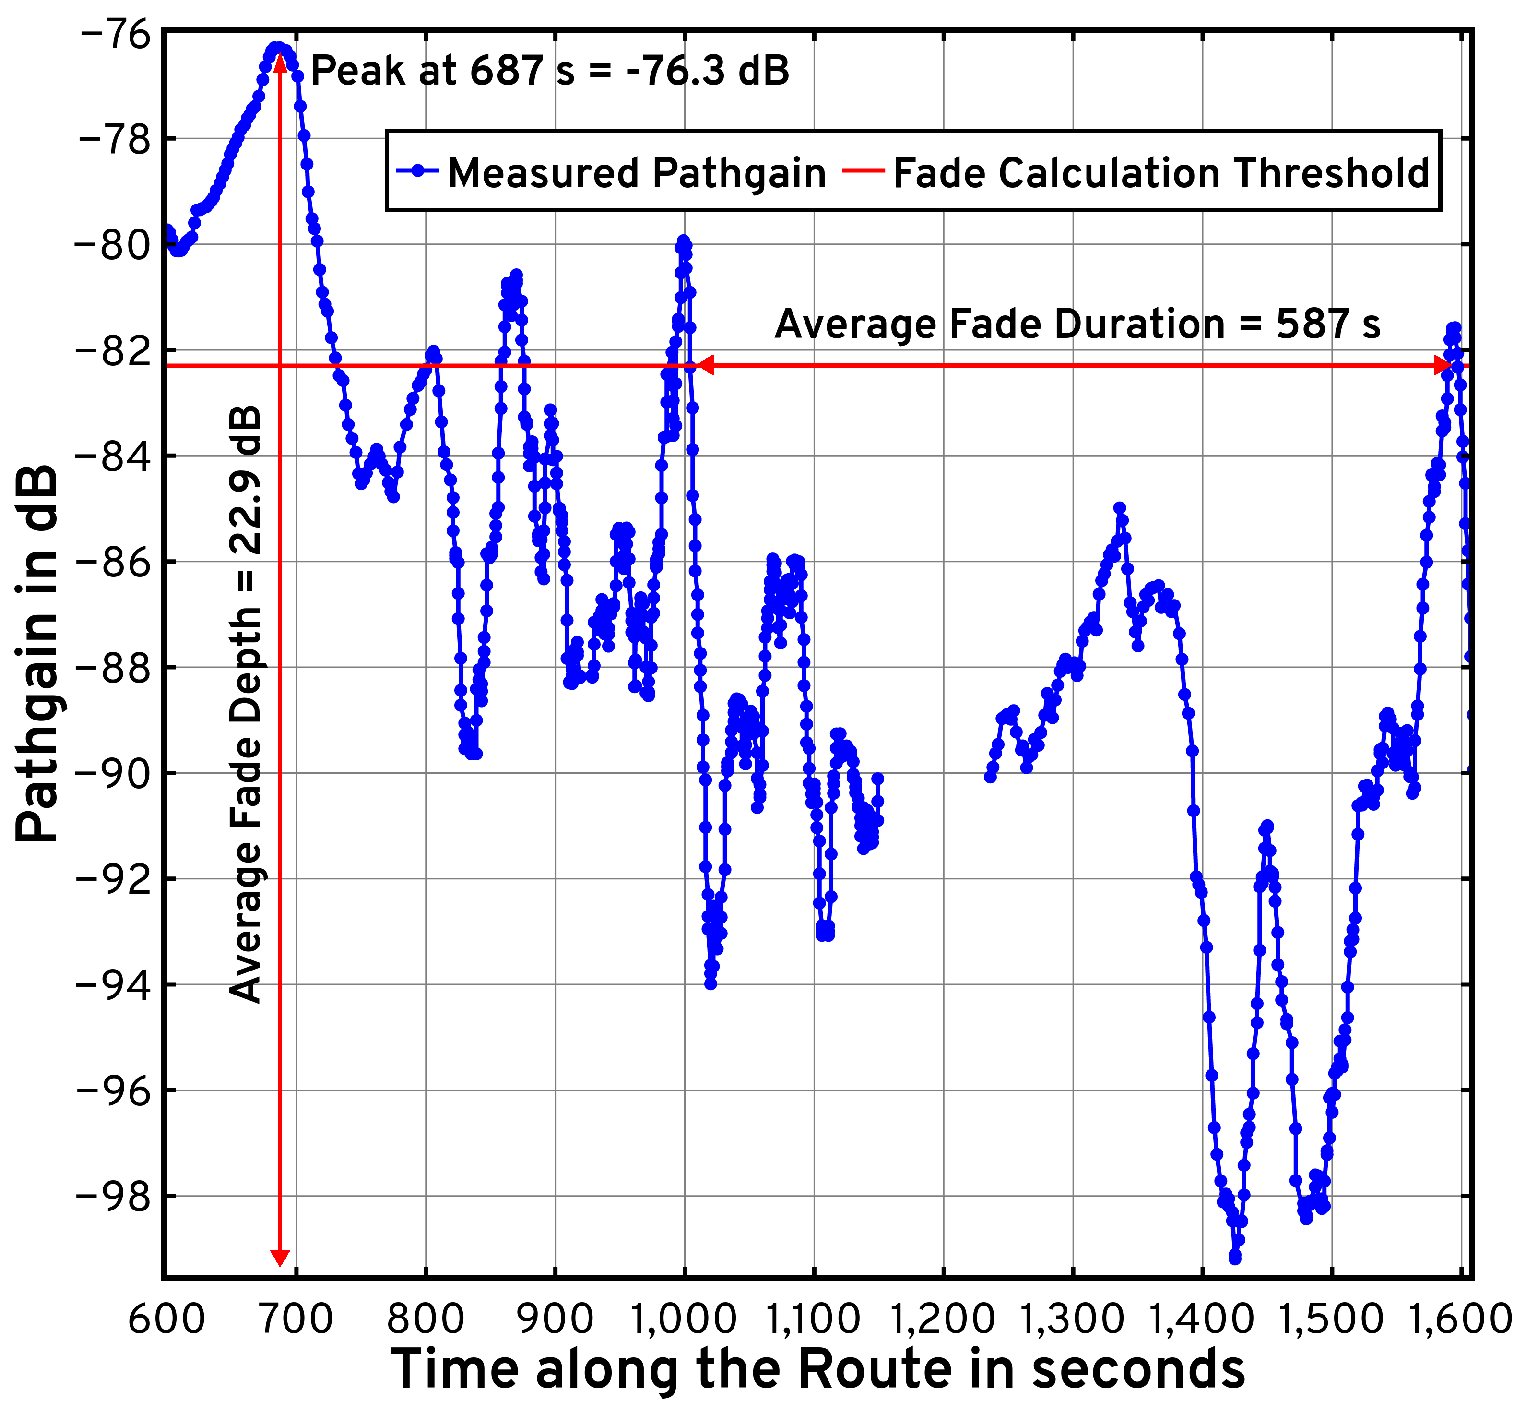
\includegraphics[width=0.95\linewidth]{figs/urban_campus_pathgain_vs_time_gap_annotated.pdf}
        \caption{Urban Campus: $100$ S St (\href{https://codeocean.com/capsule/9545863/tree}{CodeOcean}~\cite{CodeOcean}; \href{http://ieee-dataport.org/12580}{DataPort}~\cite{DataPort})}
        \label{F10a}
    \end{subfigure}
    \begin{subfigure}{0.49\linewidth}
        \centering
        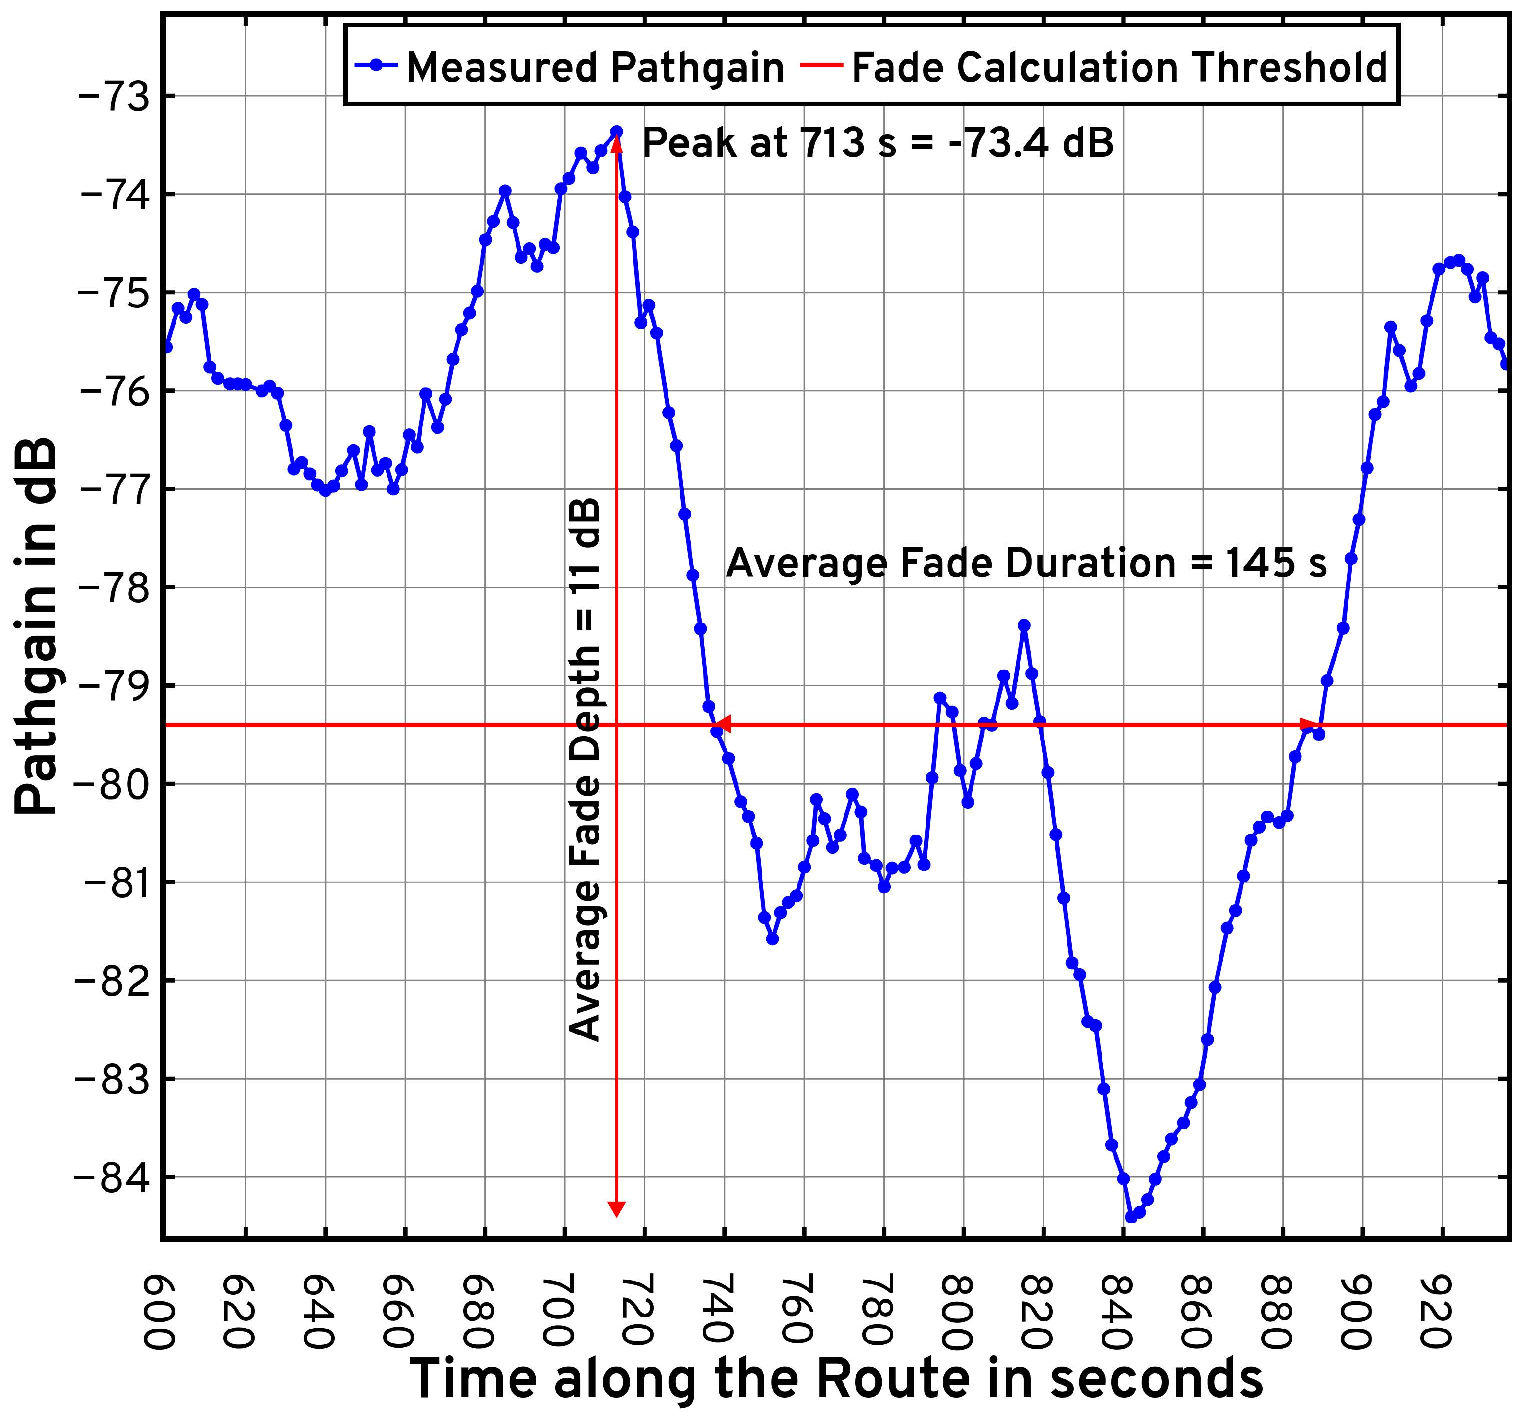
\includegraphics[width=0.95\linewidth]{figs/suburban_pathgain_vs_time_annotated.pdf}
        \caption{Suburban Neighborhood: S Wolcott St (\href{https://codeocean.com/capsule/9545863/tree}{CodeOcean}~\cite{CodeOcean}; \href{http://ieee-dataport.org/12580}{DataPort}~\cite{DataPort})}
        \label{F10b}
    \end{subfigure}
    \vspace{-5mm}
    \caption{The plots depicting fading trends (pathgain in dB vs time in seconds) exhibited by \SI{28}{\giga\hertz} signals for routes involving static (buildings) and dynamic blockages (pedestrians, moving/parked vehicles): urban campus route around $100$ S St (a) and suburban neighborhood route around S Wolcott St (b).}
    \vspace{-4.093mm}
    \label{F10}
\end{figure*}
\\\indent{Moreover}, the small-scale fading studies of \SI{28}{\giga\hertz} signals in V$2$X scenarios vis-à-vis the average fade depth and duration metrics, along routes dominated by static (buildings) and dynamic (pedestrians, moving/parked vehicles) blockages, are depicted in Fig.~\ref{F10a} and Fig.~\ref{F10b}. In V$2$X use cases, these pathgain vs route time plots enable us to gather insights about the attenuations introduced into the mmWave signal path due to obstacles, viz., static/stationary obstacles and dynamic/transient obstacles (which move in and out of the signal path quickly). Studying the fade depth and duration metrics in Fig.~\ref{F10a} and Fig.~\ref{F10b}, we note that the urban campus route around $100$ S St (Rx on a push-cart) exhibits a larger signal fade (${\approx}$\SI{23}{\deci\bel}) over a longer duration relative to the suburban neighborhood route around S Wolcott St (Rx on a push-cart, fade of \SI{11}{\deci\bel}). This is due to two reasons: a) a higher static obstacle density around the $100$ S St route not only causes a larger signal fade (due to blockages by tall buildings) for a longer duration (in the order of hundreds of seconds), but also results in frequent drops in Rx power of relatively longer durations (in the order of a tens of seconds) as considerably many more moving/parked vehicles enter into and exit out of the signal path with appreciable frequency; b) the suburban neighborhood route around S Wolcott St had a lower building density (see Figs.~\ref{F5b} and~\ref{F6b}) and a relatively negligible vehicular density (\SIrange{1}{2}{} parked vehicles at route time ${\approx}$\SI{840}{\second}), but instead had low frequency pedestrian traffic, thereby resulting in the signals here experiencing smaller and infrequent fades over shorter durations. Also, evaluating these average fade depth and duration metrics against those reported by the D$2$D mmWave channel model~\cite{D2DHumanBlockage}, we note that, while the D$2$D model does not provide these fade metrics for vehicular traffic, the average fade depth reported by it for the obstructed signal attenuated by transient pedestrian traffic (as seen around S Wolcott St) is between \SI{20}{}-\SI{25}{\deci\bel}, which is significantly higher than that seen in Fig.~\ref{F10b} (\SI{11}{\deci\bel}). In the next section, using the MPCs and their parameters (extracted via the SAGE algorithm detailed earlier), we present multipath clustering evaluations which includes cluster arrival and decay characteristics, RMS delay and direction spreads, along with empirical validations of statistical mmWave channel models.
\begin{figure*} [t]
    \centering
    \begin{subfigure}{0.494\linewidth}
        \centering
        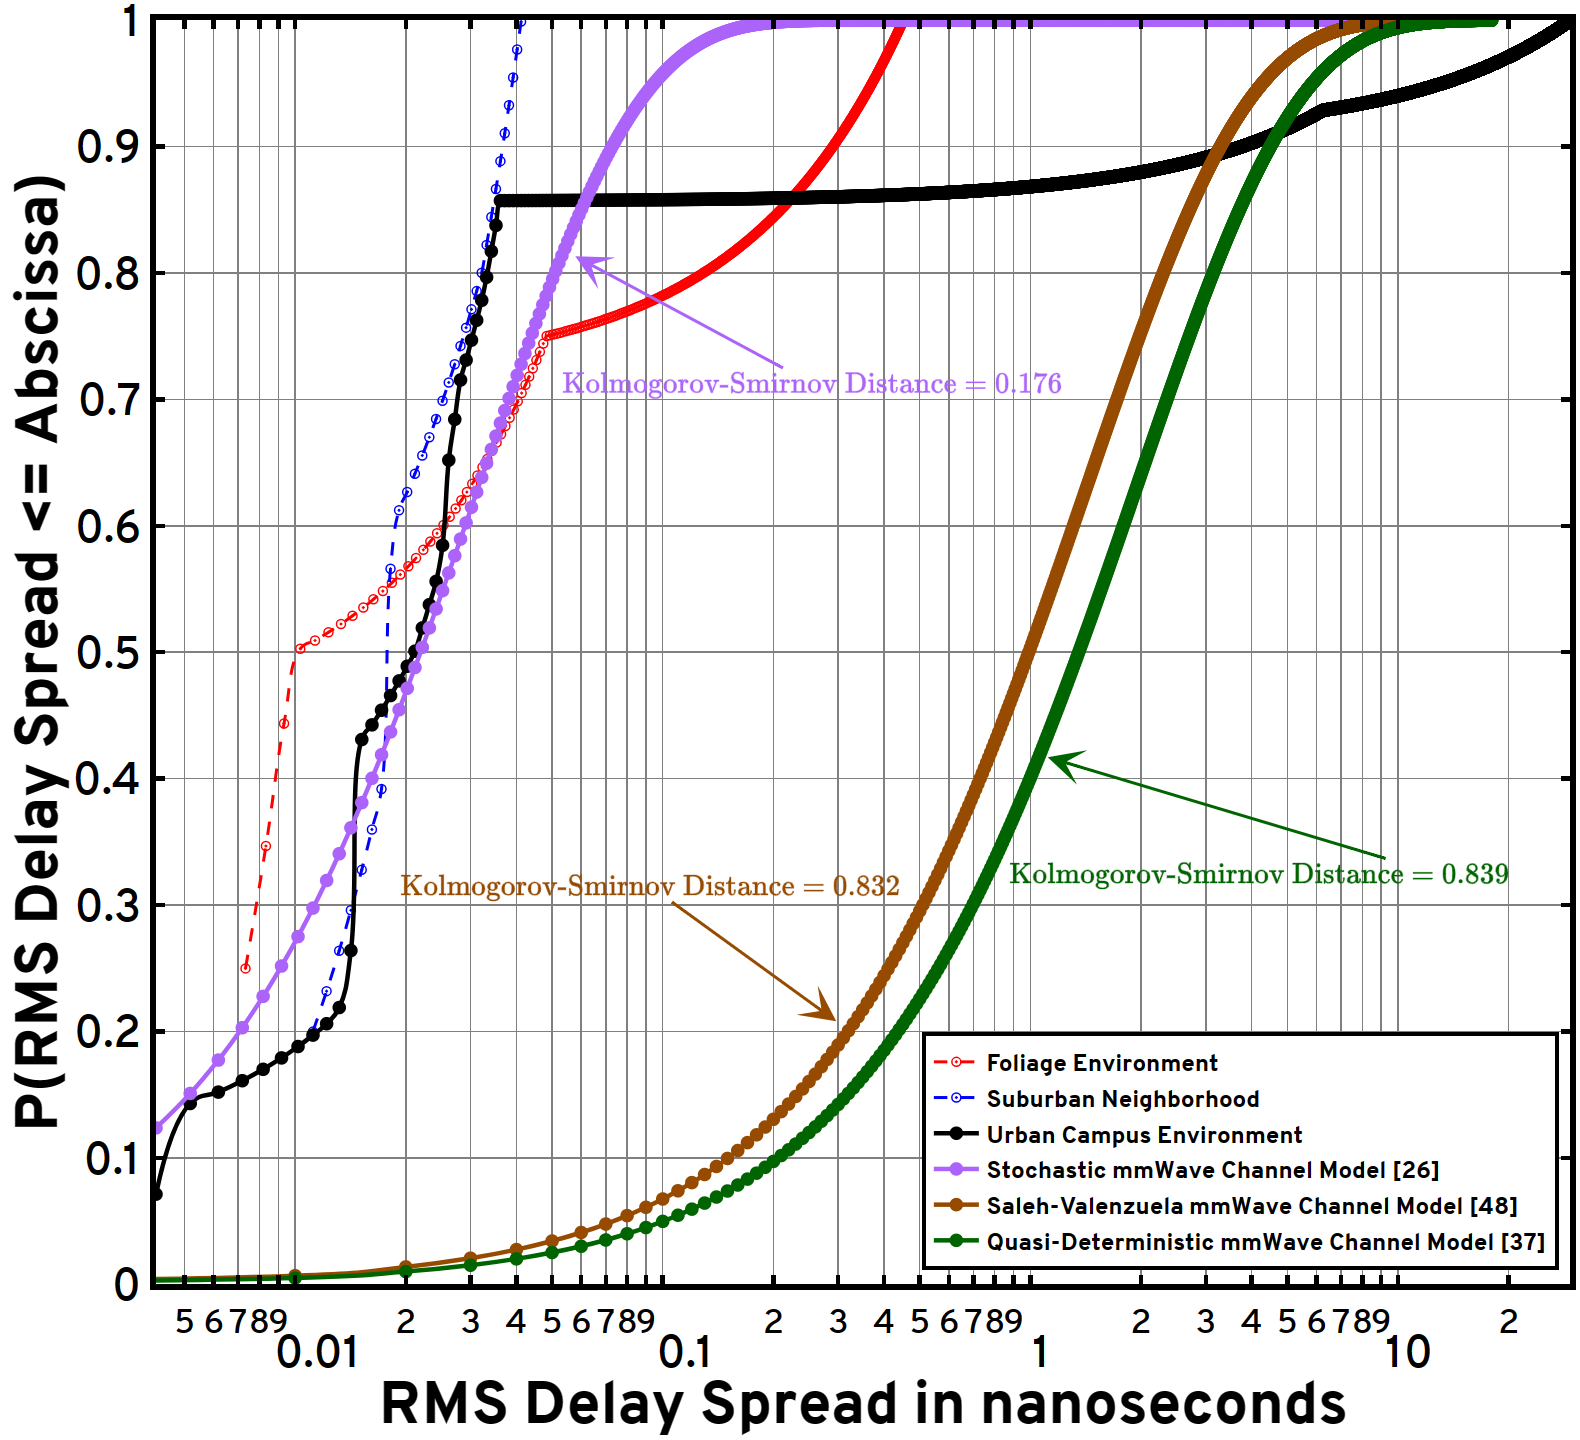
\includegraphics[width=0.97\linewidth]{figs/rms_delay_spread.png}
        \caption{RMS Delay Spread CDFs (\href{https://codeocean.com/capsule/9545863/tree}{CodeOcean}~\cite{CodeOcean}; \href{http://ieee-dataport.org/12580}{DataPort}~\cite{DataPort})}
        \label{F11a}
    \end{subfigure}
    \begin{subfigure}{0.496\linewidth}
        \centering
        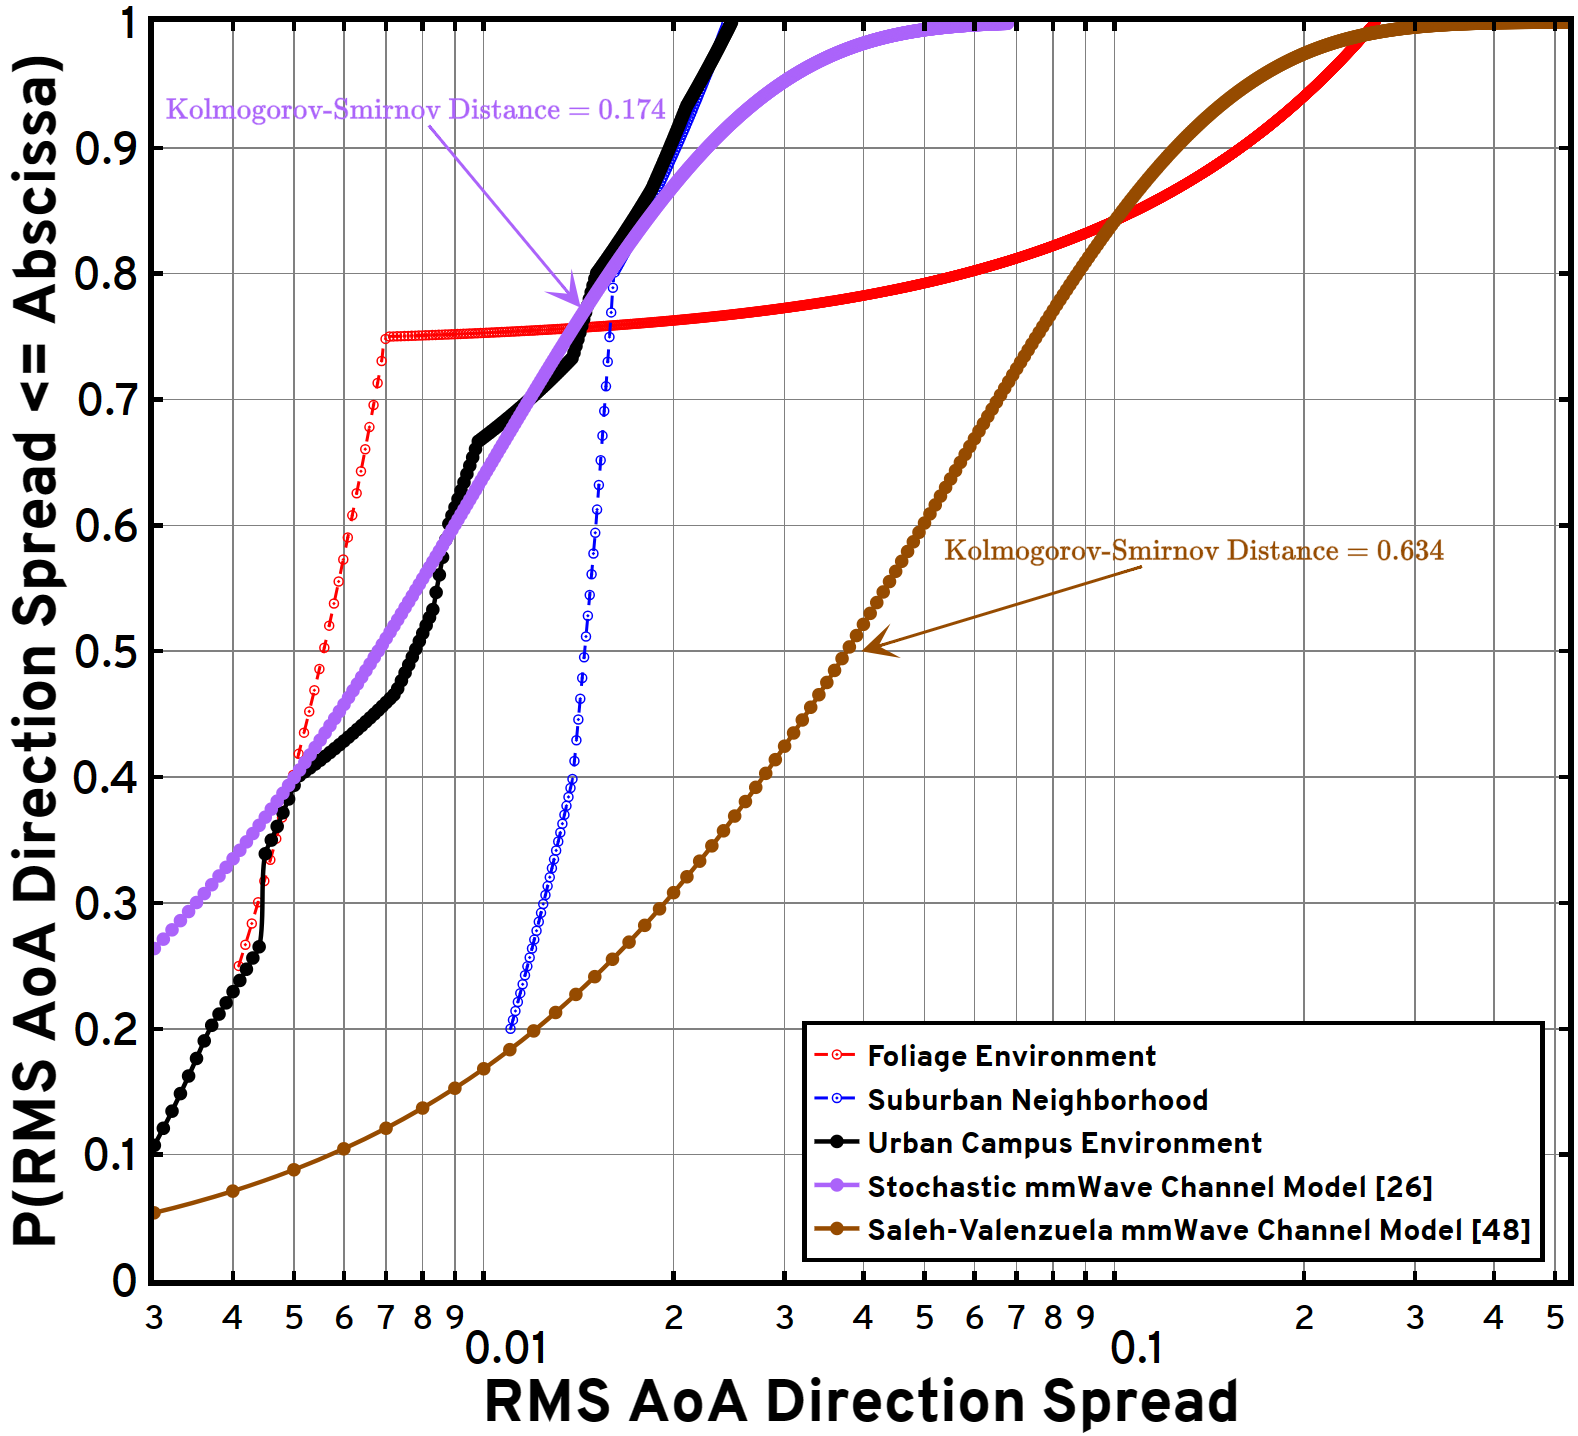
\includegraphics[width=0.97\linewidth]{figs/rms_aoa_direction_spread.png}
        \caption{RMS AoA Direction Spread CDFs (\href{https://codeocean.com/capsule/9545863/tree}{CodeOcean}~\cite{CodeOcean}; \href{http://ieee-dataport.org/12580}{DataPort}~\cite{DataPort})}
        \label{F11b}
    \end{subfigure}
    \vspace{-5mm}
    \caption{The CDFs of the RMS delay spreads (in nanoseconds) (a) and the RMS AoA direction spreads (b), derived from our measurements for the urban campus route around $100$ S St (Rx on a push-cart), the suburban neighborhood route around S Wolcott St (Rx on a push-cart), and the foliage dominated route around the Olpin Union building (Rx on a push-cart). These plots also involve the CDFs derived from the SV~\cite{SV_Molisch}, QD~\cite{QDC_NIST}, and stochastic~\cite{Indoor60G} models.}
    \vspace{-6mm}
    \label{F11}
\end{figure*}
\vspace{-3mm}

% Numerical evaluations II: Multipath clustering and Channel model validations
\section{Multipath Clustering and Channel Modeling}\label{S5}
In this section, using the MPCs extracted via the SAGE algorithm~\cite{SAGE}, we outline our multipath clustering studies involving cluster inter-arrival times, cluster decay attributes, and RMS delay and direction spreads. Also, to evaluate our measurements against the state-of-the-art, we employ the Kolmogorov-Smirnov statistic to facilitate experimental validations of widely used mmWave channel models (SV~\cite{SV_Molisch}, QD~\cite{QDC_NIST}, and stochastic~\cite{Indoor60G}) by providing a measure of the \emph{goodness of fit} between the empirical CDFs and those obtained from these statistical/parameterized mmWave channel models.\\
\indent{Fig.~\ref{F11a}} illustrates the RMS delay spread characteristics of \SI{28}{\giga\hertz} signals, when the Tx is affixed atop the William Browning building and the Rx traverses unplanned vehicular routes around the urban campus, suburban neighborhood, and foliage environments. Herein, the RMS delay spread metric $\sigma_{\tau}$ is computed according to the following relationship~\cite{Indoor60G}:
\vspace{1.8mm}
\begin{align}\label{RMS_DS}
    \sigma_{\tau} = \sqrt{\frac{\sum_{\tau}P_{h}(\tau)\tau^{2}}{\sum_{\tau}P_{h}(\tau)} - \left(\frac{\sum_{\tau}P_{h}(\tau)\tau}{\sum_{\tau}P_{h}(\tau)}\right)^{2}},
\end{align}
where $P_{h}(\tau)$ is the power delay profile (at $\tau$ delay tick) obtained from the channel impulse response $h(\tau)$, i.e., $P_{h}(\tau){=}|h(\tau)|^{2}$. Fig.~\ref{F11a} also illustrates the RMS delay spread CDFs for the SV~\cite{SV_Molisch}, QD~\cite{QDC_NIST}, and stochastic~\cite{Indoor60G} mmWave channel models. Here, the Kolmogorov-Smirnov distance $D_{n}{=}\sup_{x}|F_{n}(x){-}F(x)|$ quantifies the statistical separation between the CDF $F_{n}(x)$ obtained from $n$ independent and identically distributed measurement items and the CDF of the reference distribution $F(x)$ (i.e., RMS delay spread CDFs derived from the statistical channel models); note that $x$ here corresponds to an evaluation metric, e.g., RMS delay spreads, RMS direction spreads, and cluster inter-arrival times. Under our Kolmogorov-Smirnov evaluations, the stochastic channel model~\cite{Indoor60G} ($0.176$) demonstrates \emph{a better fit} with our measurements around the urban campus environment, relative to the SV~\cite{SV_Molisch} ($0.832$) and QD~\cite{QDC_NIST} ($0.839$) channel models. Also, observe that the spread of multipath component delays is larger for the urban campus route compared to the suburban and foliage routes, due to the larger Tx-Rx distances involved and a larger number of reflected paths due to a higher building density. Similarly, Fig.~\ref{F11b} depicts the RMS AoA direction spread characteristics of \SI{28}{\giga\hertz} signals in our propagation modeling campaign onsite at the NSF POWDER experimental testbed, along unplanned Rx vehicular routes around the urban campus, suburban neighborhood, and foliage environments. The RMS AoA direction spread metric $\sigma_{\Omega}$ is calculated as~\cite{Indoor60G}
\begin{align}\label{RMS_DirS}
    \sigma_{\Omega} = \sqrt{\sum_{l=1}^{L}|\mathbf{e}(\phi_{l}, \theta_{l}) - \boldsymbol{\mu}_{\Omega}|^{2}P(\phi_{l}, \theta_{l})},
\end{align}
\begin{figure*} [t]
    \centering
    \begin{subfigure}{0.4975\linewidth}
        \centering
        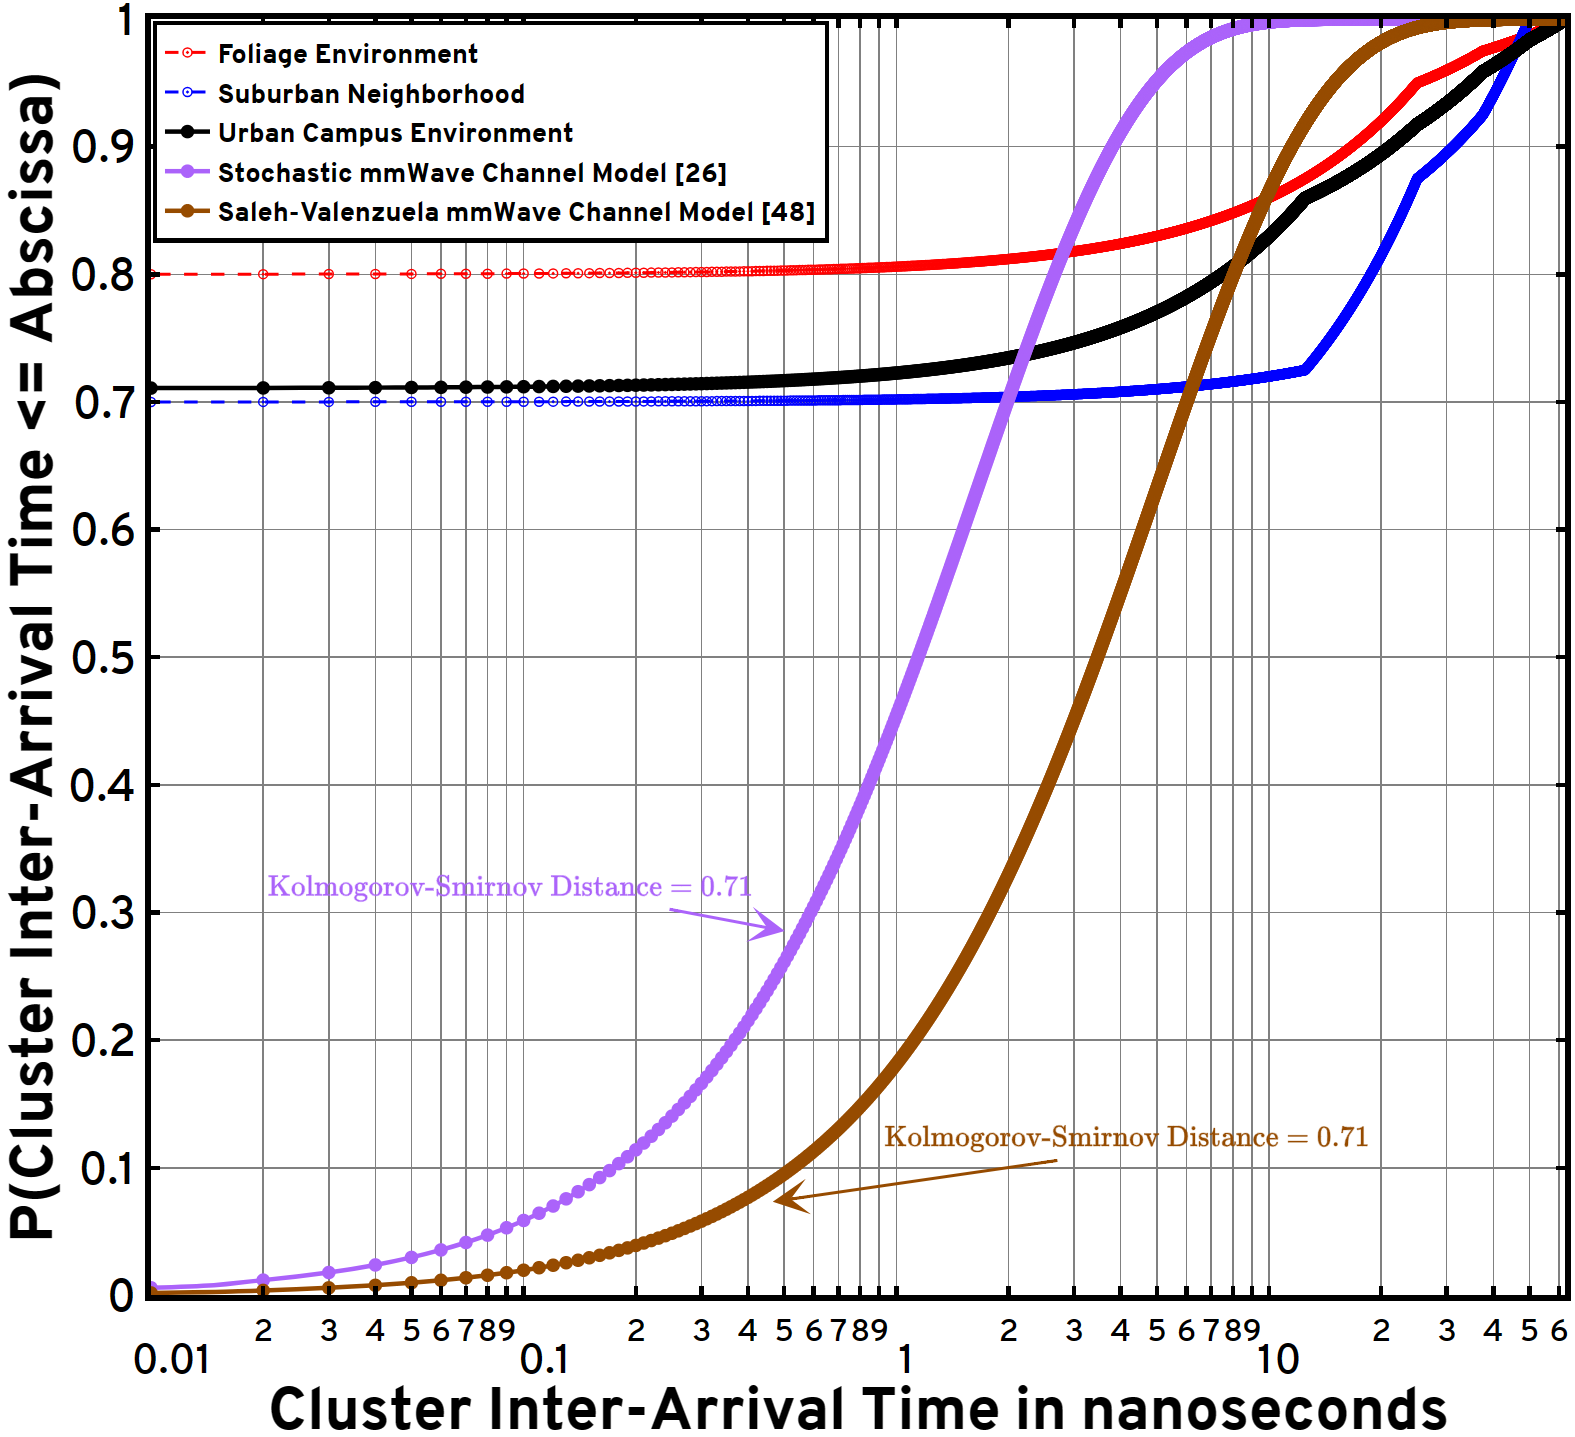
\includegraphics[width=0.97\linewidth]{figs/cluster_arrival_characteristics.png}
        \caption{Cluster Arrival Characteristics (\href{https://codeocean.com/capsule/9545863/tree}{CodeOcean}~\cite{CodeOcean}; \href{http://ieee-dataport.org/12580}{DataPort}~\cite{DataPort})}
        \label{F12a}
    \end{subfigure}
    \begin{subfigure}{0.4925\linewidth}
        \centering
        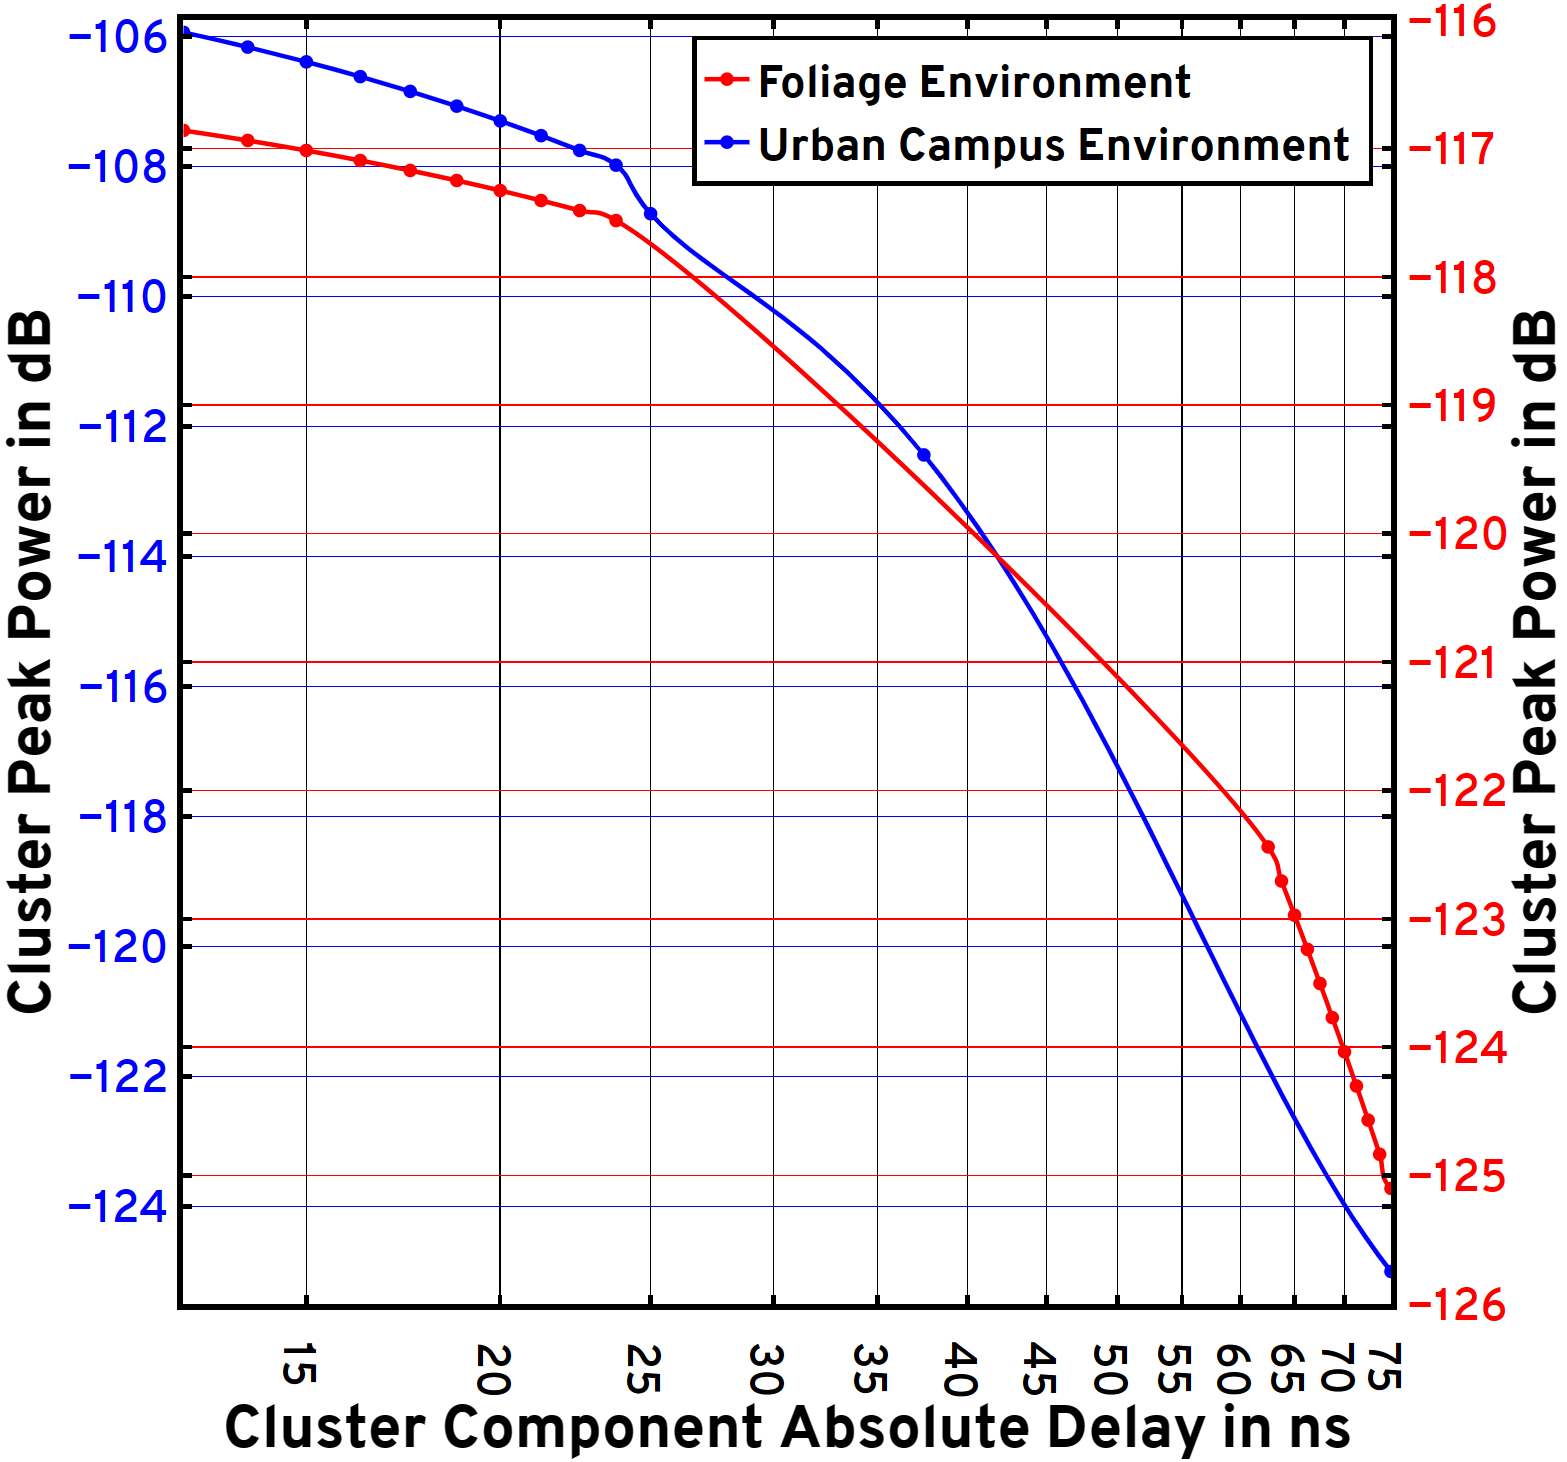
\includegraphics[width=0.97\linewidth]{figs/cluster_decay_characteristics.png}
        \caption{Cluster Decay Characteristics (\href{https://codeocean.com/capsule/9545863/tree}{CodeOcean}~\cite{CodeOcean}; \href{http://ieee-dataport.org/12580}{DataPort}~\cite{DataPort})}
        \label{F12b}
    \end{subfigure}
    \vspace{-5mm}
    \caption{The CDFs of the cluster inter-arrival times (in nanoseconds) (a) and the plot of cluster peak power (in dB) vs absolute delay (in nanoseconds) (b), for the urban campus route around $100$ S St (Rx on a push-cart), the suburban neighborhood route around S Wolcott St (Rx on a push-cart), and the foliage dominated route around the Olpin Union building (Rx on a push-cart). Fig.~\ref{F12a} also depicts the CDFs derived from the SV~\cite{SV_Molisch} and stochastic~\cite{Indoor60G} models.}
    \vspace{-6mm}
    \label{F12}
\end{figure*}
where $l$ is the MPC index ($1$ to $L$), $\phi_{l}$ is the azimuth AoA for the $l^{\mathrm{th}}$ MPC while $\theta_{l}$ is its elevation AoA, $P(\phi_{l}, \theta_{l})$ is the normalized power spectrum at $\phi_{l}$ and $\theta_{l}$, $\boldsymbol{\mu}_{\Omega}$ is the mean direction (described in~\cite{Indoor60G}), and $\mathbf{e}(\phi_{l}, \theta_{l})$ is the direction unit vector for the $l^{\mathrm{th}}$ MPC (described in~\cite{Indoor60G}). Fig.~\ref{F11b} also illustrates the direction spread CDFs derived from the SV~\cite{SV_Molisch} and stochastic~\cite{Indoor60G} mmWave channel models. Furthermore, as is the case in our RMS delay spread investigations, we evaluate the Kolmogorov-Smirnov statistic for the RMS AoA direction spread wherein we calculate the aforementioned statistical distance between the empirical CDF of the RMS AoA direction spread obtained from our measurements and the CDFs of the reference distributions outlined by the SV and stochastic mmWave channel models. Here, again, under our Kolmogorov-Smirnov statistical analysis, we note that the stochastic channel model~\cite{Indoor60G} ($0.174$) demonstrates \emph{a better fit} with our measurements around the urban campus environment, relative to the SV~\cite{SV_Molisch} ($0.634$) model. Moreover, perusing Fig.~\ref{F11b}, we can deduce that mmWave signals in our V$2$X measurements around the foliage environment experience a larger spread in the angles-of-arrival at the receiver, due to the larger number of reflections and scattering/diffraction effects induced by the thick vegetation along this route, as opposed to the urban campus and suburban neighborhood environments. Finally, Fig.~\ref{F12a} illustrates the empirical CDFs of the cluster inter-arrival times obtained from our onsite measurements at the NSF POWDER testbed, with the Rx traversing unplanned routes around the urban campus, suburban neighborhood, and foliage environments. Again, Fig.~\ref{F12a} depicts CDFs of the cluster inter-arrival times as detailed by the SV~\cite{SV_Molisch} and stochastic~\cite{Indoor60G} channel models: here, both model demonstrate similarly large statistical distances ($0.71$) leading to \emph{subpar representations} of our measurements. Lastly, Fig.~\ref{F12b} depicts the empirical cluster decay characteristics (cluster peak power as a function of its absolute delay) for V$2$X routes around the urban campus and foliage environments. Here, as expected, we observe that the cluster peak power decreases with increasing delay as a result of the higher attenuations experienced by the longer (i.e., larger delay) signal paths, resulting from reflections and scattering/diffraction effects induced by the terrain and/or obstacle profiles at the measurement site.
\vspace{-3mm}

% Concluding remarks and Future work
\section{Conclusion}\label{S6}
In this work, we discuss the design of a fully autonomous beam-steering platform coupled with a broadband sliding correlator channel sounder, best-suited for mmWave V$2$X modeling. Corroborated onsite, this beam-steering system demonstrates superior performance vis-\`{a}-vis geo-positioning accuracy, alignment reliability, and tracking response times. Processing the recorded power delay profiles via custom noise elimination and thresholding heuristics, we perform pathloss evaluations against the widely used $3$GPP TR$38.901$, ITU-R M$.2135$, METIS, and mmMAGIC outdoor urban micro- and macro-cellular standards. Herein, we demonstrate that such standards particularly fail to accurately model the pathloss vs log-distance behavior of \SI{28}{\giga\hertz} signals in V$2$X networks within urban, suburban, and foliage environments. Along with shadow fading investigations, we report (and compare against the D$2$D model) the average fade depth and duration metrics, under static (buildings) and dynamic (pedestrians, moving/parked vehicles) blockages. Crucially, the continuous series of measurements facilitated by our design enables decoherence studies under distance and alignment accuracy effects, wherein we demonstrate rapid decorrelation for minor distance and alignment changes. Lastly, centered around the Kolmogorov-Smirnov statistic, multipath clustering analyses enable the empirical validations of the SV, QD, and stochastic channel models vis-\`{a}-vis the cluster inter-arrival times, cluster decay characteristics, and RMS delay and direction spreads.
\vspace{-3mm}

% References (main.bib)
\balance
\bibliographystyle{IEEEtran}
\bibliography{IEEEabrv,main}

\end{document}
% Content ends